\documentclass[12pt,twoside,openright,a5paper]{book}
\usepackage[margin=0.75in]{geometry}
\usepackage{layout}
\usepackage{pgffor}
\usepackage{tocloft}
\usepackage[table, dvipsnames]{xcolor}
\usepackage{fontspec}
\usepackage{fancybox}
\usepackage[skins]{tcolorbox}
\usepackage{fancyhdr}
\usepackage{setspace}
\usepackage[utf8]{inputenc}
\usepackage{emptypage}
\usepackage[vskip=0pt,rightmargin=0cm]{quoting}
\usepackage{sectsty}
\usepackage{polyglossia}
\usepackage{changepage}%
\usepackage{imakeidx}
\usepackage{setspace}
\usepackage{longtable,array}
\usepackage{tikz} % Package for drawing
\usepackage{tikzpagenodes}
\usepackage[toc,acronym]{glossaries}
\usepackage{fontawesome5}
\usepackage{marvosym}
\usepackage[totoc, font=footnotesize]{idxlayout}
\usepackage{eso-pic} % background image in titlepage
\usepackage{anyfontsize} % any font size
% Remove this package for the final copy
\newfontfamily\engfont[Script=Kannada]{Arial Unicode MS}
\usepackage[hpos=24mm,fontsize=32pt, hanchor=l,anchor=lc,angle=90,color={[gray]{0.5}}, text={\engfont{DRAFT \ COPY}}]{draftwatermark}




\newfontfamily\engfont[Script=Kannada]{Noto Serif Kannada}
\usepackage[hpos=24mm,fontsize=32pt, hanchor=l,anchor=lc,angle=90,color={[gray]{0.5}}, text={\engfont{DRAFT \ COPY}}]{draftwatermark}

\newskip\linepagesep \linepagesep 5pt\relax
\renewcommand\footrulewidth{0.5pt}
\def\vfootline{%
    \begingroup
        \color{blue}\rule[-990pt]{20pt}{1000pt}
    \endgroup}



\setmainfont[Script=Kannada, Renderer=HarfBuzz, LetterSpace=12]{Noto Serif Kannada}
\setmainlanguage[numerals=kannada]{kannada}
\setotherlanguages{english}
\newfontfamily\kannadafont[Script=Kannada]{Noto Serif Kannada}
\newfontfamily\kannadafontsf[Script=Kannada]{Noto Serif Kannada}
\newfontfamily\kanBold[Script=Kannada]{Noto Serif Kannada Bold}
\newfontfamily\kanfont[Script=Kannada]{Noto Serif Kannada}
\newfontfamily\mananamfont[Script=Kannada, Scale=1]{NudiUni08k}
\newfontfamily\mananamtext[Script=Kannada, Scale=0.75]{Noto Serif Kannada}
\fancyhf{}
  \fancyfoot[RO]{\vfootline\hskip\linepagesep\thepage}
  \fancyfoot[LE]{\thepage\hskip\linepagesep\vfootline}
  \fancyhead[RO]{\small\kanfont ದಿನಾಂಕ ..../..../.....}
  \fancyhead[LO]{\small\kanfont ಗೀತಾ ಮನನಂ}
  \fancyhead[LE]{\small\kanfont ಗೀತಾ ಮನನಂ}
  \fancyhead[RE]{\small\kanfont ದಿನಾಂಕ ..../..../.....}
  \renewcommand\headrulewidth{1pt}
  \fancypagestyle{plain}{%
    \fancyhf{}
    \fancyfoot[RO]{\vfootline\hskip\linepagesep\thepage}
    \fancyfoot[LE]{\thepage\hskip\linepagesep\vfootline}
    \renewcommand\headrulewidth{0pt}
  }
\quotingsetup{font={itshape,footnotesize}}
\title{\Huge \kanfont \textbf{ಗೀತಾ ಮನನಂ}\\
{\normalsize Gita Mananam\\}
{\small(ದೈನಂದಿನ ಸ್ಪೂರ್ತಿ ಹಾಗೂ ಆತ್ಮಾವಲೋಕನಕ್ಕಾಗಿ)}}
\author{\large \kanfont ಸ್ವಾಮಿ ನಿರ್ಗುಣಾನಂದಗಿರಿ\\
{\normalsize Swamy Nirgunanandagiri}\\
\vspace{15mm}
{\normalsize Bhageeratha Publications}\\
{Rishikesh, India}
}


\addto\captionskannada{\renewcommand{\contentsname}{\color{blue}{ವಿಷಯ ಸೂಚಿ}}} 

% Reduce space between TOC
\setlength\cftparskip{-2pt}
\setlength\cftbeforechapskip{2pt}
\setcounter{secnumdepth}{-1}
\chapterfont{\color{blue}}  % sets colour of chapters
\setlength\parindent{0pt} % no-indent for entire file
\date{} % clear date
\makeindex
\indexsetup{othercode=\small}
%%Term definitions
\mananatext{
\begin{description}
   \item[ಧರ್ಮ] ಧರ್ಮವೆಂಬುವುದು ಸಾಮಾನ್ಯತಃ, ಒಬ್ಬ ವ್ಯಕ್ತಿಯ ಜೀವನದಲ್ಲಿ, ಸಮಾಜದಲ್ಲಿ ಹಾಗೂ ಪ್ರಕೃತಿಯ ನಿಯಮಕ್ಕೆ ಹೊಂದಿಕೊಂಡು ಹೋಗುವಂತಹ, ಅವನ ನೈತಿಕ ಬಾಧ್ಯತೆ ಕರ್ತವ್ಯಗಳ ಮಹತ್ವವನ್ನು ಸೂಚಿಸುತ್ತದೆ. ಗೀತೆ ಮತ್ತು ವೇದಗಳ ದೃಷ್ಟಿಕೋನದಿಂದ ನೋಡಿದರೆ, ಕೇವಲ ಲೌಕಿಕ ಲಾಭಗಳಿಗೆ ಮಾತ್ರವಲ್ಲದೇ, ಆಧ್ಯಾತ್ಮಿಕ ಜೀವನ ಮತ್ತು ಮೋಕ್ಷದ ಅನ್ವೇಷಣೆಗಾಗಿ ಧರ್ಮದ ಪರಿಪಾಲನೆ ಮಾಡುವುದೇ ಆಗಿದೆ. ಅಹಂ ಮತ್ತು ಅದರ ಇಷ್ಟಾನಿಷ್ಟಗಳನ್ನು ಮೆಟ್ಟಿ, ಈ ಸೃಷ್ಟಿಯ ದೈವೀಕ ಯೋಜನೆಗೆ ಅನುಗುಣವಾಗಿ ಜೀವಿಸುವುದೇ ಧರ್ಮದ ಕರೆಯಾಗಿದೆ.
   \item[ಭಗವಂತ] ಭಗವಾನ್ ಎಂದರೆ, ಆರು ದೈವೀಕ ಗುಣಗಳಾದ  ಪ್ರಭುತ್ವ, ಅಧಿಕಾರತ್ವ, ಖ್ಯಾತಿ, ಶಕ್ತಿ, ಜ್ಞಾನ ಮತ್ತು ತಟಸ್ಥತೆ ಹೊಂದಿರುವ ಒಂದು  ಪದವಿ. ಗೀತೆಯಲ್ಲಿ ಭಗವಾನ್ ಎಂದರೆ,  ‘ಪರಮಗುರು’;  ಸಾಕಾರ ರೂಪದಲ್ಲಿರುವ ಆ ಪರಮಾತ್ಮನೇ; ಗ್ರಹಣಾಕಾಂಕ್ಷಿಯಾದ ಸಾಧಕನಿಗೆ ಕರುಣೆಯಿಂದ ಮುಕ್ತಿಮಾರ್ಗಕ್ಕೆ ಬೇಕಾದ ವಿವೇಕವನ್ನು ದಯಪಾಲಿಸುವವನು ; ಶ್ರದ್ಧಾಳು ಭಕ್ತರಿಗೆ ಭಗವಂತನೆಂದರೆ ಪರಮ ಆಶ್ರಯದಾತನು ಹಾಗೂ, ಆತ್ಮಸಾಕ್ಷಾತ್ಕಾರಕ್ಕಾಗಿ ಮಾರ್ಗವನ್ನು ತೋರಿಸುವ ದೀವಿಗೆ.
   \item[ಸ್ಥಿತಪ್ರಜ್ಞ] ಯಾವ ವ್ಯಕ್ತಿಗೆ ಸ್ಥಿರವಾದ ವಿವೇಕ ಮತ್ತು ಬುದ್ಧಿಶಕ್ತಿ ಇರುವುದೋ, ಯಾರು ಸದಾ ಸಮಚಿತ್ತತೆಯಿಂದ ಇರುವನೋ, ಯಾರ ಇಂದ್ರಿಯಗಳು ಅವನ ಹಿಡಿತದಲ್ಲಿರುವುವೋ, ಯಾರು ಆಸೆ ಮತ್ತು ಭಯದಿಂದ ಮುಕ್ತನೋ ಹಾಗೂ, ಜೀವನದಲ್ಲಿ ಸಂತೋಷ ಬಂದಾಗ ತೀರಾ ಹಿಗ್ಗದೇ, ದುಃಖ ಬಂದಾಗ ಹತಾಶನಾಗದೇ ಇರುವನೋ,ಅಂಥವನು ‘ಸ್ಥಿತಪ್ರಜ್ಞ’ ; ಅಲ್ಲದೇ, ಯಾವನು ತನ್ನ ಆತ್ಮದಲ್ಲಿಯೇ ಸಂತೃಪ್ತನೋ, ಹಾಗೂ ಸಾಮಾನ್ಯತಃ, ಆತ್ಮಜ್ಞಾನವಿಲ್ಲದ ಒಬ್ಬನಿಗೆ ಕಾಡುವ ಅಪೂರ್ಣತೆಯ ಭಾವನೆ ಯಾವನಿಗೆ ಇಲ್ಲವೋ, ಅವನೇ ‘ಸ್ಥಿತಪ್ರಜ್ಞ’ ಎಂದೆನಿಸಿಕೊಳ್ಳುತ್ತಾನೆ.
\end{description}
}
%\makeglossaries


\newcommand\Linepage[1][0.40in]{% Change to suit
  \vbox to \dimexpr\textheight-\pagetotal-#1\relax {% Let TeX do the work...
    \leaders\hbox to \linewidth{\rule{0pt}{#1}\hrulefill}\vfil
  }%
}

\newtcolorbox{inspiration}[2][]{%
  floatplacement=b,float, 
  enhanced,colback=white,colframe=purple,coltitle=black,
  sharp corners,boxrule=1pt, width=\textwidth,
  fonttitle=\sffamily\scshape\color{teal},
  rightrule=3mm,
  fontupper=\itshape,
  fontlower=\tiny,
  attach boxed title to top left={yshift=-0.5\baselineskip-0.4pt,xshift=2mm},
  boxed title style={tile,size=minimal,left=0.5mm,right=0.5mm,
    colback=white,before upper=\strut},
  title=#2,#1
}
\newtcolorbox{mananam}[2][fontlower=\small]{%
  enhanced,colback=white,colframe=teal,coltitle=black,
  sharp corners,boxrule=1pt, width=\textwidth,
  fonttitle=\sffamily\scshape\color{purple},
  leftrule=3mm,
  fontupper=\itshape,
  fontlower=\tiny,
  attach boxed title to top left={yshift=-0.5\baselineskip-0.4pt,xshift=4mm},
  boxed title style={tile,size=minimal,left=0.5mm,right=0.5mm,
    colback=white,before upper=\strut},
  title=#2,#1
}



% commands
\definecolor{aurometalsaurus}{rgb}{0.43, 0.5, 0.5}
\newcommand{\slcol}[1]{{\color{MidnightBlue}{#1}}}
\newcommand{\cquote}[1]{\begin{quoting}{\color{black}{#1}}\end{quoting}}
%% Custom macro to convert Arabic numerals to Kannada numerals
\makeatletter
\newcommand{\converttoKannada}[1]{%
  \ifcase#1 ೦\or ೧\or ೨\or ೩\or ೪\or ೫\or ೬\or ೭\or ೮\or ೯\else\expandafter\converttoKannadaLoop\fi
}
\newcommand{\converttoKannadaLoop}[1]{%
  \expandafter\converttoKannada\expandafter{\the\numexpr#1/10}\converttoKannada{\the\numexpr#1\mod10}%
}
\makeatother

% Redefine page numbering globally to use Kannada numerals
\renewcommand{\thepage}{\converttoKannada{\arabic{page}}}

% Redefine index page numbers (the page numbers shown in the index itself)
\renewcommand{\index}{\@ifnextchar[{\@indexwithpage}{\@indexwithoutpage}}

\def\@indexwithpage[#1]#2{\indexentry{#2}{\converttoKannada{#1}}}
\def\@indexwithoutpage#1{\indexentry{#1}{\converttoKannada{\thepage}}}
\renewcommand{\cftchapfont}{\normalfont}
\renewcommand{\cftchappagefont}{\normalfont}
%column decoration
\setlength{\columnseprule}{1pt}
\def\columnseprulecolor{\color{blue}}

\begin{document}

\pagenumbering{roman}
\begin{titlepage}
	%\pagecolor{pastelblue}
	\AddToShipoutPictureBG*{%
    \AtPageLowerLeft{%
        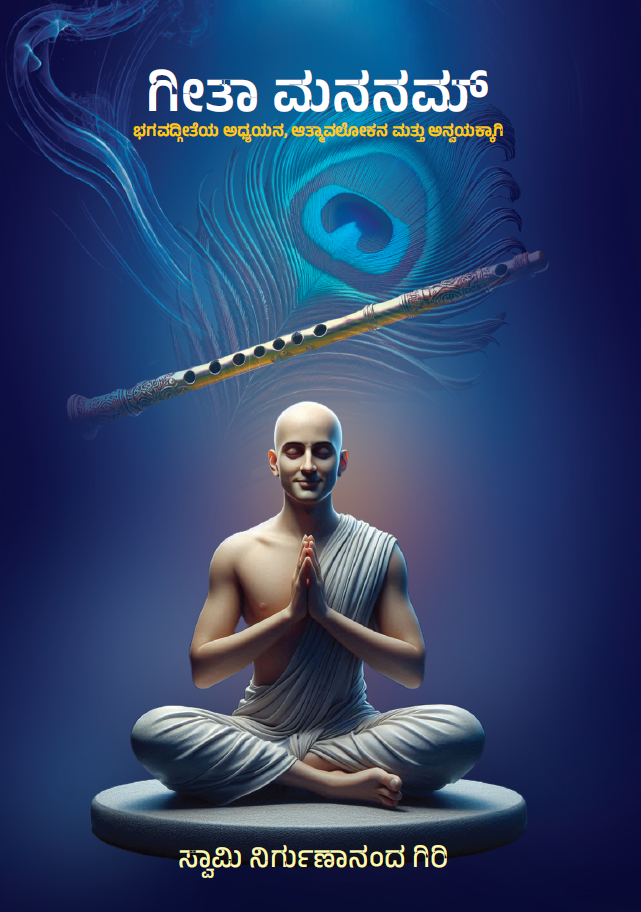
\includegraphics[width=\paperwidth,height=\paperheight]{./images/frontcover.png}%
    }%
}
    \begin{center}
        \vspace*{0.5cm}
            
        {\Huge
        %\textbf{\color{white}\fontsize{50}{60}\selectfont ಗೀತಾ ಮನನಂ}
		}
        %\textbf{\\ \small \color{white}ದೈನಂದಿನ ಸ್ಪೂರ್ತಿ ಹಾಗೂ ಆತ್ಮಾವಲೋಕನಕ್ಕಾಗಿ}    
        \vspace{1.0cm}
            
        
		
            
        \vfill
            
        
            
        \vspace{0.1cm}
        {\color{white}    
		%\textbf{{\Large \mananamfont ಸ್ವಾಮಿ ನಿರ್ಗುಣಾನಂದ ಗಿರಿ}}\\
		%{\normalsize Swami Nirgunananda Giri\\Rishikesh, India}
		}
    \end{center}
\end{titlepage}
\nopagecolor% Use this to restore the color pages to white
\begin{titlepage}
	%\pagecolor{pastelblue}
	%\AddToShipoutPictureBG*{%
    %\AtPageLowerLeft{%
    %    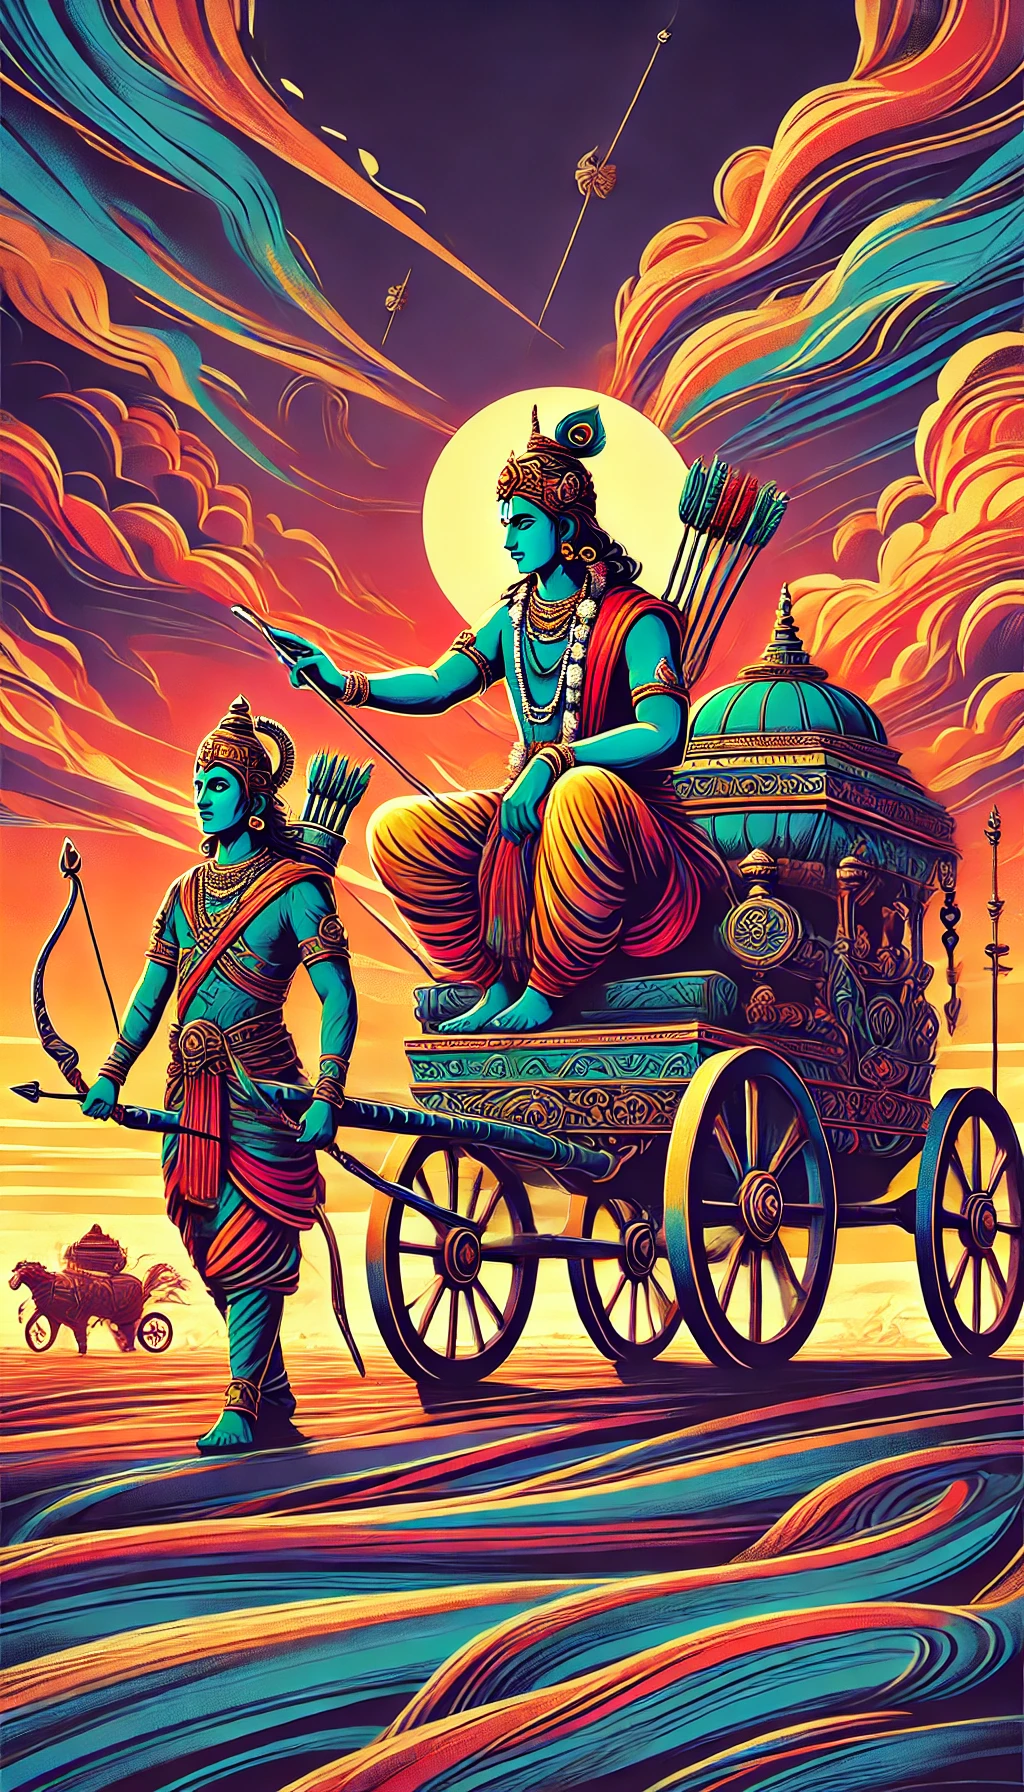
\includegraphics[width=\paperwidth,height=\paperheight]{./images/krishna4.jpg}%
    %}%
%}
    \begin{center}
        \vspace*{0.5cm}
            
        {\Huge
        \textbf{\color{blue}\fontsize{50}{60}\selectfont ಗೀತಾ ಮನನಂ}}
        \textbf{\\ \small \color{black}ದೈನಂದಿನ ಸ್ಪೂರ್ತಿ ಹಾಗೂ ಆತ್ಮಾವಲೋಕನಕ್ಕಾಗಿ}\\    
        \vspace{1.0cm}
		    \textbf{{\large \color{black} ಅಧ್ಯಾಯ ೫ ಕರ್ಮ ಸನ್ಯಾಸ ಯೋಗ}}\\		
        \vspace{6.0cm}
        \textbf{{\Large \color{blue}\mananamfont ಸ್ವಾಮಿ ನಿರ್ಗುಣಾನಂದ ಗಿರಿ}}\\    
        
		
            
        \vfill
            
        
            
        \vspace{0.1cm}
        {\color{black}    
		
		{{\large \color{blue}ಹೃಷೀಕೇಶ, ಉತ್ತರಾ ಖಂಡ}\\\normalsize ಭಾರತ}
        }
    \end{center}
\end{titlepage}
\nopagecolor% Use this to restore the color pages to white
%\maketitle

\thispagestyle{empty}
Copyright \textcopyright\ Swamy Nirgunanandagiri\\
\\
All rights reserved\\
\\
Edition - First, 2024\\
\vfill
Without written permission of the author it is forbidden to reproduce or adapt in any form or by any means any part of this  publication.\\
\\
Rishikesh, India\\
\newpage
\thispagestyle{empty}
\frontmatter

\doublespacing
\tableofcontents
\singlespacing
%\clearpage
%\newgeometry{margin=0pt} % Apply margin only for this page
%\thispagestyle{empty}
%\begin{center}
%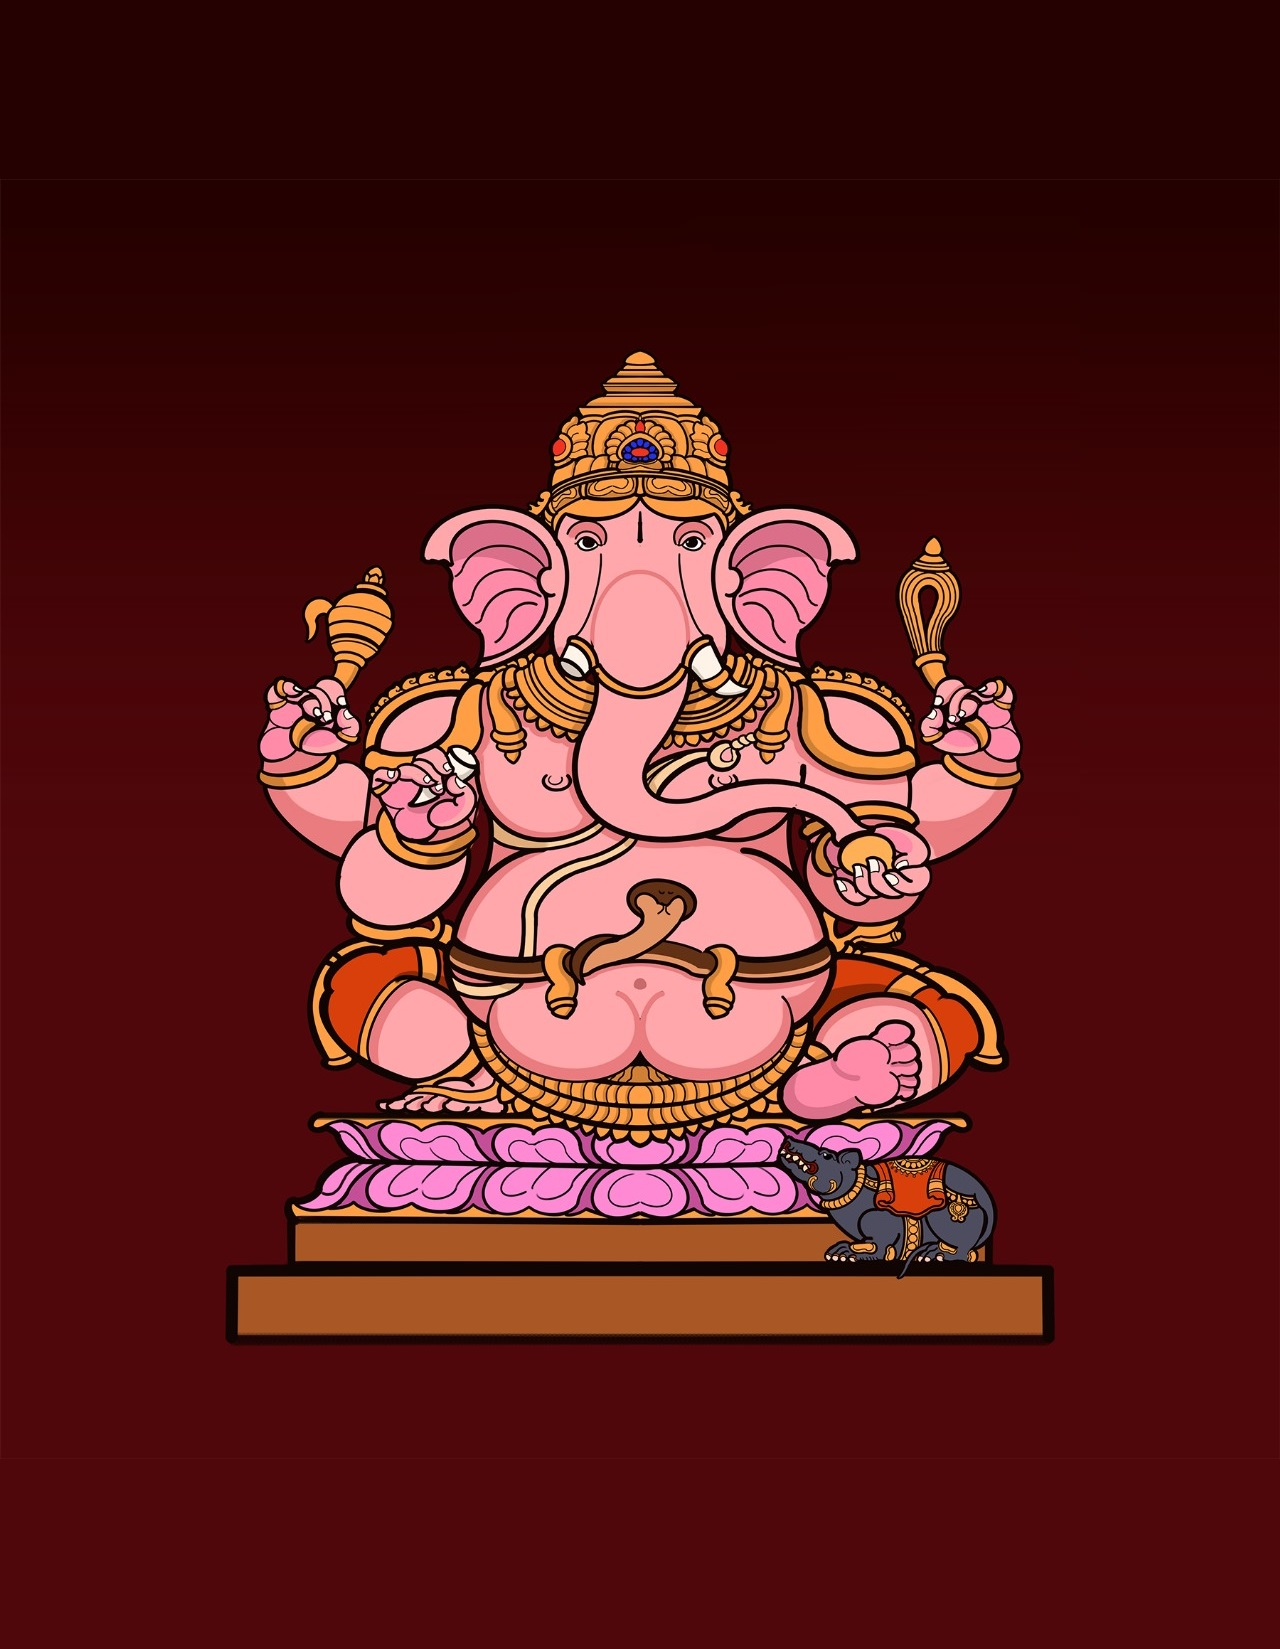
\includegraphics[width=0.9\textwidth, height=\paperheight, keepaspectratio]{./images/ganapa.jpg}
%\end{center}
%\restoregeometry % Restore original geometry settings
%\newpage

\clearpage
\newgeometry{margin=0pt} % Apply margin only for this page
\thispagestyle{empty}
%\begin{figure}
%\centering
%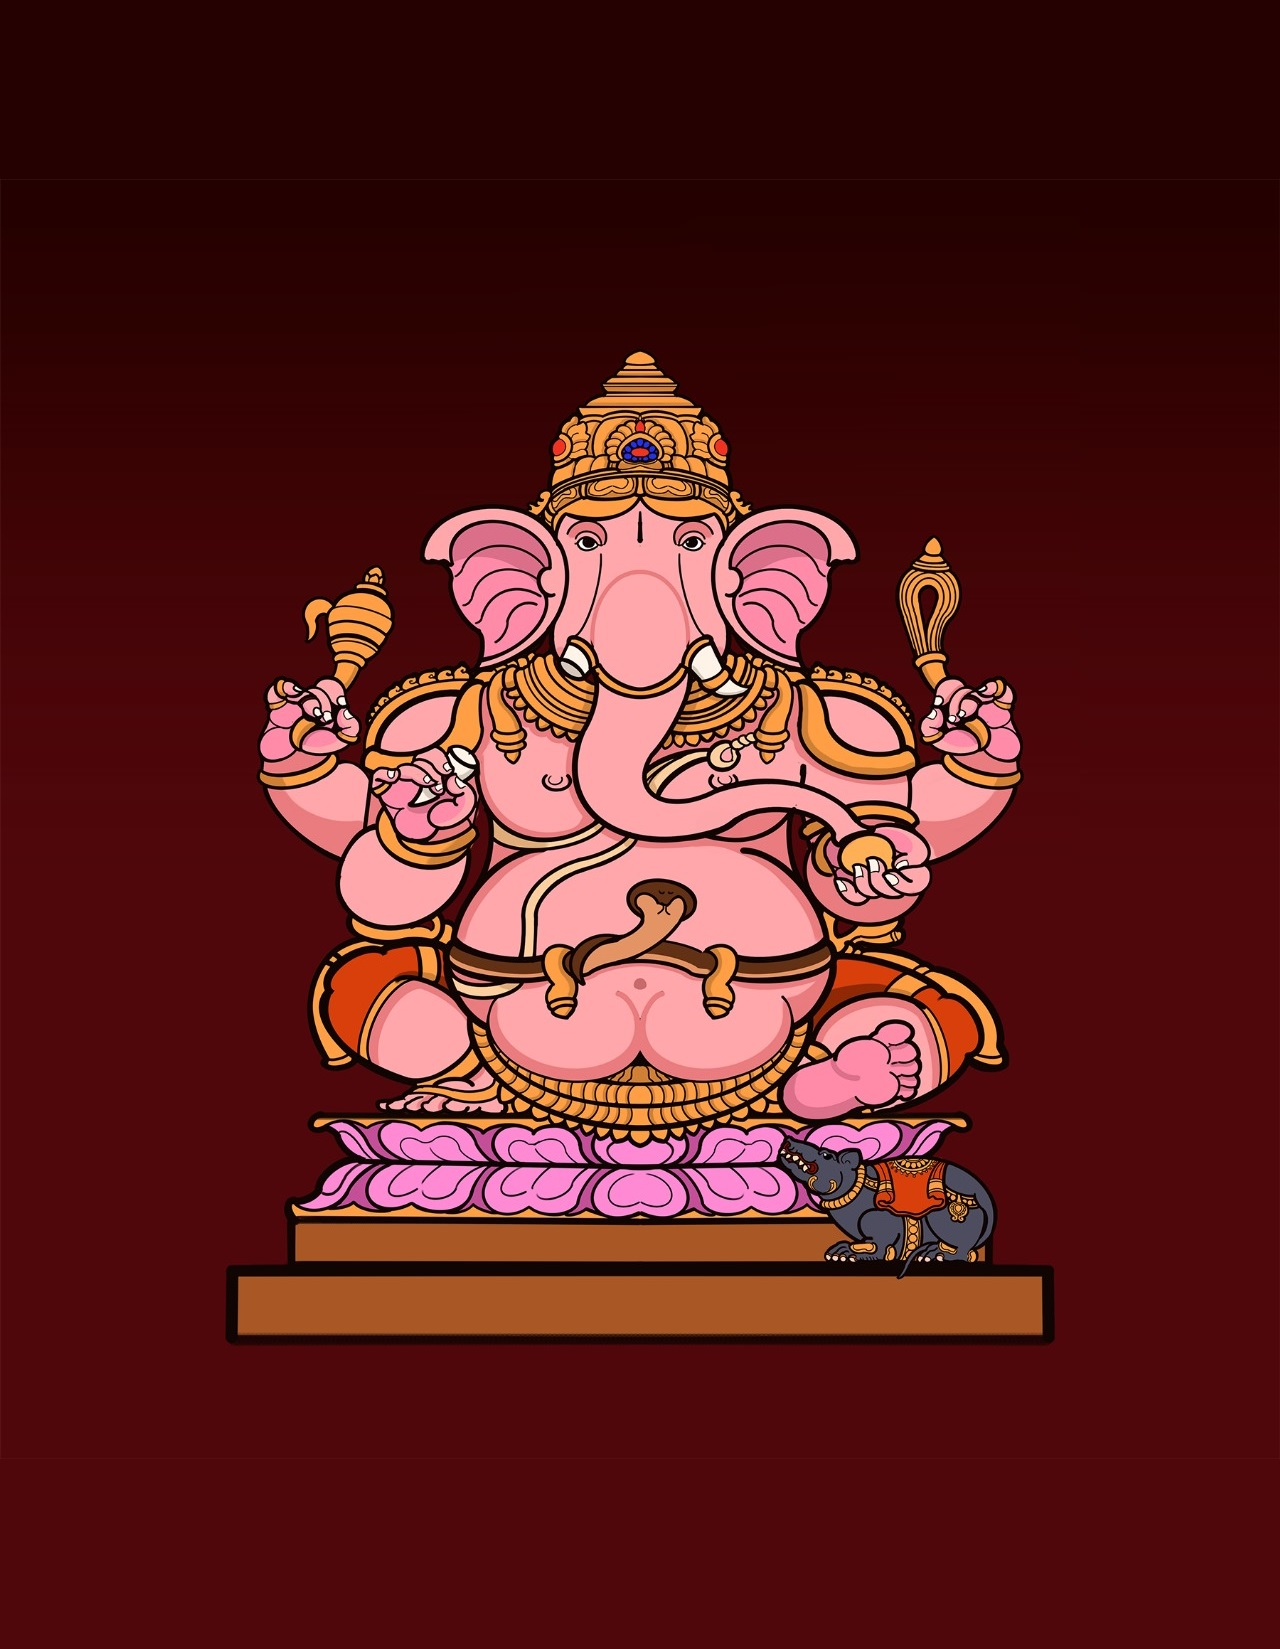
\includegraphics[width=0.9\textwidth, height=\paperheight, keepaspectratio]{./images/ganapa.jpg}
%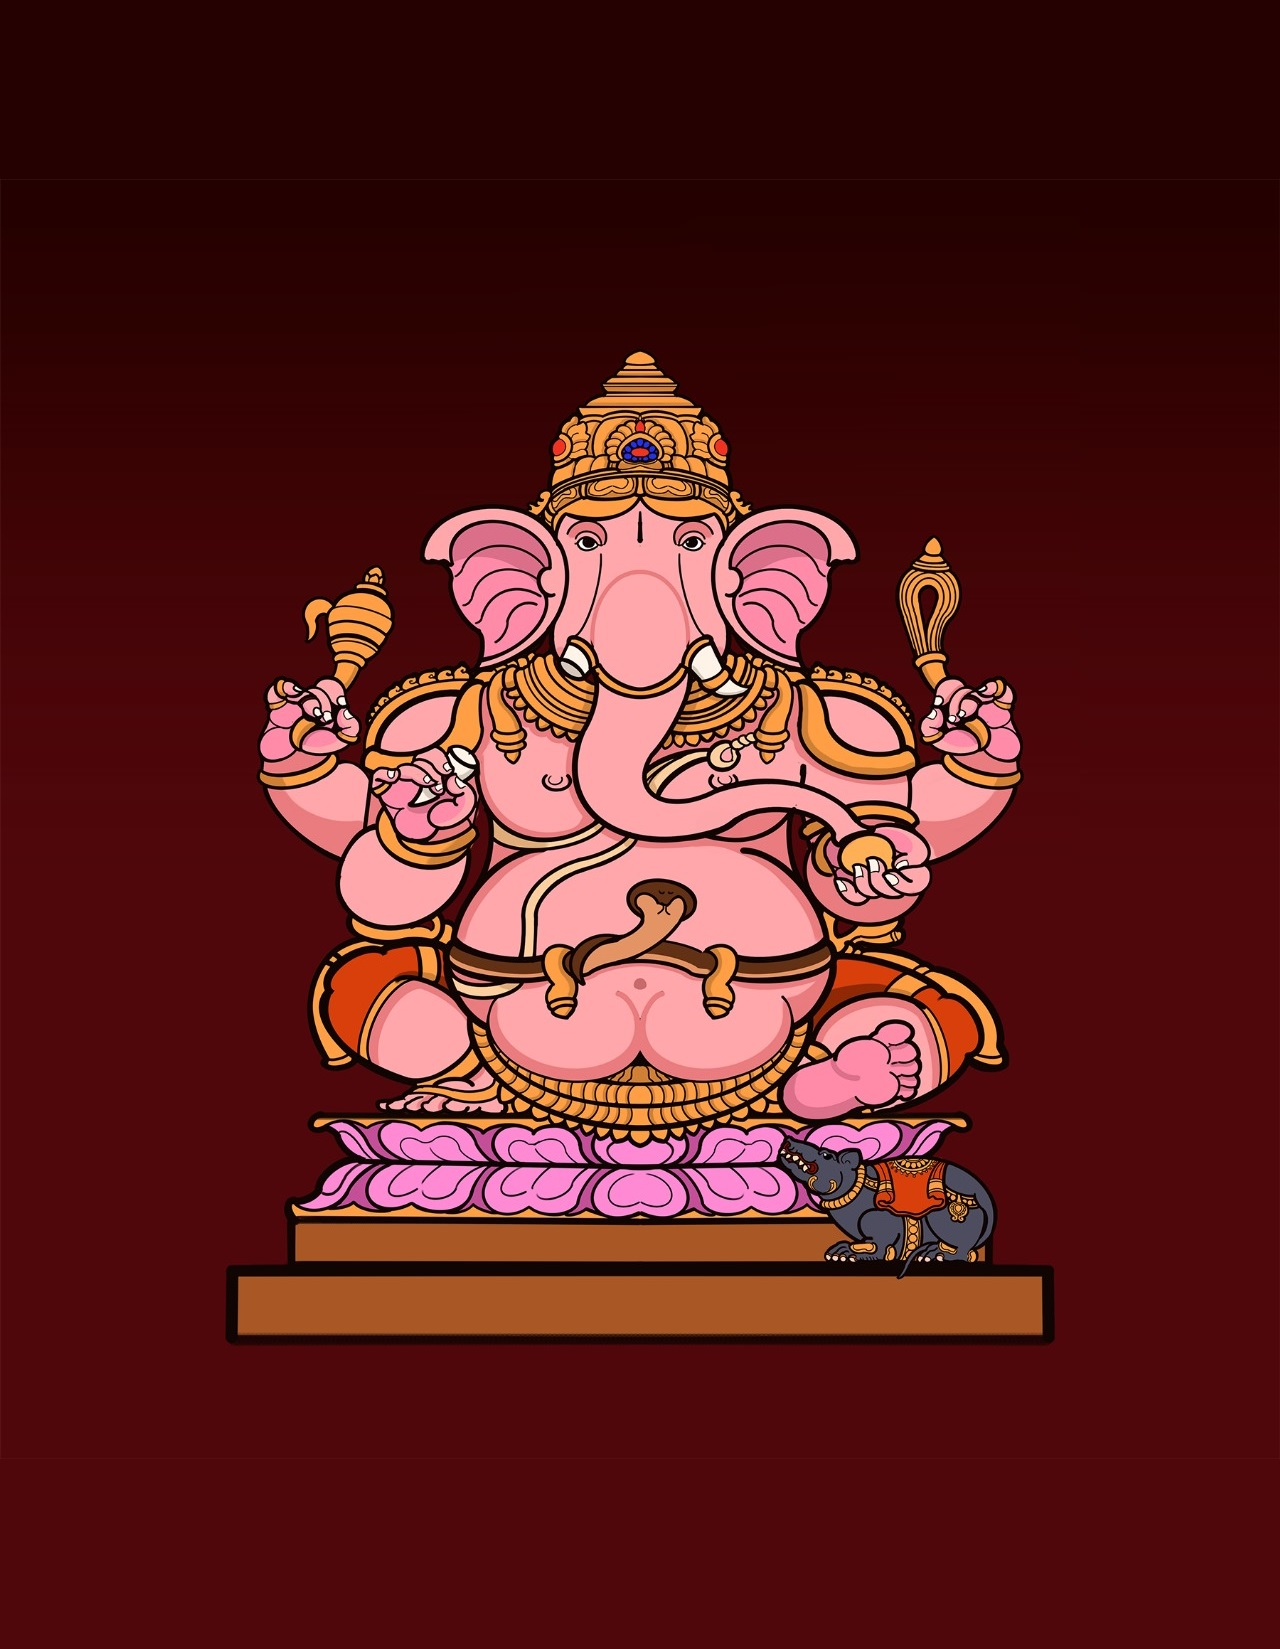
\includegraphics[width=\paperwidth, height=\paperheight]{./images/ganapa.jpg}
%\end{figure}
%\restoregeometry % Restore original geometry settings
%\newpage

\begin{figure}[h!]
    \centering
    \begin{overpic}[width=\paperwidth, height=\paperheight]{../images/001.jpg}
        \put(13,85){\color{white}\kanfont ಗಜಾನನಂ ಭೂತಗಣಾದಿ ಸೇವಿತಂ ಕಪಿತ್ಥ ಜಂಬೂಫಲಸಾರ ಭಕ್ಷಿತಮ್। }\put(10,82){\color{white}\kanfont ಉಮಾಸುತಂ ಶೋಕ ವಿನಾಶಕಾರಣಂ ನಮಾಮಿ ವಿಘ್ನೇಶ್ವರ ಪಾದಪಂಕಜಮ್॥ }
    \end{overpic}
    \caption{This is the standard figure caption below the image.}
    \label{fig:example}
\end{figure}

\restoregeometry

\thispagestyle{empty}
\thispagestyle{empty}
\pagestyle{fancy}


\chapter{\kanfont ಮುನ್ನುಡಿ}
\begin{center}
ದಿಶಂತು ಶಂ ಮೇ ಗುರುಪಾದಪಾಂಸವಃ ॥\\
\end{center}
\footnotesize \mananamtext{ಶ್ರಿ\!\char"0CD5ಮದ್ ಭಗವದ್ಗೀತೆಯು ಎಲ್ಲಾ ಧರ್ಮಗ್ರಂಥಗಳಲ್ಲಿ ಒಂದು ಅನನ್ಯ ಮತ್ತು ಸಾಟಿಯಿಲ್ಲದ ರತ್ನವಾಗಿದೆ.  ಇದು ಪರಿತ್ಯಾಗ ಮಾಡುವವರಿಗೆ ಮಾತ್ರವಲ್ಲದೆ ಲೌಕಿಕ ಜವಾಬ್ದಾರಿಗಳನ್ನು ಹೊತ್ತಿರುವವರಿಗೂ ಮಾರ್ಗದರ್ಶಿ ಬೆಳಕಾಗಿ ಕಾರ್ಯನಿರ್ವಹಿಸುತ್ತದೆ, ಆಧ್ಯಾತ್ಮಿಕದೊಂದಿಗೆ ಪ್ರಾಪಂಚಿಕತೆಯನ್ನು ಸಮತೋಲನಗೊಳಿಸಲು ಪ್ರಯತ್ನಿಸುತ್ತದೆ; ಇದು, ಅಜ್ಞಾನದಿಂದ ಅವರು (ಸಾಮಾನ್ಯ ಜನ) ತಮ್ಮನ್ನು ತಾವು,   ದೇಹ ಮತ್ತು ಮನಸ್ಸಿನ ವ್ಯವಹಾರಗಳ  ಜೊತೆ ಗುರುತಿಸಿಕೊಂಡಾಗ, ಅಂತಹ ವ್ಯವಹಾರಗಳ ಬಗ್ಗೆ ನಿಷ್ಪಕ್ಷಪಾತವಾಗಿರುವಂತೆ ಪ್ರತಿಪಾದಿಸುತ್ತದೆ.\\
ಜೀವನದಲ್ಲಿ ಒಬ್ಬರ ಕರ್ತವ್ಯಗಳನ್ನು ಸಾಧಿಸಲು, ಬಾಂಧವ್ಯದ ಅಥವಾ, ಮೋಹದ ಭಾವನೆ ಇರಬೇಕು ಎಂಬುದು ಒಂದು ತಪ್ಪು ಕಲ್ಪನೆ.  ಭಗವಾನ್ ಕೃಷ್ಣ, ಎಲ್ಲರಿಗಿಂತಲೂ  ದೊಡ್ಡ ಸಂಸಾರಿ ಹಾಗೂ, ಪರಿಪೂರ್ಣವಾದ ಮೋಹರಹಿತನಾದ ಅಸಂಸಾರಿ; ದಿವ್ಯವಾದ ಆನಂದದಲ್ಲಿ ನೆಲೆಗೊಂಡು, ಈ ಮೂರ್ತ, ಭೌತಿಕ ಜಗತ್ತಿನಲ್ಲಿ ಹೇಗೆ ಕಾರ್ಯನಿರ್ವಹಿಸಬೇಕು ಎಂಬುದನ್ನು ಅವನು ತನ್ನ ಕಾರ್ಯಗಳು, ಭಾವ ಮತ್ತು ಅವನು ಉಚ್ಛರಿಸುವ ಪ್ರತಿಯೊಂದೂ ಪರಮಪದದ  ಮೂಲಕ ಪ್ರದರ್ಶಿಸುತ್ತಾನೆ. ಆರಂಭದಲ್ಲಿ ‘ಸಂಘರ್ಷ ಮತ್ತು ಸವಾಲುಗಳಿಂದ ತುಂಬಿರುವ ಮಾರ್ಗ’ ಎಂದು ಕಂಡುಬoದರೂ ಸಹ, ಈ ಸ್ಥಿತಿಯನ್ನು ಸಾಧಿಸಲು (ದಿವ್ಯವಾದ ಆನಂದದಲ್ಲಿ ನೆಲೆಗೊಂಡು, ಈ ಮೂರ್ತ, ಭೌತಿಕ ಜಗತ್ತಿನಲ್ಲಿ  ಕಾರ್ಯನಿರ್ವಹಿಸುವುದು) ಸಮರ್ಥ ಶಿಕ್ಷಕರಿಂದ ಸರಿಯಾದ ಮಾರ್ಗದರ್ಶನದ ಅಗತ್ಯವಿದೆ. \\
ಈ ‘ನಿಪುಣ ಮಾರ್ಗದರ್ಶಿ ಕೈಪಿಡಿ’ಯಲ್ಲಿ, ಲೇಖಕರ ಆಳವಾದ ಒಳನೋಟದಿಂದ ಅಧ್ಯಾಯ 2 ರ 52-53 ಪದ್ಯಗಳಲ್ಲಿ ಸೂಚಿಸಿದಂತೆ: “ಶಿಕ್ಷಕರ ಮತ್ತು ಧರ್ಮಗ್ರಂಥಗಳ ಉದ್ದೇಶವು ನಮ್ಮನ್ನು ಭ್ರಮೆಯಿಂದ ಜಗ್ಗಿಸಿ, ಮುಕ್ತರನ್ನಾಗಿ ಮಾಡುವುದೇ ಆಗಿದೆ. ನಾವು ನಮ್ಮ ಲೌಕಿಕ ಚಿಂತನೆಯ ಮಾದರಿಗಳನ್ನು ಬಿಟ್ಟು, ಒಂದು ಉನ್ನತ ಸತ್ಯದಲ್ಲಿ (ಪಾರಮಾರ್ಥಿಕದಲ್ಲಿ) ಆಶ್ರಯ ಪಡೆಯಲು ಪ್ರಾರಂಭಿಸುತ್ತಿದ್ದಂತೆಯೇ, ಆಧ್ಯಾತ್ಮಿಕ ಪ್ರಯಾಣದ ಒಂದು ಭಾಗವಾದ ಗೊಂದಲಗಳು ಮತ್ತು ಸವಾಲುಗಳು ಏಳುತ್ತವೆ; ಆದರೆ, ನಾವು ಹೀಗೆ ಈ ಹಾದಿಯಲ್ಲಿ ಪ್ರಗತಿ ಹೊಂದುತ್ತಿದ್ದಂತೆ, ಸ್ಪಷ್ಟತೆ ಪಡೆಯಲು ಪ್ರಾರಂಭಿಸುತ್ತೇವೆ”.\\
ಈ ಪುಸ್ತಕವು ಲೇಖಕರ ಕ್ರಾಂತಿಕಾರಿ ಚಿಂತನೆಗಳ ಮೂಲಕ ಓದುಗರನ್ನು ದೇಹದಿಂದ, ಮನಸ್ಸಿಗೆ ಮತ್ತು ಮನಸ್ಸಿನಿಂದ ಪ್ರಜ್ಞೆಗೆ (ಚೈತನ್ಯಕ್ಕೆ), ಒಬ್ಬರ ಅಸ್ತಿತ್ವದ ಪದರಗಳನ್ನು ಭೇದಿಸುವಂತೆ ಮಾಡುತ್ತದೆ. \\
ಪ್ರತಿ ವಿಭಾಗದಲ್ಲಿ, ‘ಮನನಂ’ ಶೀರ್ಷಿಕೆಯಡಿಯಲ್ಲಿರುವ ಆತ್ಮಾವಲೋಕನದ ಪ್ರಶ್ನೆಗಳು, ಸ್ವಯಂ ಸಮಾಧಾನ ಮತ್ತು ಆತ್ಮವಂಚನೆಯಲ್ಲಿ (ಆತ್ಮ ಪ್ರವಂಚನ) ತೊಡಗಿರುವವರಿಗೆ ಯಾವುದೇ ವಿರಾಮ ನೀಡುವುದಿಲ್ಲ ಮತ್ತು ಪ್ರಾಮಾಣಿಕವಾದ ಸ್ವಯಂ ಮೌಲ್ಯಮಾಪನ ಮಾಡಲು ಅವರಿಗೆ ಸವಾಲು ಒಡ್ಡುತ್ತವೆ .  ಮತ್ತೊಂದೆಡೆ, ‘ಸ್ಫೂರ್ತಿ’ಯ ಅಡಿಯಲ್ಲಿರುವ ಪದಗಳು, ಪ್ರಯಾಸಕರ ಮತ್ತು ಗೊಂದಲಮಯ ಆಧ್ಯಾತ್ಮಿಕ ಮಾರ್ಗವನ್ನು ತುಲನಾತ್ಮಕವಾಗಿ ಸುಲಭಗೊಳಿಸಿ, ಸಕಾರಾತ್ಮಕತೆಯ ಒಂದು, ಅಕ್ಷಯವಾದ ಮೂಲವಾಗಿ ಕಾರ್ಯನಿರ್ವಹಿಸುತ್ತವೆ.\\
ಈ ಕೈಪಿಡಿಯು, ಆಕಾಂಕ್ಷಿಗಳಿಗೆ ಜೀವನದ ವಿವಿಧ ಸಮಸ್ಯೆಗಳಿಗೆ ಪರಿಹಾರವನ್ನು ಕಂಡುಕೊಳ್ಳಲು ಸಾಕಷ್ಟು ಸಮಾಧಾನಗಳನ್ನು  ನೀಡುತ್ತದೆ, ಆದರೆ ಬಾಹ್ಯವಾಗಿ ಅಲ್ಲ, ಆಂತರಿಕವಾಗಿ.\\
ಈ ಪುಸ್ತಕದ ವಿಷಯವು, ‘ಮಾನವ ಮನೋವಿಜ್ಞಾನ’ದ ಬಗ್ಗೆ ಲೇಖಕರ ಆಳವಾದ ತಿಳುವಳಿಕೆಯನ್ನು ತೋರಿಸುತ್ತದೆ, ಮೊದಲು ಸಕಾರಾತ್ಮಕ ಮಾನಸಿಕ ಸ್ಥಿತಿಯ ಕಡೆಗೆ ಮತ್ತು ನಂತರ ಅದನ್ನು ಮೀರಿ, ಆಂತರಿಕ ಶಾಶ್ವತವಾದ ಆತ್ಮದೆಡೆಗೆ, ಸರಳವಾಗಿ ಮುಂದುವರಿಯುತ್ತದೆ. \\
ಈ ಪುಸ್ತಕದ ಓದುಗರು ಈ ಪ್ರಯಾಣವನ್ನು ಪ್ರಾರಂಭಿಸಿದಾಗ, ಅವರು ಖಂಡಿತವಾಗಿಯೂ ಮಾನವ ಮನಸ್ಸಿನ ಕ್ಷೇತ್ರವನ್ನು ಮೀರುತ್ತಾರೆ ಮತ್ತು ಈ ಸ್ವರ್ಗೀಯ ಗೀತೆಯಾದ  ‘ಭಗವದ್ಗೀತೆ’ ಗಾಯಕನ ಕೃಪೆಯಿಂದ ‘ಅಧಿಷ್ಠಾನ ಚೈತನ್ಯಮ್’ (ಚೇತನಾತ್ಮಕದ ಅಂತಿಮ ಮೂಲತತ್ವ) ಅನ್ನು ತಲುಪುತ್ತಾರೆ. ಸಾಧಕರ ಅನುಕೂಲಕ್ಕಾಗಿ ತಮ್ಮ ಅಮೂಲ್ಯವಾದ ಆಲೋಚನೆಗಳನ್ನು ಲೇಖಿಸಿದ, ಸ್ವಾಮಿ ನಿರ್ಗುಣಾನಂದ ಗಿರಿ, ಇವರ ನಿಸ್ವಾರ್ಥ ಪ್ರಯತ್ನವನ್ನು,  ಸನಾತನ ಗುರುವಾದ, ಆ ಭಗವಂತ ಶ್ರೀಕೃಷ್ಣನು ಆಶೀರ್ವದಿಸಲಿ.\\\\
\begin{center}
ಮಂಗಳಂ ಸರ್ವಂ
\end{center}

{\kanBold ಸ್ವಾಮಿ ಸ್ವಾನಂದ ತೀರ್ಥ} \\
ಆಚಾರ್ಯ, ಕೈಲಾಸ್ ಆಶ್ರಮ\\
ಋಷಿಕೇಶ – ಉತ್ತರಖಂಡ\\
}
%\thispagestyle{empty}
\begin{onehalfspace}
\chapter{\kanfont ಪ್ರಸ್ತಾವನೆ}
\footnotesize \mananamtext{ನಾವೆಲ್ಲರೂ ಜೀವನದ ಹೋರಾಟಗಳನ್ನು ಎದುರಿಸಲೇಬೇಕು. ಕುರುಕ್ಷೇತ್ರ ಯುದ್ಧದಲ್ಲಿ ಶ್ರೀ ಕೃಷ್ಣ ಪರಮಾತ್ಮನು, ತನ್ನ ವೇದನಾಯುಕ್ತ ಶಿಷ್ಯ ಅರ್ಜುನನಿಗೆ, ಪ್ರಾಪಂಚಿಕತೆಯಲ್ಲಿಯೂ ಅಧ್ಯಾತ್ಮಿಕತೆಯನ್ನು ಆಚರಣೆಗೆ ತರುವಂತಹ, ಸಂಕ್ಷಿಪ್ತ ಹಾಗೂ ಪ್ರಾಯೋಗಿಕವಾದ,  ಅತೀ ಪವಿತ್ರವಾದ ಬೋಧನೆಗಳನ್ನು ಕೊಟ್ಟಿದ್ದಾನೆ. ಈ ಶ್ರೇಷ್ಠವಾದ ಉಪನಿಷತ್ತುಗಳ ಸತ್ವಗಳನ್ನೊಳಗೊಂಡ  ಬೋಧನೆಗಳನ್ನು ಪವಿತ್ರವಾದ, ‘ಭಗವದ್ಗೀತ, ಒಂದು ಪವಿತ್ರ ಗಾನ’ ದ ಸ್ವರೂಪದಲ್ಲಿ, ಋಷಿ ವೇದವ್ಯಾಸರು ನಮಗೆ ನೀಡಿರುವ ಅಸೀಮವಾದ ಕೊಡುಗೆ. \\
 ಅರ್ಜುನನು ಇದ್ದ ಪರಿಸ್ಥಿತಿಗೂ, ನಾವು ಇರುವ ಪರಿಸ್ಥಿತಿ ಮತ್ತು ಸಂಘರ್ಷಗಳಿಗೂ ವ್ಯತ್ಯಾಸಗಳಿರಬಹುದು. ಆದರೆ, ಗೀತೆಯ ಸಾರ್ವತ್ರಿಕ ಉಪದೇಶಗಳು ಸತ್ಯಾನ್ವೇಷಣೆ ಮಾಡಲು ಬಯಸುವ ಪ್ರತಿಯೊಬ್ಬನಿಗೂ ಆತ್ಮೋನ್ನತಿ  ಮತ್ತು ಅಧ್ಯಾತ್ಮಿಕ ಪ್ರಗತಿ ಸಾಧಿಸಲು ಬೇಕಾಗುವ ಮಾದರಿಯಾಗಿದೆ.\\
 ಭಗವದ್ಗೀತೆಯ ಉಪದೇಶಗಳು ಕೇವಲ ಆಧ್ಯಾತ್ಮಿಕ ಅನ್ವೇಷಣೆ ಮಾಡುವವರಿಗೆ ಸಮರ್ಪಿತವಾದದ್ದು ಮಾತ್ರವೇ ಅಲ್ಲ, ಜೀವನಕ್ಕೆ ಬೇಕಾಗುವ ಅತ್ಯಮೂಲ್ಯವಾದ ಕೈಪಿಡಿಯೂ ಆಗಿದೆ. ಯಾರು, ಕೆಲಸದಲ್ಲಿ ಮತ್ತು ಕೌಟುಂಬಿಕ ಜವಾಬ್ದಾರಿಗಳಲ್ಲಿ ಒತ್ತಡ ರಹಿತವಾಗಿ, ಸಮತೋಲನ ಮತ್ತು ಮಾನಸಿಕ ನೆಮ್ಮದಿ ಕಾಪಾಡಿಕೊಳ್ಳಲು  ಬಯಸುತ್ತಾರೋ ಅವರಿಗೆ ಈ ಬೋಧನೆಗಳು ಬಹಳ ಮಹತ್ವದ್ದಾಗಿರುತ್ತವೆ. \\
 ಅನೇಕ ಗುರುಗಳು ಮತ್ತು ವಿದ್ವಾಂಸರು ಈಗಾಗಲೇ ಮಾಡಿರುವಂತೆ ಈ ದಿನಚರಿ ಪುಸ್ತಕ ಮತ್ತು ನಿಯತಕಾಲಿಕವು, ಗೀತೆಯ ಬೋಧನೆಗಳನ್ನು ತಿಳಿಸುವ ಪ್ರಯತ್ನ ಅಥವಾ ವ್ಯಾಖ್ಯಾನ ಕೊಡುವುದಾಗಿಲ್ಲ. ಈ ಗೀತಾ ಮನನವು, ಬೋಧನೆಗಳ ಚಿಂತನೆ ಮಾಡುವುದು ಮತ್ತು ಅದನ್ನು ನಮ್ಮ ಸ್ವಂತದ್ದನ್ನಾಗಿ ಅಂದರೆ, ಜೀವನದಲ್ಲಿ ಅಳವಡಿಸಿಕೊಳ್ಳಲು ಸುಲಭವಾಗುವಂತೆ ಮಾಡಿಕೊಳ್ಳುವುದೇ ಆಗಿದೆ. ದೇವ ನಾಗರಿಯಲ್ಲಿರುವ `ಮನನ` ಎಂಬ ಪದವು ಆಗಲೇ ಕೇಳಿದ್ದನ್ನು ಅಥವಾ ಓದಿದ್ದನ್ನು ಚಿಂತನೆ ಮಾಡುವ ಕಾರ್ಯವಿಧಾನವನ್ನು ಅನ್ವಯಿಸುವುದಾಗಿದೆ.\\
 ಈ ದಿನಚರಿ ಪುಸ್ತಕವನ್ನು ನೀವು, ನಿಮ್ಮ ಮನಸ್ಸಿನ ಇಂಗಿತವನ್ನು ಸ್ವತಂತ್ರವಾಗಿ ವ್ಯಕ್ತಪಡಿಸಲು  ಮತ್ತು ನಿಮ್ಮ ಜೀವನದಲ್ಲಿ ಅಳವಡಿಸಿಕೊಳ್ಳಲು ಅವಕಾಶ ಮಾಡಿಕೊಡುವ ಸಲುವಾಗಿ  ರೂಪಿಸಲಾಗಿದೆ. ಗೀತೆಯಲ್ಲಿರುವ ಶ್ಲೋಕಗಳ ಆಧಾರದ ಮೇಲೆ ರಚಿಸಲಾಗಿರುವ ಈ ಪ್ರಶ್ನೆಗಳು, ಆಯಾ ಬೋಧನೆಗಳ ಸನ್ನಿವೇಶಕ್ಕೆ ತಕ್ಕಂತೆ, ನಿಮ್ಮ ವೈಯಕ್ತಿಕ ಅರ್ಥಗಳನ್ನು ಹುಡುಕಲು ಮತ್ತು ಅದರಿಂದ ಜೀವನದ ಸಂದರ್ಭದೊಳಗೆ ಅಪಾರ ಸ್ಪಷ್ಟನೆ ದೊರಕಿಸಲು ಸಹಾಯಕವಾಗುವಂತೆ ರೂಪಿಸಲಾಗಿದೆ.\\
 ಶ್ರಿ\!\char"0CD5ಕೃಷ್ಣ ಪರಮಾತ್ಮನು  ಅರ್ಜುನನಿಗೆ ಧಾರ್ಮಿಕ ಯುದ್ಧವನ್ನು ಮಾಡಲು ಪ್ರೇರೇಪಿಸಿದಂತೆ, ನಿಮ್ಮ ಜೀವನದ ದಿನನಿತ್ಯದ ಕರ್ತವ್ಯಗಳನ್ನು ಈ “ಗೀತಾ ಮನನಮ್ “ ಮೂಲಕ  ಸಮರ್ಪಕವಾಗಿ ನಿರ್ವಹಿಸಲು,  ಆ ಭಗವಂತ ನಿಮ್ಮನ್ನೂ ಪ್ರೇರೇಪಿಸುತ್ತಾನೆ ಎಂದು ನಂಬುತ್ತೇನೆ. ನಿಮ್ಮ ಅಂತರಂಗದ ಶಾಂತಿ, ವೈಯಕ್ತಿಕ ಪ್ರಗತಿಯನ್ನು ನಿರ್ಲಕ್ಷಿಸದೇ, ನಿಮ್ಮ ಕರ್ತವ್ಯಗಳನ್ನು ಕುಶಲತೆಯಿಂದ ಯಶಸ್ವಿಯಾಗಿ ನಿರ್ವಹಿಸುತ್ತಾ  ಮತ್ತು ನಿಶ್ಚಲವಾಗಿ ದೈವತ್ವದಲ್ಲಿ ಮನಸನ್ನಿಡುವುದೇ, ಈ ದಿವ್ಯವಾದ ಗೀತೆಯ ನಿರಂತರ ಉದ್ದೇಶ.\\
ನಾನು ಈ ಪುಸ್ತಕದಲ್ಲಿ ಬಳಸಿರುವ ಚಿತ್ರಕಲೆ ಮತ್ತು ರೇಖಾಚಿತ್ರಗಳಿಗಾಗಿ ಶ್ರಿ\!\char"0CD5ಯುತ ಕೆ.ಎಂ.ಶೇಷಗಿರಿ ಅವರಿಗೆ ಧನ್ಯವಾದಗಳನ್ನು ಸಲ್ಲಿಸುತ್ತೇನೆ. ನನ್ನ ಗೀತಾ ತರಗತಿಯಲ್ಲಿ ಭಾಗವಹಿಸಿದ್ದ ಅನೇಕ ವಿದ್ಯಾರ್ಥಿಗಳು ಶ್ಲೋಕಗಳ ಭಾಷಾಂತರ, ತಿದ್ದುವಿಕೆ, ಸಂಪಾದನೆ, ವಿನ್ಯಾಸ ಮತ್ತು ಮುದ್ರಣ ಪ್ರಕ್ರಿಯೆಯನ್ನು ಗಮನಿಸುವಲ್ಲಿ ತೊಡಗಿಸಿಕೊಂಡಿದ್ದಾರೆ. ಈ ಗ್ರಂಥವನ್ನು ಓದುಗರ ಹಿತಾರ್ಥಕ್ಕಾಗಿ ಸಮರ್ಪಣೆಯಿಂದ ಮಾಡಿದ ಅವರ ತ್ಯಾಗಮಯ ಸೇವೆಗೆ ಭಗವಂತನ ಕೃಪೆ ಹಾಗು ನನ್ನ ಆಶೀರ್ವಾದಗಳು. \\\\
}
{
\kanBold{ಸ್ವಾಮಿ ನಿರ್ಗುಣಾನಂದ ಗಿರಿ}
}

\end{onehalfspace}
\mainmatter
%\centerline{\textbf{ಅಥ ಪ್ರಥಮೋऽಧ್ಯಾಯಃ ।}\\}
ಮೊಟ್ಟ ಮೊದಲನೆಯ ಶ್ಲೋಕವೇ ನಮಗೆ ಚಿಂತನೆ, ಮನನ ಪ್ರಾರಂಭಿಸಲು ಬೇಕಾಗುವ ಸೂಕ್ಷ್ಮವಾದ ಸಂದೇಶವನ್ನು ಕೊಡುತ್ತದೆ.\\
\slcol{ಧೃತರಾಷ್ಟ್ರ ಉವಾಚ ।\\
\index{ಧರ್ಮಕ್ಷೇತ್ರೇ ಕುರುಕ್ಷೇತ್ರೇ} ಸಮವೇತಾ ಯುಯುತ್ಸವಃ ।\\
ಮಾಮಕಾಃ ಪಾಂಡವಾಶ್ಚೈವ ಕಿಮಕುರ್ವತ ಸಂಜಯ ॥ 1 ॥}
\cquote{ಧೃತರಾಷ್ಟ್ರನು ಹೇಳಿದನು,\\
ಸಂಜಯನೇ, ಯುದ್ಧದ ಬಯಕೆಯಿಂದ ಧರ್ಮಭೂಮಿಯಾದ ಕುರುಕ್ಷೇತ್ರದಲ್ಲಿ ಕಲೆತ ನನ್ನ ಮಕ್ಕಳೂ ಪಾಂಡವರೂ ಏನು ಮಾಡಿದರು?\\}
\slcol{ಸಂಜಯ ಉವಾಚ ।\\
\index{ದೃಷ್ಟ್ವಾ ತು ಪಾಂಡವಾನೀಕಂ} ವ್ಯೂಢಂ ದುರ್ಯೋಧನಸ್ತದಾ ।\\
ಆಚಾರ್ಯಮುಪಸಂಗಮ್ಯ ರಾಜಾ ವಚನಮಬ್ರವೀತ್ ॥ 2 ॥}
\cquote{ಸಂಜಯನು ಹೇಳಿದನು,\\
ಪಾಂಡವರ ದಂಡು ಸಜ್ಜಾಗಿ ನಿಂತಿದ್ದುದನ್ನು ನೋಡಿದ ಅರಸನಾದ ದುರ್ಯೋಧನನು ಗುರುಗಳಾದ ದ್ರೋಣರ ಬಳಿಗೆ ಬಂದು ಹೀಗೆ ಹೇಳಿದನು. \\}
\slcol{\index{ಪಶ್ಯೈತಾಂ ಪಾಂಡುಪುತ್ರಾಣಾಮಾಚಾರ್ಯ} ಮಹತೀಂ ಚಮೂಮ್ ।\\
ವ್ಯೂಢಾಂ ದ್ರುಪದಪುತ್ರೇಣ ತವ ಶಿಷ್ಯೇಣ ಧೀಮತಾ ॥ 3 ॥}
\cquote{ಗುರುಗಳೇ, ದೃಪದರಾಜನ ಮಗ ನಿಮ್ಮ ಶಿಷ್ಯ, ಬುದ್ಧಿಶಾಲಿಯಾದ ದೃಷ್ಟದ್ಯುಮ್ನ ಪಾಂಡವರ ಈ ದೊಡ್ಡ ದಂಡನ್ನು ಸಜ್ಜುಗೊಳಿಸಿರುವುದನ್ನು ನೋಡಿರಿ.\\}
\slcol{\index{ಅತ್ರ ಶೂರಾ ಮಹೇಷ್ವಾಸಾ} ಭೀಮಾರ್ಜುನಸಮಾ ಯುಧಿ ।\\
ಯುಯುಧಾನೋ ವಿರಾಟಶ್ಚ ದ್ರುಪದಶ್ಚ ಮಹಾರಥಃ ॥ 4 ॥}

\newpage
\begin{mananam}{\kanfont ಮನನ ಶ್ಲೋಕ - }
{\footnotesize \mananamfont ನನ್ನ ಜೀವನದ ದೈನಂದಿನ ನಿತ್ಯಕರ್ಮದಲ್ಲಿ ಯಾವಾಗ ನನ್ನ ದೇಹವು, ಆಸೆ, ಕೋಪ, ಭಯ, ಮತ್ಸರ ಇತ್ಯಾದಿಗಳಲ್ಲಿ ಒಲವು ತೋರುವುದನ್ನು ಗುರುತಿಸಿತು, ಅವುಗಳನ್ನು ಸ್ವಾತಂತ್ರ್ಯವನ್ನು ಆಳವಾಗಿ ಪ್ರೇರೇಪಿಸುವ ನನ್ನನ್ನು ಪ್ರತಿಭಟಿಸುವಂತೆ ಮಾಡುವ ಮತ್ತು ಸನಾತನ ಗ್ರಂಥ ಮತ್ತು ಬೋಧಕರಿಂದ ಪಡೆದ ಜ್ಞಾನವನ್ನು ಯಾವ ಬಲವನ್ನು ಅನುಸರಿಸಿದೆ? ನನ್ನ ಹಂಬಲ ಮತ್ತು ಸಂಕಲ್ಪಗಳನ್ನು ತಳ್ಳಿಹಾಕುವ ನನ್ನ ದುರಭ್ಯಾಸಗಳು ಮತ್ತು ಅಪಾಯಕಾರಿ ನಡವಳಿಕೆಗಳಿಂದಾಗಿ ನನ್ನ ನಿತ್ಯ ಜೀವನದಲ್ಲಿ ಏನೇನು ಕಷ್ಟ ಪಡಬೇಕಾಯಿತು?}
\end{mananam}
\WritingHand\enspace\textbf{ಆತ್ಮ ವಿಮರ್ಶೆ}
\begin{inspiration}{\kanfont ಸ್ಪೂರ್ತಿ}
{\footnotesize \mananamfont ನಿನಗೆ ನೀನು ಸತ್ಯವಾಗಿರು ಮತ್ತು ನೀನು ಉನ್ನತಿಯತ್ತ ಬದಲಾಗುವೆ. ಜೀವನದಲ್ಲಿ ಜಾಣನಿಗೆ ಅವಶ್ಯಕವಾದುದು ಪಕ್ಷಪಾತ ರಹಿತ ಅವಲೋಕನ. ನಮ್ಮನ್ನು ನಾವು ಬದಲಾಯಿಸಿಕೊಳ್ಳಲು ಕೇವಲ ಬಯಕೆ ಇದ್ದರೆ ಮಾತ್ರ ಸಾಲದು. ಜ್ಞಾನಿಗಳ ಮಹತ್ವದ, ಉನ್ನತವಾದ ಬೋಧನೆಗಳಿಂದ ನಮ್ಮ ಯೋಚನೆಗಳು, ಮಾತುಗಳು ಮತ್ತು ಕೃತಿಗಳನ್ನು ತಹಬಂದಿಗೆ ತಂದು, ಪ್ರತಿದಿನವೂ ನಮ್ಮನ್ನು ನಾವು ಆತ್ಮ ವಿಮರ್ಶೆ ಮಾಡಿಕೊಳ್ಳಲೇಬೇಕು.}
\end{inspiration}
\newpage

\cquote{ಈ ದಂಡಿನಲ್ಲಿ ಹೋರಾಟದಲ್ಲಿ ಭೀಮಾರ್ಜುನರಿಗೆ ಸರಿ ಜೋಡಿಯಾದ ಶೂರರಾಗಿ ದೊಡ್ಡ ದೊಡ್ಡ ಬಿಲ್ಲುಗಳನ್ನು ಹಿಡಿದುಕೊಂಡು ಕಾದುವುದರಲ್ಲಿ ಕುಶಲರಾದ ಸಾತ್ಯಕಿ ವಿರಾಟರಿದ್ದಾರೆ. ಸಹಸ್ರ ಜನರೊಡನೆ ಏಕಾಂಗಿಯಾಗಿ ಹೋರಾಡಬಲ್ಲ ದ್ರುಪದನಿದ್ದಾನೆ.\\}
\slcol{\index{ಧೃಷ್ಟಕೇತುಶ್ಚೇಕಿತಾನಃ} ಕಾಶಿರಾಜಶ್ಚ ವೀರ್ಯವಾನ್ ।\\
ಪುರುಜಿತ್ಕುಂತಿಭೋಜಶ್ಚ ಶೈಬ್ಯಶ್ಚ ನರಪುಂಗವಃ ॥ 5 ॥}
\cquote{ದೃಷ್ಟಕೇತು, ಚೀಕಿತಾನ, ವೀರನಾದ ಕಾಶಿರಾಜ, ಮತ್ತು ಮನುಷ್ಯರಲ್ಲಿ ಶ್ರೇಷ್ಠನಾದ ಶೈಭ್ಯ ಇವರೆಲ್ಲ ಇದ್ದಾರೆ. \\} 
\slcol{\index{ಯುಧಾಮನ್ಯುಶ್ಚ ವಿಕ್ರಾಂತ} ಉತ್ತಮೌಜಾಶ್ಚ ವೀರ್ಯವಾನ್ ।\\
ಸೌಭದ್ರೋ ದ್ರೌಪದೇಯಾಶ್ಚ ಸರ್ವ ಏವ ಮಹಾರಥಾಃ ॥ 6 ॥}
\cquote{ಬಲಶಾಲಿಯಾದ ಯುಧಾಮನ್ಯು, ವೀರನಾದ ಉತ್ತಮೌಜ, ಸುಭದ್ರೆಯ ಮಗ ಅಭಿಮನ್ಯು ಮತ್ತು ದ್ರೌಪದಿಯ ಮಕ್ಕಳು ಇದ್ದಾರೆ. ಎಲ್ಲರೂ ಒಬ್ಬೊಬ್ಬರು ಹತ್ತು ಸಹಸ್ರ ಜನರೊಡನೆ ಹೋರಾಡಬಲ್ಲ ಮಹಾರುತರು. \\}
\slcol{\index{ಅಸ್ಮಾಕಂ ತು ವಿಶಿಷ್ಟಾ ಯೇ} ತಾನ್ನಿಬೋಧ ದ್ವಿಜೋತ್ತಮ ।\\
ನಾಯಕಾ ಮಮ ಸೈನ್ಯಸ್ಯ ಸಂಙ್ಞಾರ್ಥಂ ತಾನ್ಬ್ರವೀಮಿ ತೇ ॥ 7 ॥}
\cquote{ಬ್ರಾಹ್ಮಣ ಶ್ರೇಷ್ಠರೇ, ನಮ್ಮ ಕಡೆಯಲ್ಲಿರುವ ವೀರರನ್ನು ನೆನಪಿಗೆ ತಂದುಕೊಳ್ಳಿ. ತಮಗೆ ನೆನಪಾಗಲೆಂದು ಅವರ ಹೆಸರುಗಳನ್ನು ಹೇಳುತ್ತೇನೆ.\\} 
\slcol{\index{ಭವಾನ್ಭೀಷ್ಮಶ್ಚ ಕರ್ಣಶ್ಚ} ಕೃಪಶ್ಚ ಸಮಿತಿಂಜಯಃ ।\\
ಅಶ್ವತ್ಥಾಮಾ ವಿಕರ್ಣಶ್ಚ ಸೌಮದತ್ತಿಸ್ತಥೈವ ಚ ॥ 8 ॥}
\cquote{ತಾವು ಭೀಷ್ಮ ಕರ್ಣ ಜಯಶೀಲನಾದ ಕೃಪಾ, ಅಶ್ವತ್ಥಾಮ, ವಿಕರ್ಣ ಸೋಮದತ್ತನ ಮಗನಾದ ಭೂರಿಶ್ರವ ಮತ್ತು ಜಯದ್ರಥ. \\}
\slcol{\index{ಅನ್ಯೇ ಚ ಬಹವಃ} ಶೂರಾ ಮದರ್ಥೇ ತ್ಯಕ್ತಜೀವಿತಾಃ ।\\
ನಾನಾಶಸ್ತ್ರಪ್ರಹರಣಾಃ ಸರ್ವೇ ಯುದ್ಧವಿಶಾರದಾಃ ॥ 9 ॥}
\cquote{ಇನ್ನೂ ಅನೇಕ ಶೂರರು ನನಗಾಗಿ ಜೀವ ತೆರಲು ಸಿದ್ದರಾಗಿ ಇದ್ದಾರೆ. ಎಲ್ಲರೂ ಎಲ್ಲ ಬಗಯ ಆಯುಧಗಳನ್ನು ಉಪಯೋಗಿಸಬಲ್ಲವರು ಮತ್ತು ಯುದ್ಧದಲ್ಲಿ ಗಟ್ಟಿಗರು.\\}
\slcol{\index{ಅಪರ್ಯಾಪ್ತಂ ತದಸ್ಮಾಕಂ} ಬಲಂ ಭೀಷ್ಮಾಭಿರಕ್ಷಿತಮ್ ।\\
ಪರ್ಯಾಪ್ತಂ ತ್ವಿದಮೇತೇಷಾಂ ಬಲಂ ಭೀಮಾಭಿರಕ್ಷಿತಮ್ ॥ 10 ॥}
\cquote{ಭೀಷ್ಮರ ರಕ್ಷಣೆಗೆ ಒಳಪಟ್ಟಿರುವ ನಮ್ಮ ದೊಡ್ಡ ಆ ದಂಡು ಸಾಲದೇನೋ ಎನಿಸುತ್ತದೆ. ಭೀಮನ ರಕ್ಷಣೆಗೆ ಒಳಪಟ್ಟಿರುವ ಪಾಂಡವರ ಈ ಸೇನೆ ಸಾಕಷ್ಟು ಸಮರ್ಥವಾಗಿದೆ.\\}
\slcol{\index{ಅಯನೇಷು ಚ ಸರ್ವೇಷು} ಯಥಾಭಾಗಮವಸ್ಥಿತಾಃ ।\\
ಭೀಷ್ಮಮೇವಾಭಿರಕ್ಷಂತು ಭವಂತಃ ಸರ್ವ ಏವ ಹಿ ॥ 11 ॥}
\cquote{ನೀವೆಲ್ಲರೂ ದಂಡಿನ ಬೇರೆ ಬೇರೆ ಮಾರ್ಗಗಳಲ್ಲಿ ನಿಮ್ಮ ನಿಮ್ಮ ಪಾಲಿಗೆ ಬಂದ ಕಡೆ ಇದ್ದುಕೊಂಡು ಭೀಷ್ಮನನ್ನು ರಕ್ಷಿಸಿರಿ.\\}
\slcol{\index{ತಸ್ಯ ಸಂಜನಯನ್ಹರ್ಷಂ} ಕುರುವೃದ್ಧಃ ಪಿತಾಮಹಃ ।\\
ಸಿಂಹನಾದಂ ವಿನದ್ಯೋಚ್ಚೈಃ ಶಂಖಂ ದಧ್ಮೌ ಪ್ರತಾಪವಾನ್ ॥ 12 ॥}
\cquote{ಹೀಗೆಂದು ಹೇಳಿದ ದುರ್ಯೋಧನನಿಗೆ ಹರ್ಷ ಉಂಟಾಗುವಂತೆ ಆಗ ಕುರುವಂಶದ ಹಿರಿಯ ಕೌರವರ ಅಜ್ಜ, ಪರಾಕ್ರಮಶಾಲಿ ಭೀಷ್ಮನು ಗಟ್ಟಿಯಾಗಿ ಸಿಂಹನಾದ ಮಾಡಿ ಶಂಖವನ್ನು ಊದಿದನು.\\}
\slcol{\index{ತತಃ ಶಂಖಾಶ್ಚ ಭೇರ್ಯಶ್ಚ} ಪಣವಾನಕಗೋಮುಖಾಃ ।\\
ಸಹಸೈವಾಭ್ಯಹನ್ಯಂತ ಸ ಶಬ್ದಸ್ತುಮುಲೋऽಭವತ್ ॥ 13 ॥}
\cquote{ಆಮೇಲೆ ಒಮ್ಮೆಲೆ ಶಂಖಗಳು, ಭೇರಿಗಳು, ಮೃದಂಗಗಳು, ನಗಾಡಿಗಳು, ರಣ ಸಿಂಹಗಳು ಒಳಗಿದವು. ಆ ಗದ್ದಲವು ಎಲ್ಲೆಲ್ಲಿಯೂ ತುಂಬಿತು.\\}
\slcol{\index{ತತಃ ಶ್ವೇತೈರ್ಹಯೈರ್ಯುಕ್ತೇ} ಮಹತಿ ಸ್ಯಂದನೇ ಸ್ಥಿತೌ ।\\
ಮಾಧವಃ ಪಾಂಡವಶ್ಚೈವ ದಿವ್ಯೌ ಶಂಖೌ ಪ್ರದಘ್ಮತುಃ ॥ 14 ॥}
\cquote{ಆಮೇಲೆ ಬಿಳಿ ಕುದುರೆಯನ್ನು ಹೂಡಿದ ದೊಡ್ಡ ತೇರಿನ ಮೇಲೆ ಕುಳಿತಿದ್ದ ಕೃಷ್ಣನೂ ಅರ್ಜುನನೂ ಹೆಸರುವಾಸಿಯಾದ ದಿವ್ಯವಾದ ತಮ್ಮ ಶಂಖಗಳನ್ನು ಊದಿದರು.\\}
\slcol{\index{ಪಾಂಚಜನ್ಯಂ ಹೃಷೀಕೇಶೋ} ದೇವದತ್ತಂ ಧನಂಜಯಃ ।\\
ಪೌಂಡ್ರಂ ದಧ್ಮೌ ಮಹಾಶಂಖಂ ಭೀಮಕರ್ಮಾ ವೃಕೋದರಃ ॥ 15 ॥}
\cquote{ಕೃಷ್ಣನು ಪಾಂಚಜನ್ಯವನ್ನೂ ಅರ್ಜುನನ್ನು ದೇವದತ್ತವನ್ನೂ, ಶತ್ರುಗಳನ್ನು ಎದೆಗೂಡಿಸುವ ಭೀಮನು ಪೌಂಡ್ರವೆಂಬ ದೊಡ್ಡ ಶಂಖವನ್ನು ಓದಿದನು.\\}
\slcol{\index{ಅನಂತವಿಜಯಂ ರಾಜಾ} ಕುಂತೀಪುತ್ರೋ ಯುಧಿಷ್ಠಿರಃ ।\\
ನಕುಲಃ ಸಹದೇವಶ್ಚ ಸುಘೋಷಮಣಿಪುಷ್ಪಕೌ ॥ 16 ॥}
\cquote{ಕುಂತಿಯ ಹಿರಿಯ ಮಗ, ಅರಸನಾದ ಧರ್ಮರಾಯನು ಅನಂತ ವಿಜಯವನ್ನೂ ನಕುಲನೂ ಸುಘೋಷವನ್ನೂ ಸಹದೇವನು ಮಣಿಪುಷ್ಪಕವನ್ನೂ ಊದಿದರು. \\}
\slcol{\index{ಕಾಶ್ಯಶ್ಚ ಪರಮೇಷ್ವಾಸಃ} ಶಿಖಂಡೀ ಚ ಮಹಾರಥಃ ।\\
ಧೃಷ್ಟದ್ಯುಮ್ನೋ ವಿರಾಟಶ್ಚ ಸಾತ್ಯಕಿಶ್ಚಾಪರಾಜಿತಃ ॥ 17 ॥\\
\index{ದ್ರುಪದೋ ದ್ರೌಪದೇಯಾಶ್ಚ} ಸರ್ವಶಃ ಪೃಥಿವೀಪತೇ ।\\
ಸೌಭದ್ರಶ್ಚ ಮಹಾಬಾಹುಃ ಶಂಖಾಂದಧ್ಮುಃ ಪೃಥಕ್ಪೃಥಕ್ ॥ 18 ॥}
\cquote{ಓ ಧೃತರಾಷ್ಟ್ರ ಕೇಳು, ಹಿರಿಯ ಬಿಲ್ಲೋಜ ಕಾಶಿರಾಜ, ಮಹಾರಥನಾದ ಶಿಖಂಡಿ, ಧೃಷ್ಟದ್ಯುಮ್ನ,  ವಿರಾಟ, ಸೋಲರಿಯದ ಸಾತ್ಯಕಿ, ದ್ರುಪದ, ದ್ರೌಪದಿಯ ಮಕ್ಕಳು, ಮಹಾಬಾಹುವಾದ ಅಭಿಮನ್ಯು ಹೀಗೆ ಎಲ್ಲರೂ ತಮ್ಮ ತಮ್ಮ ಶಂಖಗಳನ್ನು ಊದಿದರು.\\}
\slcol{\index{ಸ ಘೋಷೋ ಧಾರ್ತರಾಷ್ಟ್ರಾಣಾಂ} ಹೃದಯಾನಿ ವ್ಯದಾರಯತ್ ।\\
ನಭಶ್ಚ ಪೃಥಿವೀಂ ಚೈವ ತುಮುಲೋ ವ್ಯನುನಾದಯನ್ ॥ 19 ॥}
\cquote{ಆ ಗದ್ದಲವು ಭೂಮಿಯಲ್ಲಿಯೂ ಆಕಾಶದಲ್ಲಿಯೂ ತುಂಬಿ ಪ್ರತಿಧ್ವನಿಯನ್ನು ಹಬ್ಬಿಸಿ ಕೌರವರ ಎದೆ ಬಿರಿಯುವಂತೆ ಮಾಡಿತು.\\}
\slcol{\index{ಅಥ ವ್ಯವಸ್ಥಿತಾಂದೃಷ್ಟ್ವಾ} ಧಾರ್ತರಾಷ್ಟ್ರಾನ್ಕಪಿಧ್ವಜಃ ।\\
ಪ್ರವೃತ್ತೇ ಶಸ್ತ್ರಸಂಪಾತೇ ಧನುರುದ್ಯಮ್ಯ ಪಾಂಡವಃ ॥ 20 ॥\\
\index{ಹೃಷೀಕೇಶಂ ತದಾ} ವಾಕ್ಯಮಿದಮಾಹ ಮಹೀಪತೇ ।}
\cquote{ಓ ಧೃತರಾಷ್ಟ್ರ, ಸಜ್ಜಾಗಿ ಎದುರಿಗೆ ನಿಂತಿರುವ ಕೌರವರನ್ನು ನೋಡಿ ಕಪಿಧ್ವಜನಾದ ಅರ್ಜುನನು ಹೊಡೆದಾಟಕ್ಕೆ ಮೊದಲು ಮಾಡಬೇಕಾದ ಆ ಸಮಯದಲ್ಲಿ ಗಾಂಡೀವವನ್ನು ಕೈಗೆ ತೆಗೆದುಕೊಂಡು ಕೃಷ್ಣನನ್ನು ಕುರಿತು ಈ ಮಾತನ್ನು ಹೇಳಿದನು.\\}
\slcol{ಅರ್ಜುನ ಉವಾಚ ।\\
ಸೇನಯೋರುಭಯೋರ್ಮಧ್ಯೇ ರಥಂ ಸ್ಥಾಪಯ ಮೇऽಚ್ಯುತ ॥ 21 ॥}
\cquote{ಅರ್ಜುನನ್ನು ಹೇಳಿದನು, ಕೃಷ್ಣ, ಎರಡು ದಂಡುಗಳ ನಡುವೆ ನನ್ನ ರಥವನ್ನು ನಿಲ್ಲಿಸು.\\}
\slcol{\index{ಯಾವದೇತಾನ್ನಿರೀಕ್ಷೇऽಹಂ} ಯೋದ್ಧುಕಾಮಾನವಸ್ಥಿತಾನ್ ।\\
ಕೈರ್ಮಯಾ ಸಹ ಯೋದ್ಧವ್ಯಮಸ್ಮಿನ್ರಣಸಮುದ್ಯಮೇ ॥ 22 ॥}
\cquote{ಕಾದಬೇಕೆಂದು ನಿಂತಿರುವವರನ್ನು, ಈ ಯುದ್ಧದಲ್ಲಿ ನಾನು ಯಾರೊಡನೆ ಕಾದಬೇಕಾಗಿದೆ ಎಂಬುದನ್ನು ಒಮ್ಮೆ ನೋಡುತ್ತೇನೆ.\\}
\slcol{\index{ಯೋತ್ಸ್ಯಮಾನಾನವೇಕ್ಷೇऽಹಂ} ಯ ಏತೇऽತ್ರ ಸಮಾಗತಾಃ ।\\
ಧಾರ್ತರಾಷ್ಟ್ರಸ್ಯ ದುರ್ಬುದ್ಧೇರ್ಯುದ್ಧೇ ಪ್ರಿಯಚಿಕೀರ್ಷವಃ ॥ 23 ॥}
\cquote{ದುರ್ಬುದ್ಧಿಯ ದುರ್ಯೋಧನನಿಗೆ ಈ ಯುದ್ಧದಲ್ಲಿ ನೆರವಾಗಬೇಕೆಂದು ಕಾದುವುದಕ್ಕಾಗಿ ಯಾರು ಯಾರು ಇಲ್ಲಿಗೆ ಬಂದಿರುತ್ತಾರೆ ಎಂಬುದನ್ನು ನಾನೊಮ್ಮೆ ನೋಡುತ್ತೇನೆ.\\}
\slcol{ಸಂಜಯ ಉವಾಚ ।\\
\index{ಏವಮುಕ್ತೋ ಹೃಷೀಕೇಶೋ} ಗುಡಾಕೇಶೇನ ಭಾರತ ।\\
ಸೇನಯೋರುಭಯೋರ್ಮಧ್ಯೇ ಸ್ಥಾಪಯಿತ್ವಾ ರಥೋತ್ತಮಮ್ ॥ 24 ॥\\
\index{ಭೀಷ್ಮದ್ರೋಣಪ್ರಮುಖತಃ} ಸರ್ವೇಷಾಂ ಚ ಮಹೀಕ್ಷಿತಾಮ್ ।\\
ಉವಾಚ ಪಾರ್ಥ ಪಶ್ಯೈತಾನ್ಸಮವೇತಾನ್ಕುರೂನಿತಿ ॥ 25 ॥}
\cquote{ಸಂಜಯನು ಹೇಳಿದನು,\\
ಧೃತರಾಷ್ಟ್ರನೇ, ಅರ್ಜುನನು ಹೀಗೆ ಹೇಳಿದಾಗ ಕೃಷ್ಣನು ಭೀಷ್ಮ ದ್ರೋಣರ ಮತ್ತು ಎಲ್ಲಾ ಅರಸರ ಎದುರಿಗೆ ಎರಡು ದಂಡುಗಳ ನಡುವೆ ರಥವನ್ನು ನಿಲ್ಲಿಸಿ ‘ಅರ್ಜುನನೇ ಇಲ್ಲಿ ನೆರೆದಿರುವರನ್ನು ನೋಡು’ ಎಂದು ಹೇಳಿದನು.\\}
\slcol{\index{ತತ್ರಾಪಶ್ಯತ್ಸ್ಥಿತಾನ್ಪಾರ್ಥಃ} ಪಿತೂನಥ ಪಿತಾಮಹಾನ್ ।\\
ಆಚಾರ್ಯಾನ್ಮಾತುಲಾನ್ಭ್ರಾತೂನ್ಪುತ್ರಾನ್ಪೌತ್ರಾನ್ಸಖೀಂಸ್ತಥಾ ॥ 26 ॥}
\cquote{ಅರ್ಜುನು ಅಲ್ಲಿ ನಿಂತಿರುವ ಪಿತೃತುಲ್ಯರು, ಅಜ್ಜಂದಿರು, ಗುರುಗಳು, ಸೋದರ ಮಾವಂದಿರು, ಅಣ್ಣತಮ್ಮಂದಿರು, ಮಕ್ಕಳು, ಮೊಮ್ಮಕ್ಕಳು, ಜೊತೆಗಾರರು, ಮಾವಂದಿರು, ಸ್ನೇಹಿತರು- ಹೀಗೆ ಎಲ್ಲ ಬಗೆಯ ಬಂಧುಗಳನ್ನು ಎರಡು ಕಡೆಯ ದಂಡಿನಲ್ಲಿ ಕಂಡನು.\\}
\slcol{\index{ಶ್ವಶುರಾನ್ಸುಹೃದಶ್ಚೈವ} ಸೇನಯೋರುಭಯೋರಪಿ ।\\
ತಾನ್ಸಮೀಕ್ಷ್ಯ ಸ ಕೌಂತೇಯಃ ಸರ್ವಾನ್ಬಂಧೂನವಸ್ಥಿತಾನ್ ॥ 27 ॥}
\cquote{ಹೀಗೆ ಅಲ್ಲಿ ನೆರೆದಿರುವ ಬಂಧುಗಳನ್ನೆಲ್ಲ ನೋಡಿ ಅರ್ಜುನನು ತುಂಬಾ ಕನಿಕರಗೊಂಡು ವಿಷಾದದಿಂದ ಈ ಮಾತನ್ನು ಹೇಳಿದನು.\\}
\slcol{\index{ಕೃಪಯಾ ಪರಯಾವಿಷ್ಟೋ} ವಿಷೀದನ್ನಿದಮಬ್ರವೀತ್ ।\\
ಅರ್ಜುನ ಉವಾಚ ।\\
ದೃಷ್ಟ್ವೇಮಂ ಸ್ವಜನಂ ಕೃಷ್ಣ ಯುಯುತ್ಸುಂ ಸಮುಪಸ್ಥಿತಮ್ ॥ 28 ॥\\
\index{ಸೀದಂತಿ ಮಮ ಗಾತ್ರಾಣಿ} ಮುಖಂ ಚ ಪರಿಶುಷ್ಯತಿ ।\\
ವೇಪಥುಶ್ಚ ಶರೀರೇ ಮೇ ರೋಮಹರ್ಷಶ್ಚ ಜಾಯತೇ ॥ 29 ॥}
\cquote{ಅರ್ಜುನನು ಹೇಳಿದನು,\\
ಕೃಷ್ಣ, ಕಾದುವುದಕೆಂದು ನೆರೆದಿರುವ ಈ ನನ್ನವರನ್ನು ನೋಡಿ ನನ್ನ ಅವಯವಗಳು ಸೊರುಗುತ್ತಿವೆ. ಬಾಯಿ ಒಣಗುತ್ತಿದೆ. ನನ್ನ ಮೈಯಲ್ಲಿ ನಡುಕ ಮೂಡಿ ರೋಮ ನಿಗುರಿ ನಿಂತಿದೆ.\\}
\slcol{\index{ಗಾಂಡೀವಂ ಸ್ರಂಸತೇ} ಹಸ್ತಾತ್ತ್ವಕ್ಚೈವ ಪರಿದಹ್ಯತೇ ।\\
ನ ಚ ಶಕ್ನೋಮ್ಯವಸ್ಥಾತುಂ ಭ್ರಮತೀವ ಚ ಮೇ ಮನಃ ॥ 30 ॥}
\cquote{ಕೈಯಿಂದ ಗಾಂಡೀವ ಧನುಸ್ಸು ಕುಸಿಯುತ್ತಿದೆ. ಚರ್ಮವು ಸುಡುತ್ತಿದೆ. ನನಗೆ ನಿಲ್ಲುವುದಕ್ಕೂ ಆಗುವುದಿಲ್ಲ. ನನ್ನ ಮನಸ್ಸು ತಳಮಳಗೊಂಡಿದೆ.\\}
\slcol{\index{ನಿಮಿತ್ತಾನಿ ಚ ಪಶ್ಯಾಮಿ} ವಿಪರೀತಾನಿ ಕೇಶವ ।\\
ನ ಚ ಶ್ರೇಯೋऽನುಪಶ್ಯಾಮಿ ಹತ್ವಾ ಸ್ವಜನಮಾಹವೇ ॥ 31 ॥}
\cquote{ಕೃಷ್ಣ, ಕೆಟ್ಟ ಅಪಶಕುನಗಳನ್ನು ಕಾಣುತ್ತಿದ್ದೇನೆ. ಯುದ್ಧದಲ್ಲಿ ನನ್ನವರನ್ನು ಕೊಂದರೆ ಒಳ್ಳೆಯದಾದೀತೆಂದು ನನಗೆ ಅನ್ನಿಸುವುದಿಲ್ಲ.\\}
\slcol{\index{ನ ಕಾಂಕ್ಷೇ ವಿಜಯಂ ಕೃಷ್ಣ} ನ ಚ ರಾಜ್ಯಂ ಸುಖಾನಿ ಚ ।\\
ಕಿಂ ನೋ ರಾಜ್ಯೇನ ಗೋವಿಂದ ಕಿಂ ಭೋಗೈರ್ಜೀವಿತೇನ ವಾ ॥ 32 ॥}
\cquote{ಕೃಷ್ಣ, ನನಗೆ ಗೆಲ್ಲುವ ಬಯಕೆ ಇಲ್ಲ. ನನಗೆ ರಾಜ್ಯವು ಬೇಡ, ಸುಖಗಳೂ ಬೇಡ. ಗೋವಿಂದ, ಇಂಥ ರಾಜ್ಯದಿಂದಾಗಲಿ ಭೋಗದಿಂದಾಗಲಿ ಬದುಕಿನಿಂದಲೆ ಆಗಲಿ ಏನು ಪ್ರಯೋಜನ?\\}

\newpage
\begin{mananam}{\kanfont ಮನನ  ಶ್ಲೋಕ - \textenglish{28,29,30}}
{\footnotesize \mananamfont ನನ್ನ ಜೀವನದಲ್ಲಿ ಎದುರಿಸಿದ ಭಯಂಕರವಾದ ಉದ್ವೇಗಗಳನ್ನು ಎದುರಿಸಬೇಕಾದ ಸಂದರ್ಭದಲ್ಲಿ ಪರ್ಯಾಲೋಚಿಸುತ್ತೇವೆ. ಮತ್ತು ಹೊರಗಿನ ಸನ್ನಿವೇಶಗಳಿಂದಾಗಿ ನನ್ನೊಳಗೆ ಮಿತಿಮೀರಿದವು ಇರುವಂತಾಯಿತು.ಜೀವನದ ಅಂತಹ ಸಂದರ್ಭಗಳಲ್ಲಿ ನನ್ನ ಮಾನಸಿಕ ಭಯಗಳಿಂದಾಗಿ ನನ್ನ ದೈಹಿಕ ಸ್ಥಿತಿ ಕುಂಟಿತ ವಾಯಿತೆಂಬುದನ್ನು ನಾನು ಅರಿತಿದ್ದೇನೆಯೇ? ನಾನು ನನ್ನ ಜೀವನದಲ್ಲಿನ ಉದ್ವೇಗ ಮತ್ತು ಭಯವನ್ನು ಹೇಗೆ ಎದುರಿಸಲಿ?}
\end{mananam}
\WritingHand\enspace\textbf{ಆತ್ಮ ವಿಮರ್ಶೆ}
\begin{inspiration}{\kanfont ಸ್ಪೂರ್ತಿ}
{\footnotesize \mananamfont ನಿಮ್ಮ ಯೋಚನೆಗಳ ಬಗ್ಗೆ ಎಚ್ಚರ ವಹಿಸಬೇಕು.ನಿಮ್ಮ ಮಾನಸಿಕ ಸ್ಥಿತಿ ನಿಮ್ಮ ದೇಹದ ಮೇಲೆ ಪರಿಣಾಮ ಬೀರುತ್ತದೆ. ಪ್ರತಿನಿತ್ಯದ ಒತ್ತಡದಿಂದ ಮನಸ್ಸನ್ನು ಸ್ವಾತಂತ್ರ್ಯಗೊಳಿಸಲು ಕೆಲವು ಸರಳ ಯೋಗದ ಮತ್ತು ಉಸಿರಾಟದ ಪ್ರಕ್ರಿಯೆಗಳು ಸಹಕಾರಿಯಾಗುತ್ತವೆ.}
\end{inspiration}
\newpage

\slcol{\index{ಯೇಷಾಮರ್ಥೇ ಕಾಂಕ್ಷಿತಂ} ನೋ ರಾಜ್ಯಂ ಭೋಗಾಃ ಸುಖಾನಿ ಚ ।\\
ತ ಇಮೇऽವಸ್ಥಿತಾ ಯುದ್ಧೇ ಪ್ರಾಣಾಂಸ್ತ್ಯಕ್ತ್ವಾ ಧನಾನಿ ಚ ॥ 33 ॥}
\cquote{ಯಾರಿಗಾಗಿ ನಾವು ರಾಜ್ಯವನ್ನೂ ಭೋಗಗಳನ್ನೂ ಸುಖಗಳನ್ನೂ ಬಯಸಿದೆವೋ, ಆ ಜನರೆಲ್ಲ ಜೀವದಾಸೆಯನ್ನೂ ಸಿರಿಯನ್ನೂ ತೊರೆದು ಇಲ್ಲಿ ಕಾದುವುದಕ್ಕೆ ನಿಂತಿದ್ದಾರೆ.\\}
\slcol{\index{ಆಚಾರ್ಯಾಃ ಪಿತರಃ} ಪುತ್ರಾಸ್ತಥೈವ ಚ ಪಿತಾಮಹಾಃ ।\\
ಮಾತುಲಾಃ ಶ್ವಶುರಾಃ ಪೌತ್ರಾಃ ಶ್ಯಾಲಾಃ ಸಂಬಂಧಿನಸ್ತಥಾ ॥ 34 ॥}
\cquote{ಗುರುಗಳು, ಪಿತೃತುಲ್ಯಯರು, ಮಕ್ಕಳು, ಅಜ್ಜಂದಿರು, ಸೋದರ ಮಾವಂದಿರು, ಮಾವಂದಿರು, ಮೊಮ್ಮಕ್ಕಳು, ಭಾವ ಮೈದುನರು, ಅದರಂತೆ ಬೇರೆ ಬೇರೆ ಸಂಬಂಧವುಳ್ಳವರು ಇಲ್ಲಿ ಎದುರು ನಿಂತಿದ್ದಾರೆ.\\}
\slcol{\index{ಏತಾನ್ನ ಹಂತುಮಿಚ್ಛಾಮಿ} ಘ್ನತೋऽಪಿ ಮಧುಸೂದನ ।\\
ಅಪಿ ತ್ರೈಲೋಕ್ಯರಾಜ್ಯಸ್ಯ ಹೇತೋಃ ಕಿಂ ನು ಮಹೀಕೃತೇ ॥ 35 ॥}
\cquote{ಕೃಷ್ಣ, ಅವರಿಂದ ನಾನು ಸತ್ತರೂ ಸರಿ. ಮೂರು ಲೋಕಗಳೇ ದೊರೆಯುವುದೆಂದರೂ ಇವರನ್ನು ಸಾಯಿಸಲಾರೆ. ಇನ್ನು ಈ ನೆಲಕ್ಕಾಗಿ ಹೊಡೆದೇನೆ?\\}
\slcol{\index{ನಿಹತ್ಯ ಧಾರ್ತರಾಷ್ಟ್ರಾನ್ನಃ} ಕಾ ಪ್ರೀತಿಃ ಸ್ಯಾಜ್ಜನಾರ್ದನ ।\\
ಪಾಪಮೇವಾಶ್ರಯೇದಸ್ಮಾನ್ಹತ್ವೈತಾನಾತತಾಯಿನಃ ॥ 36 ॥}
\cquote{ಕೃಷ್ಣ, ಕೌರವರನ್ನು ಕೊಂದು ನಮಗೇನು ತೃಪ್ತಿ? ಈ ಕೇಡಿಗಳನ್ನು ಕೊಲ್ಲುವುದರಿಂದ ನಮಗೆ ಪಾಪವೇ ಗಂಟುಬಿದ್ದೀತು.\\}
\slcol{\index{ತಸ್ಮಾನ್ನಾರ್ಹಾ ವಯಂ ಹಂತುಂ} ಧಾರ್ತರಾಷ್ಟ್ರಾನ್ಸ್ವಬಾಂಧವಾನ್ ।\\
ಸ್ವಜನಂ ಹಿ ಕಥಂ ಹತ್ವಾ ಸುಖಿನಃ ಸ್ಯಾಮ ಮಾಧವ ॥ 37 ॥}
\cquote{ಆದ್ದರಿಂದ ನಮ್ಮವರಾದ ಕೌರವರನ್ನು ನಾವು ಕೊಲ್ಲಬಾರದು, ಮಾಧವ ನಮ್ಮವರನ್ನೇ ಕೊಂದು ನಾವು ಹೇಗೆ ಸುಖಿಗಳಾಗಿರುವೆವು?\\}
\slcol{\index{ಯದ್ಯಪ್ಯೇತೇ ನ ಪಶ್ಯಂತಿ} ಲೋಭೋಪಹತಚೇತಸಃ ।\\
ಕುಲಕ್ಷಯಕೃತಂ ದೋಷಂ ಮಿತ್ರದ್ರೋಹೇ ಚ ಪಾತಕಮ್ ॥ 38 ॥}
\cquote{ಆಸೆಗೆ ಬಲಿಯಾಗಿ ಬುದ್ಧಿ ಕಳಕೊಂಡ ಈ ಜನ ಕುಲನಾಶದ ಕೆಟ್ಟ ಪರಿಣಾಮವನ್ನೂ ಗೆಳೆಯರಿಗೆ ಮೋಸ ಮಾಡಿದ ಪಾಪವನ್ನೂ ಅರ್ಥಮಾಡಿಕೊಳ್ಳುತ್ತಿಲ್ಲ, ನಿಜ.\\}
\slcol{\index{ಕಥಂ ನ ಙ್ಞೇಯಮಸ್ಮಾಭಿಃ} ಪಾಪಾದಸ್ಮಾನ್ನಿವರ್ತಿತುಮ್ ।\\
ಕುಲಕ್ಷಯಕೃತಂ ದೋಷಂ ಪ್ರಪಶ್ಯದ್ಭಿರ್ಜನಾರ್ದನ ॥ 39 ॥}
\cquote{ಆದರೆ ಓ ಜನಾರ್ಧನ, ಕುಲನಾಶದ ದುರಂತವನ್ನು ತಿಳಿದ ನಮಗೆ ಈ ಪಾಪದಿಂದ ಹಿಮ್ಮೆಟ್ಟಬೇಕೆಂದು ತಿಳಿಯದಿರುವುದು ಹೇಗೆ? \\}

\newpage
\begin{mananam}{\kanfont ಮನನ ಶ್ಲೋಕ -}
{\footnotesize \mananamfont ಯಾವ ಸಮಯದಲ್ಲಾದರೂ ಜವಾಬ್ದಾರಿಯ ಕೊರತೆಯಿಂದಾಗಿ ನಾನು ನನ್ನ ಕ್ರಿಯೆ ಮತ್ತು ನಿಷ್ಕ್ರಿಯೆಗಳನ್ನು ಸಮರ್ಥಿಸಿಕೊಳ್ಳುತ್ತೇನೆಯೇ? ಪೊಳ್ಳು ಅರ್ಥದ ಅನುಕಂಪದಿಂದ ನನ್ನನ್ನು ಅಧ್ಯಾತ್ಮದಿಂದ ಕೆಳಗೆ ತಳ್ಳುವವರು ಮತ್ತು ಋಣಾತ್ಮಕವಾಗಿ ಪ್ರಭಾವ ಬೀರುವವರಿಂದ ಸಂಬಂಧ ಕಡಿದುಕೊಳ್ಳುವ ಭಯ ನನಗಿದೆಯೇ? ನನ್ನ ಆಧ್ಯಾತ್ಮಿಕ ಜೀವನಕ್ಕೆ ಉಪಯೋಗವಿಲ್ಲದ ಜನರಿಗೆ ಮತ್ತು ಆಹ್ವಾನಕ್ಕೆ 'ಇಲ್ಲ' ಅಥವಾ 'ಬೇಡ' ಎಂದು ಹೇಳಲಾರದಷ್ಟು ದುರ್ಬಲನೆ ನಾನು?}
\end{mananam}
\WritingHand\enspace\textbf{ಆತ್ಮ ವಿಮರ್ಶೆ}
\begin{inspiration}{\kanfont ಸ್ಪೂರ್ತಿ}
{\footnotesize \mananamfont ಜೀವನದ ಸ್ಪರ್ಧೆಗಳಿಗೆ ಎದ್ದು ನಿಲ್ಲಬೇಕು. ನಮ್ಮದೇ ಸ್ವಂತ ಜೀವನಕ್ಕಾಗಿ ಜವಾಬ್ದಾರಿಗಳನ್ನು ತೆಗೆದುಕೊಳ್ಳಬೇಕು. ನಿಷ್ಕಾರುಣ್ಯವಾಗಿ, ಎಲ್ಲಾ ಋಣಾತ್ಮಕ ಸಹವಾಸಗಳಿಂದ ಮತ್ತು ಪರಿಸರಗಳಿಂದ ದೂರವಾಗಿರಬೇಕು. ಇನ್ನೊಬ್ಬರ ಕೈಯಿಂದ ನಿಮ್ಮ ಮಾನಸಿಕ ನೆಮ್ಮದಿಯನ್ನು ಕಳೆದುಕೊಳ್ಳುವಂತಹದರ ಬಗ್ಗೆ ರಾಜಿ ಮಾಡಿಕೊಳ್ಳಬಾರದು. ಭೂತಕಾಲವನ್ನು ಹೋಗಲು ಬಿಡಬೇಕು ಮತ್ತು ವರ್ತಮಾನದಲ್ಲಿ ಉತ್ತಮವಾದದ್ದನ್ನು ಮಾಡಬೇಕು. ಉತ್ತಮವಾದ ಭವಿಷ್ಯ ನಿಮ್ಮ ಹಿಡಿತದಲ್ಲಿರುವುದು. }
\end{inspiration}
\newpage

\slcol{\index{ಕುಲಕ್ಷಯೇ ಪ್ರಣಶ್ಯಂತಿ} ಕುಲಧರ್ಮಾಃ ಸನಾತನಾಃ ।\\
ಧರ್ಮೇ ನಷ್ಟೇ ಕುಲಂ ಕೃತ್ಸ್ನಮಧರ್ಮೋऽಭಿಭವತ್ಯುತ ॥ 40 ॥}
\cquote{ಕುಲ ನಾಶವಾದರೆ ಬಹು ಕಾಲದಿಂದ ನಡೆದು ಬಂದ ಕುಲ ಧರ್ಮಗಳೆಲ್ಲ ಹೋಗಿ ಬಿಡುವು. ಕುಲಧರ್ಮ ಹಾಳಾದರೆ ಕುಲವನ್ನೆಲ್ಲ ಅಧರ್ಮವು ಆಕ್ರಮಿಸಿ ಬಿಡುವು.\\}
\slcol{\index{ಅಧರ್ಮಾಭಿಭವಾತ್ಕೃಷ್ಣ} ಪ್ರದುಷ್ಯಂತಿ ಕುಲಸ್ತ್ರಿಯಃ ।\\
ಸ್ತ್ರೀಷು ದುಷ್ಟಾಸು ವಾರ್ಷ್ಣೇಯ ಜಾಯತೇ ವರ್ಣಸಂಕರಃ ॥ 41 ॥}
\cquote{ಕೃಷ್ಣ, ಅಧರ್ಮದ ಆಕ್ರಮಣದಿಂದ ಕುಲೀನ ಹೆಂಗಸರು ಕೆಡುವರು. ಹೆಂಗಸರು ಕೆಟ್ಟರೆ ಸಮಾಜ ಬಣ್ಣಗೆಡುತ್ತದೆ. \\}
\slcol{\index{ಸಂಕರೋ ನರಕಾಯೈವ} ಕುಲಘ್ನಾನಾಂ ಕುಲಸ್ಯ ಚ ।\\
ಪತಂತಿ ಪಿತರೋ ಹ್ಯೇಷಾಂ ಲುಪ್ತಪಿಂಡೋದಕಕ್ರಿಯಾಃ ॥ 42 ॥}
\cquote{ಇಂಥ ಬೆರಕೆ ಸಮಾಜ ಕುಲವನ್ನು ಕುಲಕಂಠಕರನ್ನೂ ಜನತೆಯನ್ನು ನರಕಕ್ಕೆ ತಳ್ಳುತ್ತದೆ. ಅದರಿಂದ ಇಂಥವರಿಂದ ಹಿರಿಯರು ಪಿಂಡಪ್ರದಾನ, ಜಲತರ್ಪಣ ಇಲ್ಲದವರಾಗಿ ಕೆಳಕ್ಕೆ ಬೀಳುವರು.\\}
\slcol{\index{ದೋಷೈರೇತೈಃ ಕುಲಘ್ನಾನಾಂ} ವರ್ಣಸಂಕರಕಾರಕೈಃ ।\\
ಉತ್ಸಾದ್ಯಂತೇ ಜಾತಿಧರ್ಮಾಃ ಕುಲಧರ್ಮಾಶ್ಚ ಶಾಶ್ವತಾಃ ॥ 43 ॥}
\cquote{ಸಮಾಜದ ವ್ಯವಸ್ಥೆಯನ್ನು ಕೆಡಿಸುವ ಇಂತ ಈ ಕುಲನಾಶಕರ ದೋಷಗಳಿಂದಾಗಿ ನಿರಂತವಾಗಿ ನಡೆದು ಬಂದ ಜಾತಿಧರ್ಮಗಳೂ ಕುಲ ಧರ್ಮಗಳೂ ನಿರ್ಮೂಲವಾಗುತ್ತವೆ.\\}
\slcol{\index{ಉತ್ಸನ್ನಕುಲಧರ್ಮಾಣಾಂ} ಮನುಷ್ಯಾಣಾಂ ಜನಾರ್ದನ ।\\
ನರಕೇऽನಿಯತಂ ವಾಸೋ ಭವತೀತ್ಯನುಶುಶ್ರುಮ ॥ 44 ॥}
\cquote{ಜನಾರ್ದನ, ಕುಲಕರ್ಮಗಳನ್ನೆಲ್ಲ ಹಾಳು ಮಾಡಿಕೊಂಡ ಮನುಷ್ಯರು ಯಾವಾಗಲೂ ನರಕದಲ್ಲಿರಬೇಕಾಗುವುದೆಂದು ಕೇಳಿದ್ದುಂಟು.\\}
\slcol{\index{ಅಹೋ ಬತ ಮಹತ್ಪಾಪಂ} ಕರ್ತುಂ ವ್ಯವಸಿತಾ ವಯಮ್ ।\\
ಯದ್ರಾಜ್ಯಸುಖಲೋಭೇನ ಹಂತುಂ ಸ್ವಜನಮುದ್ಯತಾಃ ॥ 45 ॥}
\cquote{ರಾಜ್ಯದಿಂದ ಲಭಿಸುವ ಸುಖದ ಮೋಹದಿಂದ ನಮ್ಮವರನ್ನೇ ಕೊಲ್ಲ ಹೊರಟಿರುವ ನಾವು ಆಹಾ! ಎಂಥ ದೊಡ್ಡ ಪಾಪವನ್ನು ಮಾಡುವುದಕ್ಕೆ ಹೊರಟಿರುವೆವು.\\}
\slcol{\index{ಯದಿ ಮಾಮಪ್ರತೀಕಾರಮಶಸ್ತ್ರಂ} ಶಸ್ತ್ರಪಾಣಯಃ ।\\
ಧಾರ್ತರಾಷ್ಟ್ರಾ ರಣೇ ಹನ್ಯುಸ್ತನ್ಮೇ ಕ್ಷೇಮತರಂ ಭವೇತ್ ॥ 46 ॥}
\cquote{ಒಂದು ವೇಳೆ ಹೋರಾಡಬಯಸದೆ ನಿರಾಯುಧನಾಗಿ ನಿಂತ ನನ್ನನ್ನು ಆಯುಧ ಪಾಣಿಗಳಾದ ಕೌರವರು ಯುದ್ಧದಲ್ಲಿ ಕೊಂದರೆ ಅದು ನನಗೆ ಹೆಚ್ಚಿನ ಒಳ್ಳೆಯದೇ ಆದೀತು.\\}
\newpage
\slcol{ಸಂಜಯ ಉವಾಚ ।\\
\index{ಏವಮುಕ್ತ್ವಾರ್ಜುನಃ ಸಂಖ್ಯೇ} ರಥೋಪಸ್ಥ ಉಪಾವಿಶತ್ ।\\
ವಿಸೃಜ್ಯ ಸಶರಂ ಚಾಪಂ ಶೋಕಸಂವಿಗ್ನಮಾನಸಃ ॥ 47 ॥ }
\cquote{ಸಂಜಯನು ಹೇಳಿದನು,\\
ದುಃಖದಿಂದ ತಳಮಳಗೊಂಡ ಅರ್ಜುನನು ಹೀಗೆ ಹೇಳಿ, ಬಿಲ್ಲು ಬಾಣಗಳನ್ನು ಕೆಳಕ್ಕೆ ಚೆಲ್ಲಿ ರಣರಂಗದಲ್ಲಿ ರಥದಲ್ಲಿ ಕುಳಿತುಬಿಟ್ಟನು.\\}
\begin{center}
{\tiny\color{brown}
ಓಂ ತತ್ಸದಿತಿ ಶ್ರೀಮದ್ಭಗವದ್ಗೀತಾಸೂಪನಿಷತ್ಸು \\
ಬ್ರಹ್ಮವಿದ್ಯಾಯಾಂ ಯೋಗಶಾಸ್ತ್ರೇ ಶ್ರೀಕೃಷ್ಣಾರ್ಜುನಸಂವಾದೇ\\
ಅರ್ಜುನವಿಷಾದಯೋಗೋ ನಾಮ ಪ್ರಥಮೋऽಧ್ಯಾಯಃ ॥1॥\\}
\end{center}
\chapter{\kanfont ೬ ಆತ್ಮಸಂಯಮ ಯೋಗ}
\pagenumbering{arabic}
%\renewcommand* \thepage {\localnumeral*{page}} %Page numbers in Kannada
%\centerline{\textbf{ಅಥ ಪ್ರಥಮೋऽಧ್ಯಾಯಃ ।}\\}
ಮೊಟ್ಟ ಮೊದಲನೆಯ ಶ್ಲೋಕವೇ ನಮಗೆ ಚಿಂತನೆ, ಮನನ ಪ್ರಾರಂಭಿಸಲು ಬೇಕಾಗುವ ಸೂಕ್ಷ್ಮವಾದ ಸಂದೇಶವನ್ನು ಕೊಡುತ್ತದೆ.\\
\slcol{ಧೃತರಾಷ್ಟ್ರ ಉವಾಚ ।\\
\index{ಧರ್ಮಕ್ಷೇತ್ರೇ ಕುರುಕ್ಷೇತ್ರೇ} ಸಮವೇತಾ ಯುಯುತ್ಸವಃ ।\\
ಮಾಮಕಾಃ ಪಾಂಡವಾಶ್ಚೈವ ಕಿಮಕುರ್ವತ ಸಂಜಯ ॥ 1 ॥}
\cquote{ಧೃತರಾಷ್ಟ್ರನು ಹೇಳಿದನು,\\
ಸಂಜಯನೇ, ಯುದ್ಧದ ಬಯಕೆಯಿಂದ ಧರ್ಮಭೂಮಿಯಾದ ಕುರುಕ್ಷೇತ್ರದಲ್ಲಿ ಕಲೆತ ನನ್ನ ಮಕ್ಕಳೂ ಪಾಂಡವರೂ ಏನು ಮಾಡಿದರು?\\}
\slcol{ಸಂಜಯ ಉವಾಚ ।\\
\index{ದೃಷ್ಟ್ವಾ ತು ಪಾಂಡವಾನೀಕಂ} ವ್ಯೂಢಂ ದುರ್ಯೋಧನಸ್ತದಾ ।\\
ಆಚಾರ್ಯಮುಪಸಂಗಮ್ಯ ರಾಜಾ ವಚನಮಬ್ರವೀತ್ ॥ 2 ॥}
\cquote{ಸಂಜಯನು ಹೇಳಿದನು,\\
ಪಾಂಡವರ ದಂಡು ಸಜ್ಜಾಗಿ ನಿಂತಿದ್ದುದನ್ನು ನೋಡಿದ ಅರಸನಾದ ದುರ್ಯೋಧನನು ಗುರುಗಳಾದ ದ್ರೋಣರ ಬಳಿಗೆ ಬಂದು ಹೀಗೆ ಹೇಳಿದನು. \\}
\slcol{\index{ಪಶ್ಯೈತಾಂ ಪಾಂಡುಪುತ್ರಾಣಾಮಾಚಾರ್ಯ} ಮಹತೀಂ ಚಮೂಮ್ ।\\
ವ್ಯೂಢಾಂ ದ್ರುಪದಪುತ್ರೇಣ ತವ ಶಿಷ್ಯೇಣ ಧೀಮತಾ ॥ 3 ॥}
\cquote{ಗುರುಗಳೇ, ದೃಪದರಾಜನ ಮಗ ನಿಮ್ಮ ಶಿಷ್ಯ, ಬುದ್ಧಿಶಾಲಿಯಾದ ದೃಷ್ಟದ್ಯುಮ್ನ ಪಾಂಡವರ ಈ ದೊಡ್ಡ ದಂಡನ್ನು ಸಜ್ಜುಗೊಳಿಸಿರುವುದನ್ನು ನೋಡಿರಿ.\\}
\slcol{\index{ಅತ್ರ ಶೂರಾ ಮಹೇಷ್ವಾಸಾ} ಭೀಮಾರ್ಜುನಸಮಾ ಯುಧಿ ।\\
ಯುಯುಧಾನೋ ವಿರಾಟಶ್ಚ ದ್ರುಪದಶ್ಚ ಮಹಾರಥಃ ॥ 4 ॥}

\newpage
\begin{mananam}{\kanfont ಮನನ ಶ್ಲೋಕ - }
{\footnotesize \mananamfont ನನ್ನ ಜೀವನದ ದೈನಂದಿನ ನಿತ್ಯಕರ್ಮದಲ್ಲಿ ಯಾವಾಗ ನನ್ನ ದೇಹವು, ಆಸೆ, ಕೋಪ, ಭಯ, ಮತ್ಸರ ಇತ್ಯಾದಿಗಳಲ್ಲಿ ಒಲವು ತೋರುವುದನ್ನು ಗುರುತಿಸಿತು, ಅವುಗಳನ್ನು ಸ್ವಾತಂತ್ರ್ಯವನ್ನು ಆಳವಾಗಿ ಪ್ರೇರೇಪಿಸುವ ನನ್ನನ್ನು ಪ್ರತಿಭಟಿಸುವಂತೆ ಮಾಡುವ ಮತ್ತು ಸನಾತನ ಗ್ರಂಥ ಮತ್ತು ಬೋಧಕರಿಂದ ಪಡೆದ ಜ್ಞಾನವನ್ನು ಯಾವ ಬಲವನ್ನು ಅನುಸರಿಸಿದೆ? ನನ್ನ ಹಂಬಲ ಮತ್ತು ಸಂಕಲ್ಪಗಳನ್ನು ತಳ್ಳಿಹಾಕುವ ನನ್ನ ದುರಭ್ಯಾಸಗಳು ಮತ್ತು ಅಪಾಯಕಾರಿ ನಡವಳಿಕೆಗಳಿಂದಾಗಿ ನನ್ನ ನಿತ್ಯ ಜೀವನದಲ್ಲಿ ಏನೇನು ಕಷ್ಟ ಪಡಬೇಕಾಯಿತು?}
\end{mananam}
\WritingHand\enspace\textbf{ಆತ್ಮ ವಿಮರ್ಶೆ}
\begin{inspiration}{\kanfont ಸ್ಪೂರ್ತಿ}
{\footnotesize \mananamfont ನಿನಗೆ ನೀನು ಸತ್ಯವಾಗಿರು ಮತ್ತು ನೀನು ಉನ್ನತಿಯತ್ತ ಬದಲಾಗುವೆ. ಜೀವನದಲ್ಲಿ ಜಾಣನಿಗೆ ಅವಶ್ಯಕವಾದುದು ಪಕ್ಷಪಾತ ರಹಿತ ಅವಲೋಕನ. ನಮ್ಮನ್ನು ನಾವು ಬದಲಾಯಿಸಿಕೊಳ್ಳಲು ಕೇವಲ ಬಯಕೆ ಇದ್ದರೆ ಮಾತ್ರ ಸಾಲದು. ಜ್ಞಾನಿಗಳ ಮಹತ್ವದ, ಉನ್ನತವಾದ ಬೋಧನೆಗಳಿಂದ ನಮ್ಮ ಯೋಚನೆಗಳು, ಮಾತುಗಳು ಮತ್ತು ಕೃತಿಗಳನ್ನು ತಹಬಂದಿಗೆ ತಂದು, ಪ್ರತಿದಿನವೂ ನಮ್ಮನ್ನು ನಾವು ಆತ್ಮ ವಿಮರ್ಶೆ ಮಾಡಿಕೊಳ್ಳಲೇಬೇಕು.}
\end{inspiration}
\newpage

\cquote{ಈ ದಂಡಿನಲ್ಲಿ ಹೋರಾಟದಲ್ಲಿ ಭೀಮಾರ್ಜುನರಿಗೆ ಸರಿ ಜೋಡಿಯಾದ ಶೂರರಾಗಿ ದೊಡ್ಡ ದೊಡ್ಡ ಬಿಲ್ಲುಗಳನ್ನು ಹಿಡಿದುಕೊಂಡು ಕಾದುವುದರಲ್ಲಿ ಕುಶಲರಾದ ಸಾತ್ಯಕಿ ವಿರಾಟರಿದ್ದಾರೆ. ಸಹಸ್ರ ಜನರೊಡನೆ ಏಕಾಂಗಿಯಾಗಿ ಹೋರಾಡಬಲ್ಲ ದ್ರುಪದನಿದ್ದಾನೆ.\\}
\slcol{\index{ಧೃಷ್ಟಕೇತುಶ್ಚೇಕಿತಾನಃ} ಕಾಶಿರಾಜಶ್ಚ ವೀರ್ಯವಾನ್ ।\\
ಪುರುಜಿತ್ಕುಂತಿಭೋಜಶ್ಚ ಶೈಬ್ಯಶ್ಚ ನರಪುಂಗವಃ ॥ 5 ॥}
\cquote{ದೃಷ್ಟಕೇತು, ಚೀಕಿತಾನ, ವೀರನಾದ ಕಾಶಿರಾಜ, ಮತ್ತು ಮನುಷ್ಯರಲ್ಲಿ ಶ್ರೇಷ್ಠನಾದ ಶೈಭ್ಯ ಇವರೆಲ್ಲ ಇದ್ದಾರೆ. \\} 
\slcol{\index{ಯುಧಾಮನ್ಯುಶ್ಚ ವಿಕ್ರಾಂತ} ಉತ್ತಮೌಜಾಶ್ಚ ವೀರ್ಯವಾನ್ ।\\
ಸೌಭದ್ರೋ ದ್ರೌಪದೇಯಾಶ್ಚ ಸರ್ವ ಏವ ಮಹಾರಥಾಃ ॥ 6 ॥}
\cquote{ಬಲಶಾಲಿಯಾದ ಯುಧಾಮನ್ಯು, ವೀರನಾದ ಉತ್ತಮೌಜ, ಸುಭದ್ರೆಯ ಮಗ ಅಭಿಮನ್ಯು ಮತ್ತು ದ್ರೌಪದಿಯ ಮಕ್ಕಳು ಇದ್ದಾರೆ. ಎಲ್ಲರೂ ಒಬ್ಬೊಬ್ಬರು ಹತ್ತು ಸಹಸ್ರ ಜನರೊಡನೆ ಹೋರಾಡಬಲ್ಲ ಮಹಾರುತರು. \\}
\slcol{\index{ಅಸ್ಮಾಕಂ ತು ವಿಶಿಷ್ಟಾ ಯೇ} ತಾನ್ನಿಬೋಧ ದ್ವಿಜೋತ್ತಮ ।\\
ನಾಯಕಾ ಮಮ ಸೈನ್ಯಸ್ಯ ಸಂಙ್ಞಾರ್ಥಂ ತಾನ್ಬ್ರವೀಮಿ ತೇ ॥ 7 ॥}
\cquote{ಬ್ರಾಹ್ಮಣ ಶ್ರೇಷ್ಠರೇ, ನಮ್ಮ ಕಡೆಯಲ್ಲಿರುವ ವೀರರನ್ನು ನೆನಪಿಗೆ ತಂದುಕೊಳ್ಳಿ. ತಮಗೆ ನೆನಪಾಗಲೆಂದು ಅವರ ಹೆಸರುಗಳನ್ನು ಹೇಳುತ್ತೇನೆ.\\} 
\slcol{\index{ಭವಾನ್ಭೀಷ್ಮಶ್ಚ ಕರ್ಣಶ್ಚ} ಕೃಪಶ್ಚ ಸಮಿತಿಂಜಯಃ ।\\
ಅಶ್ವತ್ಥಾಮಾ ವಿಕರ್ಣಶ್ಚ ಸೌಮದತ್ತಿಸ್ತಥೈವ ಚ ॥ 8 ॥}
\cquote{ತಾವು ಭೀಷ್ಮ ಕರ್ಣ ಜಯಶೀಲನಾದ ಕೃಪಾ, ಅಶ್ವತ್ಥಾಮ, ವಿಕರ್ಣ ಸೋಮದತ್ತನ ಮಗನಾದ ಭೂರಿಶ್ರವ ಮತ್ತು ಜಯದ್ರಥ. \\}
\slcol{\index{ಅನ್ಯೇ ಚ ಬಹವಃ} ಶೂರಾ ಮದರ್ಥೇ ತ್ಯಕ್ತಜೀವಿತಾಃ ।\\
ನಾನಾಶಸ್ತ್ರಪ್ರಹರಣಾಃ ಸರ್ವೇ ಯುದ್ಧವಿಶಾರದಾಃ ॥ 9 ॥}
\cquote{ಇನ್ನೂ ಅನೇಕ ಶೂರರು ನನಗಾಗಿ ಜೀವ ತೆರಲು ಸಿದ್ದರಾಗಿ ಇದ್ದಾರೆ. ಎಲ್ಲರೂ ಎಲ್ಲ ಬಗಯ ಆಯುಧಗಳನ್ನು ಉಪಯೋಗಿಸಬಲ್ಲವರು ಮತ್ತು ಯುದ್ಧದಲ್ಲಿ ಗಟ್ಟಿಗರು.\\}
\slcol{\index{ಅಪರ್ಯಾಪ್ತಂ ತದಸ್ಮಾಕಂ} ಬಲಂ ಭೀಷ್ಮಾಭಿರಕ್ಷಿತಮ್ ।\\
ಪರ್ಯಾಪ್ತಂ ತ್ವಿದಮೇತೇಷಾಂ ಬಲಂ ಭೀಮಾಭಿರಕ್ಷಿತಮ್ ॥ 10 ॥}
\cquote{ಭೀಷ್ಮರ ರಕ್ಷಣೆಗೆ ಒಳಪಟ್ಟಿರುವ ನಮ್ಮ ದೊಡ್ಡ ಆ ದಂಡು ಸಾಲದೇನೋ ಎನಿಸುತ್ತದೆ. ಭೀಮನ ರಕ್ಷಣೆಗೆ ಒಳಪಟ್ಟಿರುವ ಪಾಂಡವರ ಈ ಸೇನೆ ಸಾಕಷ್ಟು ಸಮರ್ಥವಾಗಿದೆ.\\}
\slcol{\index{ಅಯನೇಷು ಚ ಸರ್ವೇಷು} ಯಥಾಭಾಗಮವಸ್ಥಿತಾಃ ।\\
ಭೀಷ್ಮಮೇವಾಭಿರಕ್ಷಂತು ಭವಂತಃ ಸರ್ವ ಏವ ಹಿ ॥ 11 ॥}
\cquote{ನೀವೆಲ್ಲರೂ ದಂಡಿನ ಬೇರೆ ಬೇರೆ ಮಾರ್ಗಗಳಲ್ಲಿ ನಿಮ್ಮ ನಿಮ್ಮ ಪಾಲಿಗೆ ಬಂದ ಕಡೆ ಇದ್ದುಕೊಂಡು ಭೀಷ್ಮನನ್ನು ರಕ್ಷಿಸಿರಿ.\\}
\slcol{\index{ತಸ್ಯ ಸಂಜನಯನ್ಹರ್ಷಂ} ಕುರುವೃದ್ಧಃ ಪಿತಾಮಹಃ ।\\
ಸಿಂಹನಾದಂ ವಿನದ್ಯೋಚ್ಚೈಃ ಶಂಖಂ ದಧ್ಮೌ ಪ್ರತಾಪವಾನ್ ॥ 12 ॥}
\cquote{ಹೀಗೆಂದು ಹೇಳಿದ ದುರ್ಯೋಧನನಿಗೆ ಹರ್ಷ ಉಂಟಾಗುವಂತೆ ಆಗ ಕುರುವಂಶದ ಹಿರಿಯ ಕೌರವರ ಅಜ್ಜ, ಪರಾಕ್ರಮಶಾಲಿ ಭೀಷ್ಮನು ಗಟ್ಟಿಯಾಗಿ ಸಿಂಹನಾದ ಮಾಡಿ ಶಂಖವನ್ನು ಊದಿದನು.\\}
\slcol{\index{ತತಃ ಶಂಖಾಶ್ಚ ಭೇರ್ಯಶ್ಚ} ಪಣವಾನಕಗೋಮುಖಾಃ ।\\
ಸಹಸೈವಾಭ್ಯಹನ್ಯಂತ ಸ ಶಬ್ದಸ್ತುಮುಲೋऽಭವತ್ ॥ 13 ॥}
\cquote{ಆಮೇಲೆ ಒಮ್ಮೆಲೆ ಶಂಖಗಳು, ಭೇರಿಗಳು, ಮೃದಂಗಗಳು, ನಗಾಡಿಗಳು, ರಣ ಸಿಂಹಗಳು ಒಳಗಿದವು. ಆ ಗದ್ದಲವು ಎಲ್ಲೆಲ್ಲಿಯೂ ತುಂಬಿತು.\\}
\slcol{\index{ತತಃ ಶ್ವೇತೈರ್ಹಯೈರ್ಯುಕ್ತೇ} ಮಹತಿ ಸ್ಯಂದನೇ ಸ್ಥಿತೌ ।\\
ಮಾಧವಃ ಪಾಂಡವಶ್ಚೈವ ದಿವ್ಯೌ ಶಂಖೌ ಪ್ರದಘ್ಮತುಃ ॥ 14 ॥}
\cquote{ಆಮೇಲೆ ಬಿಳಿ ಕುದುರೆಯನ್ನು ಹೂಡಿದ ದೊಡ್ಡ ತೇರಿನ ಮೇಲೆ ಕುಳಿತಿದ್ದ ಕೃಷ್ಣನೂ ಅರ್ಜುನನೂ ಹೆಸರುವಾಸಿಯಾದ ದಿವ್ಯವಾದ ತಮ್ಮ ಶಂಖಗಳನ್ನು ಊದಿದರು.\\}
\slcol{\index{ಪಾಂಚಜನ್ಯಂ ಹೃಷೀಕೇಶೋ} ದೇವದತ್ತಂ ಧನಂಜಯಃ ।\\
ಪೌಂಡ್ರಂ ದಧ್ಮೌ ಮಹಾಶಂಖಂ ಭೀಮಕರ್ಮಾ ವೃಕೋದರಃ ॥ 15 ॥}
\cquote{ಕೃಷ್ಣನು ಪಾಂಚಜನ್ಯವನ್ನೂ ಅರ್ಜುನನ್ನು ದೇವದತ್ತವನ್ನೂ, ಶತ್ರುಗಳನ್ನು ಎದೆಗೂಡಿಸುವ ಭೀಮನು ಪೌಂಡ್ರವೆಂಬ ದೊಡ್ಡ ಶಂಖವನ್ನು ಓದಿದನು.\\}
\slcol{\index{ಅನಂತವಿಜಯಂ ರಾಜಾ} ಕುಂತೀಪುತ್ರೋ ಯುಧಿಷ್ಠಿರಃ ।\\
ನಕುಲಃ ಸಹದೇವಶ್ಚ ಸುಘೋಷಮಣಿಪುಷ್ಪಕೌ ॥ 16 ॥}
\cquote{ಕುಂತಿಯ ಹಿರಿಯ ಮಗ, ಅರಸನಾದ ಧರ್ಮರಾಯನು ಅನಂತ ವಿಜಯವನ್ನೂ ನಕುಲನೂ ಸುಘೋಷವನ್ನೂ ಸಹದೇವನು ಮಣಿಪುಷ್ಪಕವನ್ನೂ ಊದಿದರು. \\}
\slcol{\index{ಕಾಶ್ಯಶ್ಚ ಪರಮೇಷ್ವಾಸಃ} ಶಿಖಂಡೀ ಚ ಮಹಾರಥಃ ।\\
ಧೃಷ್ಟದ್ಯುಮ್ನೋ ವಿರಾಟಶ್ಚ ಸಾತ್ಯಕಿಶ್ಚಾಪರಾಜಿತಃ ॥ 17 ॥\\
\index{ದ್ರುಪದೋ ದ್ರೌಪದೇಯಾಶ್ಚ} ಸರ್ವಶಃ ಪೃಥಿವೀಪತೇ ।\\
ಸೌಭದ್ರಶ್ಚ ಮಹಾಬಾಹುಃ ಶಂಖಾಂದಧ್ಮುಃ ಪೃಥಕ್ಪೃಥಕ್ ॥ 18 ॥}
\cquote{ಓ ಧೃತರಾಷ್ಟ್ರ ಕೇಳು, ಹಿರಿಯ ಬಿಲ್ಲೋಜ ಕಾಶಿರಾಜ, ಮಹಾರಥನಾದ ಶಿಖಂಡಿ, ಧೃಷ್ಟದ್ಯುಮ್ನ,  ವಿರಾಟ, ಸೋಲರಿಯದ ಸಾತ್ಯಕಿ, ದ್ರುಪದ, ದ್ರೌಪದಿಯ ಮಕ್ಕಳು, ಮಹಾಬಾಹುವಾದ ಅಭಿಮನ್ಯು ಹೀಗೆ ಎಲ್ಲರೂ ತಮ್ಮ ತಮ್ಮ ಶಂಖಗಳನ್ನು ಊದಿದರು.\\}
\slcol{\index{ಸ ಘೋಷೋ ಧಾರ್ತರಾಷ್ಟ್ರಾಣಾಂ} ಹೃದಯಾನಿ ವ್ಯದಾರಯತ್ ।\\
ನಭಶ್ಚ ಪೃಥಿವೀಂ ಚೈವ ತುಮುಲೋ ವ್ಯನುನಾದಯನ್ ॥ 19 ॥}
\cquote{ಆ ಗದ್ದಲವು ಭೂಮಿಯಲ್ಲಿಯೂ ಆಕಾಶದಲ್ಲಿಯೂ ತುಂಬಿ ಪ್ರತಿಧ್ವನಿಯನ್ನು ಹಬ್ಬಿಸಿ ಕೌರವರ ಎದೆ ಬಿರಿಯುವಂತೆ ಮಾಡಿತು.\\}
\slcol{\index{ಅಥ ವ್ಯವಸ್ಥಿತಾಂದೃಷ್ಟ್ವಾ} ಧಾರ್ತರಾಷ್ಟ್ರಾನ್ಕಪಿಧ್ವಜಃ ।\\
ಪ್ರವೃತ್ತೇ ಶಸ್ತ್ರಸಂಪಾತೇ ಧನುರುದ್ಯಮ್ಯ ಪಾಂಡವಃ ॥ 20 ॥\\
\index{ಹೃಷೀಕೇಶಂ ತದಾ} ವಾಕ್ಯಮಿದಮಾಹ ಮಹೀಪತೇ ।}
\cquote{ಓ ಧೃತರಾಷ್ಟ್ರ, ಸಜ್ಜಾಗಿ ಎದುರಿಗೆ ನಿಂತಿರುವ ಕೌರವರನ್ನು ನೋಡಿ ಕಪಿಧ್ವಜನಾದ ಅರ್ಜುನನು ಹೊಡೆದಾಟಕ್ಕೆ ಮೊದಲು ಮಾಡಬೇಕಾದ ಆ ಸಮಯದಲ್ಲಿ ಗಾಂಡೀವವನ್ನು ಕೈಗೆ ತೆಗೆದುಕೊಂಡು ಕೃಷ್ಣನನ್ನು ಕುರಿತು ಈ ಮಾತನ್ನು ಹೇಳಿದನು.\\}
\slcol{ಅರ್ಜುನ ಉವಾಚ ।\\
ಸೇನಯೋರುಭಯೋರ್ಮಧ್ಯೇ ರಥಂ ಸ್ಥಾಪಯ ಮೇऽಚ್ಯುತ ॥ 21 ॥}
\cquote{ಅರ್ಜುನನ್ನು ಹೇಳಿದನು, ಕೃಷ್ಣ, ಎರಡು ದಂಡುಗಳ ನಡುವೆ ನನ್ನ ರಥವನ್ನು ನಿಲ್ಲಿಸು.\\}
\slcol{\index{ಯಾವದೇತಾನ್ನಿರೀಕ್ಷೇऽಹಂ} ಯೋದ್ಧುಕಾಮಾನವಸ್ಥಿತಾನ್ ।\\
ಕೈರ್ಮಯಾ ಸಹ ಯೋದ್ಧವ್ಯಮಸ್ಮಿನ್ರಣಸಮುದ್ಯಮೇ ॥ 22 ॥}
\cquote{ಕಾದಬೇಕೆಂದು ನಿಂತಿರುವವರನ್ನು, ಈ ಯುದ್ಧದಲ್ಲಿ ನಾನು ಯಾರೊಡನೆ ಕಾದಬೇಕಾಗಿದೆ ಎಂಬುದನ್ನು ಒಮ್ಮೆ ನೋಡುತ್ತೇನೆ.\\}
\slcol{\index{ಯೋತ್ಸ್ಯಮಾನಾನವೇಕ್ಷೇऽಹಂ} ಯ ಏತೇऽತ್ರ ಸಮಾಗತಾಃ ।\\
ಧಾರ್ತರಾಷ್ಟ್ರಸ್ಯ ದುರ್ಬುದ್ಧೇರ್ಯುದ್ಧೇ ಪ್ರಿಯಚಿಕೀರ್ಷವಃ ॥ 23 ॥}
\cquote{ದುರ್ಬುದ್ಧಿಯ ದುರ್ಯೋಧನನಿಗೆ ಈ ಯುದ್ಧದಲ್ಲಿ ನೆರವಾಗಬೇಕೆಂದು ಕಾದುವುದಕ್ಕಾಗಿ ಯಾರು ಯಾರು ಇಲ್ಲಿಗೆ ಬಂದಿರುತ್ತಾರೆ ಎಂಬುದನ್ನು ನಾನೊಮ್ಮೆ ನೋಡುತ್ತೇನೆ.\\}
\slcol{ಸಂಜಯ ಉವಾಚ ।\\
\index{ಏವಮುಕ್ತೋ ಹೃಷೀಕೇಶೋ} ಗುಡಾಕೇಶೇನ ಭಾರತ ।\\
ಸೇನಯೋರುಭಯೋರ್ಮಧ್ಯೇ ಸ್ಥಾಪಯಿತ್ವಾ ರಥೋತ್ತಮಮ್ ॥ 24 ॥\\
\index{ಭೀಷ್ಮದ್ರೋಣಪ್ರಮುಖತಃ} ಸರ್ವೇಷಾಂ ಚ ಮಹೀಕ್ಷಿತಾಮ್ ।\\
ಉವಾಚ ಪಾರ್ಥ ಪಶ್ಯೈತಾನ್ಸಮವೇತಾನ್ಕುರೂನಿತಿ ॥ 25 ॥}
\cquote{ಸಂಜಯನು ಹೇಳಿದನು,\\
ಧೃತರಾಷ್ಟ್ರನೇ, ಅರ್ಜುನನು ಹೀಗೆ ಹೇಳಿದಾಗ ಕೃಷ್ಣನು ಭೀಷ್ಮ ದ್ರೋಣರ ಮತ್ತು ಎಲ್ಲಾ ಅರಸರ ಎದುರಿಗೆ ಎರಡು ದಂಡುಗಳ ನಡುವೆ ರಥವನ್ನು ನಿಲ್ಲಿಸಿ ‘ಅರ್ಜುನನೇ ಇಲ್ಲಿ ನೆರೆದಿರುವರನ್ನು ನೋಡು’ ಎಂದು ಹೇಳಿದನು.\\}
\slcol{\index{ತತ್ರಾಪಶ್ಯತ್ಸ್ಥಿತಾನ್ಪಾರ್ಥಃ} ಪಿತೂನಥ ಪಿತಾಮಹಾನ್ ।\\
ಆಚಾರ್ಯಾನ್ಮಾತುಲಾನ್ಭ್ರಾತೂನ್ಪುತ್ರಾನ್ಪೌತ್ರಾನ್ಸಖೀಂಸ್ತಥಾ ॥ 26 ॥}
\cquote{ಅರ್ಜುನು ಅಲ್ಲಿ ನಿಂತಿರುವ ಪಿತೃತುಲ್ಯರು, ಅಜ್ಜಂದಿರು, ಗುರುಗಳು, ಸೋದರ ಮಾವಂದಿರು, ಅಣ್ಣತಮ್ಮಂದಿರು, ಮಕ್ಕಳು, ಮೊಮ್ಮಕ್ಕಳು, ಜೊತೆಗಾರರು, ಮಾವಂದಿರು, ಸ್ನೇಹಿತರು- ಹೀಗೆ ಎಲ್ಲ ಬಗೆಯ ಬಂಧುಗಳನ್ನು ಎರಡು ಕಡೆಯ ದಂಡಿನಲ್ಲಿ ಕಂಡನು.\\}
\slcol{\index{ಶ್ವಶುರಾನ್ಸುಹೃದಶ್ಚೈವ} ಸೇನಯೋರುಭಯೋರಪಿ ।\\
ತಾನ್ಸಮೀಕ್ಷ್ಯ ಸ ಕೌಂತೇಯಃ ಸರ್ವಾನ್ಬಂಧೂನವಸ್ಥಿತಾನ್ ॥ 27 ॥}
\cquote{ಹೀಗೆ ಅಲ್ಲಿ ನೆರೆದಿರುವ ಬಂಧುಗಳನ್ನೆಲ್ಲ ನೋಡಿ ಅರ್ಜುನನು ತುಂಬಾ ಕನಿಕರಗೊಂಡು ವಿಷಾದದಿಂದ ಈ ಮಾತನ್ನು ಹೇಳಿದನು.\\}
\slcol{\index{ಕೃಪಯಾ ಪರಯಾವಿಷ್ಟೋ} ವಿಷೀದನ್ನಿದಮಬ್ರವೀತ್ ।\\
ಅರ್ಜುನ ಉವಾಚ ।\\
ದೃಷ್ಟ್ವೇಮಂ ಸ್ವಜನಂ ಕೃಷ್ಣ ಯುಯುತ್ಸುಂ ಸಮುಪಸ್ಥಿತಮ್ ॥ 28 ॥\\
\index{ಸೀದಂತಿ ಮಮ ಗಾತ್ರಾಣಿ} ಮುಖಂ ಚ ಪರಿಶುಷ್ಯತಿ ।\\
ವೇಪಥುಶ್ಚ ಶರೀರೇ ಮೇ ರೋಮಹರ್ಷಶ್ಚ ಜಾಯತೇ ॥ 29 ॥}
\cquote{ಅರ್ಜುನನು ಹೇಳಿದನು,\\
ಕೃಷ್ಣ, ಕಾದುವುದಕೆಂದು ನೆರೆದಿರುವ ಈ ನನ್ನವರನ್ನು ನೋಡಿ ನನ್ನ ಅವಯವಗಳು ಸೊರುಗುತ್ತಿವೆ. ಬಾಯಿ ಒಣಗುತ್ತಿದೆ. ನನ್ನ ಮೈಯಲ್ಲಿ ನಡುಕ ಮೂಡಿ ರೋಮ ನಿಗುರಿ ನಿಂತಿದೆ.\\}
\slcol{\index{ಗಾಂಡೀವಂ ಸ್ರಂಸತೇ} ಹಸ್ತಾತ್ತ್ವಕ್ಚೈವ ಪರಿದಹ್ಯತೇ ।\\
ನ ಚ ಶಕ್ನೋಮ್ಯವಸ್ಥಾತುಂ ಭ್ರಮತೀವ ಚ ಮೇ ಮನಃ ॥ 30 ॥}
\cquote{ಕೈಯಿಂದ ಗಾಂಡೀವ ಧನುಸ್ಸು ಕುಸಿಯುತ್ತಿದೆ. ಚರ್ಮವು ಸುಡುತ್ತಿದೆ. ನನಗೆ ನಿಲ್ಲುವುದಕ್ಕೂ ಆಗುವುದಿಲ್ಲ. ನನ್ನ ಮನಸ್ಸು ತಳಮಳಗೊಂಡಿದೆ.\\}
\slcol{\index{ನಿಮಿತ್ತಾನಿ ಚ ಪಶ್ಯಾಮಿ} ವಿಪರೀತಾನಿ ಕೇಶವ ।\\
ನ ಚ ಶ್ರೇಯೋऽನುಪಶ್ಯಾಮಿ ಹತ್ವಾ ಸ್ವಜನಮಾಹವೇ ॥ 31 ॥}
\cquote{ಕೃಷ್ಣ, ಕೆಟ್ಟ ಅಪಶಕುನಗಳನ್ನು ಕಾಣುತ್ತಿದ್ದೇನೆ. ಯುದ್ಧದಲ್ಲಿ ನನ್ನವರನ್ನು ಕೊಂದರೆ ಒಳ್ಳೆಯದಾದೀತೆಂದು ನನಗೆ ಅನ್ನಿಸುವುದಿಲ್ಲ.\\}
\slcol{\index{ನ ಕಾಂಕ್ಷೇ ವಿಜಯಂ ಕೃಷ್ಣ} ನ ಚ ರಾಜ್ಯಂ ಸುಖಾನಿ ಚ ।\\
ಕಿಂ ನೋ ರಾಜ್ಯೇನ ಗೋವಿಂದ ಕಿಂ ಭೋಗೈರ್ಜೀವಿತೇನ ವಾ ॥ 32 ॥}
\cquote{ಕೃಷ್ಣ, ನನಗೆ ಗೆಲ್ಲುವ ಬಯಕೆ ಇಲ್ಲ. ನನಗೆ ರಾಜ್ಯವು ಬೇಡ, ಸುಖಗಳೂ ಬೇಡ. ಗೋವಿಂದ, ಇಂಥ ರಾಜ್ಯದಿಂದಾಗಲಿ ಭೋಗದಿಂದಾಗಲಿ ಬದುಕಿನಿಂದಲೆ ಆಗಲಿ ಏನು ಪ್ರಯೋಜನ?\\}

\newpage
\begin{mananam}{\kanfont ಮನನ  ಶ್ಲೋಕ - \textenglish{28,29,30}}
{\footnotesize \mananamfont ನನ್ನ ಜೀವನದಲ್ಲಿ ಎದುರಿಸಿದ ಭಯಂಕರವಾದ ಉದ್ವೇಗಗಳನ್ನು ಎದುರಿಸಬೇಕಾದ ಸಂದರ್ಭದಲ್ಲಿ ಪರ್ಯಾಲೋಚಿಸುತ್ತೇವೆ. ಮತ್ತು ಹೊರಗಿನ ಸನ್ನಿವೇಶಗಳಿಂದಾಗಿ ನನ್ನೊಳಗೆ ಮಿತಿಮೀರಿದವು ಇರುವಂತಾಯಿತು.ಜೀವನದ ಅಂತಹ ಸಂದರ್ಭಗಳಲ್ಲಿ ನನ್ನ ಮಾನಸಿಕ ಭಯಗಳಿಂದಾಗಿ ನನ್ನ ದೈಹಿಕ ಸ್ಥಿತಿ ಕುಂಟಿತ ವಾಯಿತೆಂಬುದನ್ನು ನಾನು ಅರಿತಿದ್ದೇನೆಯೇ? ನಾನು ನನ್ನ ಜೀವನದಲ್ಲಿನ ಉದ್ವೇಗ ಮತ್ತು ಭಯವನ್ನು ಹೇಗೆ ಎದುರಿಸಲಿ?}
\end{mananam}
\WritingHand\enspace\textbf{ಆತ್ಮ ವಿಮರ್ಶೆ}
\begin{inspiration}{\kanfont ಸ್ಪೂರ್ತಿ}
{\footnotesize \mananamfont ನಿಮ್ಮ ಯೋಚನೆಗಳ ಬಗ್ಗೆ ಎಚ್ಚರ ವಹಿಸಬೇಕು.ನಿಮ್ಮ ಮಾನಸಿಕ ಸ್ಥಿತಿ ನಿಮ್ಮ ದೇಹದ ಮೇಲೆ ಪರಿಣಾಮ ಬೀರುತ್ತದೆ. ಪ್ರತಿನಿತ್ಯದ ಒತ್ತಡದಿಂದ ಮನಸ್ಸನ್ನು ಸ್ವಾತಂತ್ರ್ಯಗೊಳಿಸಲು ಕೆಲವು ಸರಳ ಯೋಗದ ಮತ್ತು ಉಸಿರಾಟದ ಪ್ರಕ್ರಿಯೆಗಳು ಸಹಕಾರಿಯಾಗುತ್ತವೆ.}
\end{inspiration}
\newpage

\slcol{\index{ಯೇಷಾಮರ್ಥೇ ಕಾಂಕ್ಷಿತಂ} ನೋ ರಾಜ್ಯಂ ಭೋಗಾಃ ಸುಖಾನಿ ಚ ।\\
ತ ಇಮೇऽವಸ್ಥಿತಾ ಯುದ್ಧೇ ಪ್ರಾಣಾಂಸ್ತ್ಯಕ್ತ್ವಾ ಧನಾನಿ ಚ ॥ 33 ॥}
\cquote{ಯಾರಿಗಾಗಿ ನಾವು ರಾಜ್ಯವನ್ನೂ ಭೋಗಗಳನ್ನೂ ಸುಖಗಳನ್ನೂ ಬಯಸಿದೆವೋ, ಆ ಜನರೆಲ್ಲ ಜೀವದಾಸೆಯನ್ನೂ ಸಿರಿಯನ್ನೂ ತೊರೆದು ಇಲ್ಲಿ ಕಾದುವುದಕ್ಕೆ ನಿಂತಿದ್ದಾರೆ.\\}
\slcol{\index{ಆಚಾರ್ಯಾಃ ಪಿತರಃ} ಪುತ್ರಾಸ್ತಥೈವ ಚ ಪಿತಾಮಹಾಃ ।\\
ಮಾತುಲಾಃ ಶ್ವಶುರಾಃ ಪೌತ್ರಾಃ ಶ್ಯಾಲಾಃ ಸಂಬಂಧಿನಸ್ತಥಾ ॥ 34 ॥}
\cquote{ಗುರುಗಳು, ಪಿತೃತುಲ್ಯಯರು, ಮಕ್ಕಳು, ಅಜ್ಜಂದಿರು, ಸೋದರ ಮಾವಂದಿರು, ಮಾವಂದಿರು, ಮೊಮ್ಮಕ್ಕಳು, ಭಾವ ಮೈದುನರು, ಅದರಂತೆ ಬೇರೆ ಬೇರೆ ಸಂಬಂಧವುಳ್ಳವರು ಇಲ್ಲಿ ಎದುರು ನಿಂತಿದ್ದಾರೆ.\\}
\slcol{\index{ಏತಾನ್ನ ಹಂತುಮಿಚ್ಛಾಮಿ} ಘ್ನತೋऽಪಿ ಮಧುಸೂದನ ।\\
ಅಪಿ ತ್ರೈಲೋಕ್ಯರಾಜ್ಯಸ್ಯ ಹೇತೋಃ ಕಿಂ ನು ಮಹೀಕೃತೇ ॥ 35 ॥}
\cquote{ಕೃಷ್ಣ, ಅವರಿಂದ ನಾನು ಸತ್ತರೂ ಸರಿ. ಮೂರು ಲೋಕಗಳೇ ದೊರೆಯುವುದೆಂದರೂ ಇವರನ್ನು ಸಾಯಿಸಲಾರೆ. ಇನ್ನು ಈ ನೆಲಕ್ಕಾಗಿ ಹೊಡೆದೇನೆ?\\}
\slcol{\index{ನಿಹತ್ಯ ಧಾರ್ತರಾಷ್ಟ್ರಾನ್ನಃ} ಕಾ ಪ್ರೀತಿಃ ಸ್ಯಾಜ್ಜನಾರ್ದನ ।\\
ಪಾಪಮೇವಾಶ್ರಯೇದಸ್ಮಾನ್ಹತ್ವೈತಾನಾತತಾಯಿನಃ ॥ 36 ॥}
\cquote{ಕೃಷ್ಣ, ಕೌರವರನ್ನು ಕೊಂದು ನಮಗೇನು ತೃಪ್ತಿ? ಈ ಕೇಡಿಗಳನ್ನು ಕೊಲ್ಲುವುದರಿಂದ ನಮಗೆ ಪಾಪವೇ ಗಂಟುಬಿದ್ದೀತು.\\}
\slcol{\index{ತಸ್ಮಾನ್ನಾರ್ಹಾ ವಯಂ ಹಂತುಂ} ಧಾರ್ತರಾಷ್ಟ್ರಾನ್ಸ್ವಬಾಂಧವಾನ್ ।\\
ಸ್ವಜನಂ ಹಿ ಕಥಂ ಹತ್ವಾ ಸುಖಿನಃ ಸ್ಯಾಮ ಮಾಧವ ॥ 37 ॥}
\cquote{ಆದ್ದರಿಂದ ನಮ್ಮವರಾದ ಕೌರವರನ್ನು ನಾವು ಕೊಲ್ಲಬಾರದು, ಮಾಧವ ನಮ್ಮವರನ್ನೇ ಕೊಂದು ನಾವು ಹೇಗೆ ಸುಖಿಗಳಾಗಿರುವೆವು?\\}
\slcol{\index{ಯದ್ಯಪ್ಯೇತೇ ನ ಪಶ್ಯಂತಿ} ಲೋಭೋಪಹತಚೇತಸಃ ।\\
ಕುಲಕ್ಷಯಕೃತಂ ದೋಷಂ ಮಿತ್ರದ್ರೋಹೇ ಚ ಪಾತಕಮ್ ॥ 38 ॥}
\cquote{ಆಸೆಗೆ ಬಲಿಯಾಗಿ ಬುದ್ಧಿ ಕಳಕೊಂಡ ಈ ಜನ ಕುಲನಾಶದ ಕೆಟ್ಟ ಪರಿಣಾಮವನ್ನೂ ಗೆಳೆಯರಿಗೆ ಮೋಸ ಮಾಡಿದ ಪಾಪವನ್ನೂ ಅರ್ಥಮಾಡಿಕೊಳ್ಳುತ್ತಿಲ್ಲ, ನಿಜ.\\}
\slcol{\index{ಕಥಂ ನ ಙ್ಞೇಯಮಸ್ಮಾಭಿಃ} ಪಾಪಾದಸ್ಮಾನ್ನಿವರ್ತಿತುಮ್ ।\\
ಕುಲಕ್ಷಯಕೃತಂ ದೋಷಂ ಪ್ರಪಶ್ಯದ್ಭಿರ್ಜನಾರ್ದನ ॥ 39 ॥}
\cquote{ಆದರೆ ಓ ಜನಾರ್ಧನ, ಕುಲನಾಶದ ದುರಂತವನ್ನು ತಿಳಿದ ನಮಗೆ ಈ ಪಾಪದಿಂದ ಹಿಮ್ಮೆಟ್ಟಬೇಕೆಂದು ತಿಳಿಯದಿರುವುದು ಹೇಗೆ? \\}

\newpage
\begin{mananam}{\kanfont ಮನನ ಶ್ಲೋಕ -}
{\footnotesize \mananamfont ಯಾವ ಸಮಯದಲ್ಲಾದರೂ ಜವಾಬ್ದಾರಿಯ ಕೊರತೆಯಿಂದಾಗಿ ನಾನು ನನ್ನ ಕ್ರಿಯೆ ಮತ್ತು ನಿಷ್ಕ್ರಿಯೆಗಳನ್ನು ಸಮರ್ಥಿಸಿಕೊಳ್ಳುತ್ತೇನೆಯೇ? ಪೊಳ್ಳು ಅರ್ಥದ ಅನುಕಂಪದಿಂದ ನನ್ನನ್ನು ಅಧ್ಯಾತ್ಮದಿಂದ ಕೆಳಗೆ ತಳ್ಳುವವರು ಮತ್ತು ಋಣಾತ್ಮಕವಾಗಿ ಪ್ರಭಾವ ಬೀರುವವರಿಂದ ಸಂಬಂಧ ಕಡಿದುಕೊಳ್ಳುವ ಭಯ ನನಗಿದೆಯೇ? ನನ್ನ ಆಧ್ಯಾತ್ಮಿಕ ಜೀವನಕ್ಕೆ ಉಪಯೋಗವಿಲ್ಲದ ಜನರಿಗೆ ಮತ್ತು ಆಹ್ವಾನಕ್ಕೆ 'ಇಲ್ಲ' ಅಥವಾ 'ಬೇಡ' ಎಂದು ಹೇಳಲಾರದಷ್ಟು ದುರ್ಬಲನೆ ನಾನು?}
\end{mananam}
\WritingHand\enspace\textbf{ಆತ್ಮ ವಿಮರ್ಶೆ}
\begin{inspiration}{\kanfont ಸ್ಪೂರ್ತಿ}
{\footnotesize \mananamfont ಜೀವನದ ಸ್ಪರ್ಧೆಗಳಿಗೆ ಎದ್ದು ನಿಲ್ಲಬೇಕು. ನಮ್ಮದೇ ಸ್ವಂತ ಜೀವನಕ್ಕಾಗಿ ಜವಾಬ್ದಾರಿಗಳನ್ನು ತೆಗೆದುಕೊಳ್ಳಬೇಕು. ನಿಷ್ಕಾರುಣ್ಯವಾಗಿ, ಎಲ್ಲಾ ಋಣಾತ್ಮಕ ಸಹವಾಸಗಳಿಂದ ಮತ್ತು ಪರಿಸರಗಳಿಂದ ದೂರವಾಗಿರಬೇಕು. ಇನ್ನೊಬ್ಬರ ಕೈಯಿಂದ ನಿಮ್ಮ ಮಾನಸಿಕ ನೆಮ್ಮದಿಯನ್ನು ಕಳೆದುಕೊಳ್ಳುವಂತಹದರ ಬಗ್ಗೆ ರಾಜಿ ಮಾಡಿಕೊಳ್ಳಬಾರದು. ಭೂತಕಾಲವನ್ನು ಹೋಗಲು ಬಿಡಬೇಕು ಮತ್ತು ವರ್ತಮಾನದಲ್ಲಿ ಉತ್ತಮವಾದದ್ದನ್ನು ಮಾಡಬೇಕು. ಉತ್ತಮವಾದ ಭವಿಷ್ಯ ನಿಮ್ಮ ಹಿಡಿತದಲ್ಲಿರುವುದು. }
\end{inspiration}
\newpage

\slcol{\index{ಕುಲಕ್ಷಯೇ ಪ್ರಣಶ್ಯಂತಿ} ಕುಲಧರ್ಮಾಃ ಸನಾತನಾಃ ।\\
ಧರ್ಮೇ ನಷ್ಟೇ ಕುಲಂ ಕೃತ್ಸ್ನಮಧರ್ಮೋऽಭಿಭವತ್ಯುತ ॥ 40 ॥}
\cquote{ಕುಲ ನಾಶವಾದರೆ ಬಹು ಕಾಲದಿಂದ ನಡೆದು ಬಂದ ಕುಲ ಧರ್ಮಗಳೆಲ್ಲ ಹೋಗಿ ಬಿಡುವು. ಕುಲಧರ್ಮ ಹಾಳಾದರೆ ಕುಲವನ್ನೆಲ್ಲ ಅಧರ್ಮವು ಆಕ್ರಮಿಸಿ ಬಿಡುವು.\\}
\slcol{\index{ಅಧರ್ಮಾಭಿಭವಾತ್ಕೃಷ್ಣ} ಪ್ರದುಷ್ಯಂತಿ ಕುಲಸ್ತ್ರಿಯಃ ।\\
ಸ್ತ್ರೀಷು ದುಷ್ಟಾಸು ವಾರ್ಷ್ಣೇಯ ಜಾಯತೇ ವರ್ಣಸಂಕರಃ ॥ 41 ॥}
\cquote{ಕೃಷ್ಣ, ಅಧರ್ಮದ ಆಕ್ರಮಣದಿಂದ ಕುಲೀನ ಹೆಂಗಸರು ಕೆಡುವರು. ಹೆಂಗಸರು ಕೆಟ್ಟರೆ ಸಮಾಜ ಬಣ್ಣಗೆಡುತ್ತದೆ. \\}
\slcol{\index{ಸಂಕರೋ ನರಕಾಯೈವ} ಕುಲಘ್ನಾನಾಂ ಕುಲಸ್ಯ ಚ ।\\
ಪತಂತಿ ಪಿತರೋ ಹ್ಯೇಷಾಂ ಲುಪ್ತಪಿಂಡೋದಕಕ್ರಿಯಾಃ ॥ 42 ॥}
\cquote{ಇಂಥ ಬೆರಕೆ ಸಮಾಜ ಕುಲವನ್ನು ಕುಲಕಂಠಕರನ್ನೂ ಜನತೆಯನ್ನು ನರಕಕ್ಕೆ ತಳ್ಳುತ್ತದೆ. ಅದರಿಂದ ಇಂಥವರಿಂದ ಹಿರಿಯರು ಪಿಂಡಪ್ರದಾನ, ಜಲತರ್ಪಣ ಇಲ್ಲದವರಾಗಿ ಕೆಳಕ್ಕೆ ಬೀಳುವರು.\\}
\slcol{\index{ದೋಷೈರೇತೈಃ ಕುಲಘ್ನಾನಾಂ} ವರ್ಣಸಂಕರಕಾರಕೈಃ ।\\
ಉತ್ಸಾದ್ಯಂತೇ ಜಾತಿಧರ್ಮಾಃ ಕುಲಧರ್ಮಾಶ್ಚ ಶಾಶ್ವತಾಃ ॥ 43 ॥}
\cquote{ಸಮಾಜದ ವ್ಯವಸ್ಥೆಯನ್ನು ಕೆಡಿಸುವ ಇಂತ ಈ ಕುಲನಾಶಕರ ದೋಷಗಳಿಂದಾಗಿ ನಿರಂತವಾಗಿ ನಡೆದು ಬಂದ ಜಾತಿಧರ್ಮಗಳೂ ಕುಲ ಧರ್ಮಗಳೂ ನಿರ್ಮೂಲವಾಗುತ್ತವೆ.\\}
\slcol{\index{ಉತ್ಸನ್ನಕುಲಧರ್ಮಾಣಾಂ} ಮನುಷ್ಯಾಣಾಂ ಜನಾರ್ದನ ।\\
ನರಕೇऽನಿಯತಂ ವಾಸೋ ಭವತೀತ್ಯನುಶುಶ್ರುಮ ॥ 44 ॥}
\cquote{ಜನಾರ್ದನ, ಕುಲಕರ್ಮಗಳನ್ನೆಲ್ಲ ಹಾಳು ಮಾಡಿಕೊಂಡ ಮನುಷ್ಯರು ಯಾವಾಗಲೂ ನರಕದಲ್ಲಿರಬೇಕಾಗುವುದೆಂದು ಕೇಳಿದ್ದುಂಟು.\\}
\slcol{\index{ಅಹೋ ಬತ ಮಹತ್ಪಾಪಂ} ಕರ್ತುಂ ವ್ಯವಸಿತಾ ವಯಮ್ ।\\
ಯದ್ರಾಜ್ಯಸುಖಲೋಭೇನ ಹಂತುಂ ಸ್ವಜನಮುದ್ಯತಾಃ ॥ 45 ॥}
\cquote{ರಾಜ್ಯದಿಂದ ಲಭಿಸುವ ಸುಖದ ಮೋಹದಿಂದ ನಮ್ಮವರನ್ನೇ ಕೊಲ್ಲ ಹೊರಟಿರುವ ನಾವು ಆಹಾ! ಎಂಥ ದೊಡ್ಡ ಪಾಪವನ್ನು ಮಾಡುವುದಕ್ಕೆ ಹೊರಟಿರುವೆವು.\\}
\slcol{\index{ಯದಿ ಮಾಮಪ್ರತೀಕಾರಮಶಸ್ತ್ರಂ} ಶಸ್ತ್ರಪಾಣಯಃ ।\\
ಧಾರ್ತರಾಷ್ಟ್ರಾ ರಣೇ ಹನ್ಯುಸ್ತನ್ಮೇ ಕ್ಷೇಮತರಂ ಭವೇತ್ ॥ 46 ॥}
\cquote{ಒಂದು ವೇಳೆ ಹೋರಾಡಬಯಸದೆ ನಿರಾಯುಧನಾಗಿ ನಿಂತ ನನ್ನನ್ನು ಆಯುಧ ಪಾಣಿಗಳಾದ ಕೌರವರು ಯುದ್ಧದಲ್ಲಿ ಕೊಂದರೆ ಅದು ನನಗೆ ಹೆಚ್ಚಿನ ಒಳ್ಳೆಯದೇ ಆದೀತು.\\}
\newpage
\slcol{ಸಂಜಯ ಉವಾಚ ।\\
\index{ಏವಮುಕ್ತ್ವಾರ್ಜುನಃ ಸಂಖ್ಯೇ} ರಥೋಪಸ್ಥ ಉಪಾವಿಶತ್ ।\\
ವಿಸೃಜ್ಯ ಸಶರಂ ಚಾಪಂ ಶೋಕಸಂವಿಗ್ನಮಾನಸಃ ॥ 47 ॥ }
\cquote{ಸಂಜಯನು ಹೇಳಿದನು,\\
ದುಃಖದಿಂದ ತಳಮಳಗೊಂಡ ಅರ್ಜುನನು ಹೀಗೆ ಹೇಳಿ, ಬಿಲ್ಲು ಬಾಣಗಳನ್ನು ಕೆಳಕ್ಕೆ ಚೆಲ್ಲಿ ರಣರಂಗದಲ್ಲಿ ರಥದಲ್ಲಿ ಕುಳಿತುಬಿಟ್ಟನು.\\}
\begin{center}
{\tiny\color{brown}
ಓಂ ತತ್ಸದಿತಿ ಶ್ರೀಮದ್ಭಗವದ್ಗೀತಾಸೂಪನಿಷತ್ಸು \\
ಬ್ರಹ್ಮವಿದ್ಯಾಯಾಂ ಯೋಗಶಾಸ್ತ್ರೇ ಶ್ರೀಕೃಷ್ಣಾರ್ಜುನಸಂವಾದೇ\\
ಅರ್ಜುನವಿಷಾದಯೋಗೋ ನಾಮ ಪ್ರಥಮೋऽಧ್ಯಾಯಃ ॥1॥\\}
\end{center}
\makeatletter\@openrightfalse
%\chapter{\kanfont ೨ ಸಾಂಖ್ಯ ಯೋಗ}
\slcol{ಶ್ರೀಭಗವಾನುವಾಚ ।\\
\Index{ಅನಾಶ್ರಿತಃ ಕರ್ಮಫಲಂ} ಕಾರ್ಯಂ ಕರ್ಮ ಕರೋತಿ ಯಃ ।\\
ಸ ಸಂನ್ಯಾಸೀ ಚ ಯೋಗೀ ಚ ನ ನಿರಗ್ನಿರ್ನ ಚಾಕ್ರಿಯಃ ॥ ೧ ॥}
\cquote{ಶ್ರೀ ಭಗವಂತನು ಹೇಳಿದನು,\\
ಕರ್ಮದ ಫಲಕ್ಕಾಗಿ ಹಂಬಲಿಸದೆ ಕರ್ತವ್ಯವೆಂದು ಕರ್ಮವನ್ನು ಮಾಡುವವನೇ ನಿಜವಾದ ಸನ್ಯಾಸಿ ಮತ್ತು ಕರ್ಮ ಯೋಗಿ ಹೊರೆತು ಸುಮ್ಮನೆ ಅಗ್ನಿಹೋತ್ರ ಮೊದಲಾದ ಕರ್ಮಗಳನ್ನು ಬಿಟ್ಟವನೂ ಯಾವ ಸತ್ಕರ್ಮಗಳನ್ನೂ ಮಾಡದವನೂ ಅಲ್ಲ.\\}
\slcol{\Index{ಯಂ ಸಂನ್ಯಾಸಮಿತಿ} ಪ್ರಾಹುರ್ಯೋಗಂ ತಂ ವಿದ್ಧಿ ಪಾಂಡವ ।\\
ನ ಹ್ಯಸಂನ್ಯಸ್ತಸಂಕಲ್ಪೋ ಯೋಗೀ ಭವತಿ ಕಶ್ಚನ ॥ ೨ ॥}
\cquote{ಅರ್ಜುನ, ಯಾವ ಸ್ಥಿತಿಯನ್ನು ಕರ್ಮ ಸನ್ಯಾಸವೆನ್ನುವರೋ ಅದನ್ನೇ ಕರ್ಮ ಯೋಗವೆಂದೂ ತಿಳಿ.ಏಕೆಂದರೆ ಫಲದ ಬಯಕೆಯ ಸನ್ಯಾಸವಿಲ್ಲದೆ ಕರ್ಮ ಮಾಡುವವನು ಕರ್ಮ ಯೋಗಿಯೂ ಆಗಲಾರ.\\}
\slcol{\Index{ಆರುರುಕ್ಷೋರ್ಮುನೇರ್ಯೋಗಂ} ಕರ್ಮ ಕಾರಣಮುಚ್ಯತೇ ।\\
ಯೋಗಾರೂಢಸ್ಯ ತಸ್ಯೈವ ಶಮಃ ಕಾರಣಮುಚ್ಯತೇ ॥ ೩ ॥}
\cquote{ಸಾಧನೆಯ ದಾರಿಯಲ್ಲಿ ಮೇಲೇರ ಬಯಸುವ ಸಾಧಕನಿಗೆ ಲೋಕಸೇವಾರೂಪವಾದ ಕರ್ಮವೂ ಉನ್ನತಿಯ ಸಾಧನ. ಸಿದ್ಧಿ ಪಡೆದು ಭಗವಂತನಲ್ಲಿ ನೆಲೆಗೊಂಡ ಜ್ಞಾನಿಗೆ ಲೌಕಿಕ ಕರ್ಮದ ನಿಯತಿಯಿಲ್ಲ.\\}
\slcol{\Index{ಯದಾ ಹಿ ನೇಂದ್ರಿಯಾರ್ಥೇಷು} ನ ಕರ್ಮಸ್ವನುಷಜ್ಜತೇ ।\\
ಸರ್ವಸಂಕಲ್ಪಸಂನ್ಯಾಸೀ ಯೋಗಾರೂಢಸ್ತದೋಚ್ಯತೇ ॥ ೪ ॥}
\cquote{ವಿಷಯಗಳಲ್ಲಿ ಕರ್ಮಗಳಲ್ಲಿ ಮಮತೆ ತೊರೆದು ಎಲ್ಲ ಕಾಮನೆಗಳನ್ನೂ ಮೀರಿ ನಿಂತವನು ಸಾಧನೆಯ ಮೆಟ್ಟಲೇರಿ ಸಿದ್ದಿ ಪಡೆದಂತವನು.\\}
\slcol{\Index{ಉದ್ಧರೇದಾತ್ಮನಾತ್ಮಾನಂ}
ನಾತ್ಮಾನಮವಸಾದಯೇತ್ ।\\
ಆತ್ಮೈವ ಹ್ಯಾತ್ಮನೋ ಬಂಧುರಾತ್ಮೈವ ರಿಪುರಾತ್ಮನಃ ॥ ೫ ॥}
\cquote{ತನ್ನನ್ನು ತನ್ನ ಮನೋಬಲದಿಂದಲೇ ಮೇಲಕ್ಕೆತ್ತಬೇಕು. ಪತನದ ದಾರಿಗೆ ತನ್ನನ್ನು ತಳ್ಳಬಾರದು. ಏಕೆಂದರೆ ನಮ್ಮ ಮನಸೇ ನಮಗೆ ನೆಂಟ ನಮ್ಮ ಮನಸೇ  ನಮಗೆ ಶತ್ರು.}

\newpage
\begin{mananam}{\mananamfont \large{ಮನನ ಶ್ಲೋಕ - ೧ ೨}}
\mananamtext ನಾನು ಏನನ್ನಾದರೂ ತ್ಯಜಿಸಲು ಅಥವಾ ಪಾತ್ರಕ್ಕೆ ರಾಜೀನಾಮೆ ನೀಡಲು ಪರಿಗಣಿಸಿದಾಗ ನನ್ನ ಪ್ರೇರಣೆ ಏನು? ಅಸ್ವಸ್ವತೆ   ಇಲ್ಲದ ಸುಲಭವಾದ ಜೀವನಕ್ಕಾಗಿ ಇದು ಬಯಕೆಯೇ? ಪರ್ಯಾಯವಾಗಿ ನಾನು ಉತ್ತಮವಾದ ಪ್ರತಿಫಲಗಳನ್ನು ಪಡೆಯುವ ನಿರೀಕ್ಷೆಯಿಂದ ಪ್ರೇರೇಪಿಸಲ್ಪಟ್ಟಿದ್ದೇನೆಯೇ? ನಾನು ಪವಿತ್ರವಾದ ಕರ್ತವ್ಯ ಭಾವನೆಯಿಂದ ಪ್ರಯತ್ನ ಮಾಡಲು ಅಥವಾ ಬೇಶರತ್ತಾಗಿ   ಸಹಾಯವನ್ನು ಮಾಡಲು ನನ್ನಲ್ಲೇ ನಾನು ಪ್ರೇರಣೆಯನ್ನು ಕಂಡುಕೊಳ್ಳಬಹುದೇ? ನಾನು ನಿಜವಾಗಿಯೂ ಅರ್ಹನಾದಾಗ ಉತ್ತಮ ಪ್ರತಿಫಲಗಳು ಸಿಗುತ್ತದೆ ಎಂಬ ಉನ್ನತ ನಂಬಿಕೆಯನ್ನು ಬೆಳೆಸಿಕೊಳ್ಳಲು ಸಾಧ್ಯವೇ?
\end{mananam}
\WritingHand\enspace\textbf{ಆತ್ಮ ವಿಮರ್ಶೆ}\\
\begin{inspiration}{\mananamfont \large ಸ್ಪೂರ್ತಿ}
ನಮ್ಮ ಪ್ರಾಚೀನ ಪರಿಕಲ್ಪನೆಯಲ್ಲಿ ಸನ್ಯಾಸಿ ಎಂದರೆ ಎಲ್ಲ ವೈದಿಕ ಆಚರಣೆಗಳನ್ನು ತ್ಯಜಿಸಿದವನು. ಅವರು ಈ ಆಚರಣೆಗಳನ್ನು ಏಕೆ ತ್ಯಜಿಸುತ್ತಾರೆ? ಏಕೆಂದರೆ ಸನ್ಯಾಸಿಯಾದ ಮೇಲೆ ಅವರು ಯಾವುದೇ ವಸ್ತು ಅಥವಾ ಪ್ರಪಂಚದಿಂದ ಹೆಚ್ಚಿನ ಪ್ರಯೋಜನಗಳನ್ನು ಬಯಸುವುದಿಲ್ಲ. ಜೀವನದ ಅತ್ಯುನ್ನತ ಕರೆಯಾದ  ಸನ್ಯಾಸದ ನಿಜವಾದ ಸಾರವೆಂದರೆ ನಮ್ಮ ಪ್ರಯತ್ನಗಳಿಂದ ಎಲ್ಲಾ ವೈಯಕ್ತಿಕ ನಿರೀಕ್ಷಗಳನ್ನು ತ್ಯಜಿಸುವುದು. ಆದರೆ ಕ್ರಿಯೆಗಳನ್ನಲ್ಲ  ಎಂದು ಭಗವಂತ ಸ್ಪಷ್ಟಪಡಿಸುತ್ತಾನೆ. ಕ್ರಿಯೆಗಳು ಸ್ವತಃ ಆಧ್ಯಾತ್ಮಿಕ ಪ್ರಗತಿಗೆ ಅಡ್ಡಿಯಾಗುವುದಿಲ್ಲ. ಆದರೆ ಅದರ ಫಲಿತಾಂಶಗಳ ಮೇಲಿನ ಗಮನ ಮತ್ತು ನಿರೀಕ್ಷೆಗಳು ಅಡೆತಡೆ ಉಂಟುಮಾಡುತ್ತದೆ.
\end{inspiration}
\newpage


\newpage
\begin{mananam}{\mananamfont \large{ಮನನ ಶ್ಲೋಕ - ೩ ೪}}
\mananamtext ಧ್ಯಾನಕ್ಕೆ ಕುಳಿತುಕೊಳ್ಳಲು ನನ್ನ ಮನಸ್ಸು ಸಿದ್ಧವಾಗಿದೆಯೇ? ಸಹಕರಿಸುತ್ತದೆಯೇ? ಕಳೆದು ಹೋದ ಅಥವಾ ಅತಿಯಾದ ಪ್ರಕ್ಷುಬ್ಧತೆಯ   ಭಾವನೆ ಇಲ್ಲದೆ ನಿತ್ಯವೂ ನಾನು ಎಷ್ಟು ಸಮಯವನ್ನು ಧ್ಯಾನಕ್ಕಾಗಿ ಮೀಸಲಿಡಬಹುದು? ಧ್ಯಾನ ಮಾಡಲು ಸಾಧ್ಯವಾಗದಿದ್ದರೆ ನಾನು ಆ ಸಮಯವನ್ನು ನಿಸ್ವಾರ್ಥವಾದ ಕೆಲಸಗಳನ್ನು ಮಾಡಲು ಬಳಸಬಹುದೇ? ದಿನನಿತ್ಯದ ಚಟುವಟಿಕೆಗಳೊಂದಿಗೆ ಧ್ಯಾನವನ್ನು ಹೇಗೆ ನಾನು ನಿಭಾಯಿಸಬಹುದು? ನನ್ನ ಧ್ಯಾನದ ಸಮಯವನ್ನು ನಾನು ರಾಜಿ ಮಾಡಿಕೊಳ್ಳದೆ, ನನ್ನ ಕಾರ್ಯವನ್ನು ಹೇಗೆ ನಿಭಾಯಿಸಬಹುದು?
\end{mananam}
\WritingHand\enspace\textbf{ಆತ್ಮ ವಿಮರ್ಶೆ}\\
\begin{inspiration}{\mananamfont \large ಸ್ಪೂರ್ತಿ}
ಒಬ್ಬ ನಿಜವಾದ ಆಧ್ಯಾತ್ಮಿಕ ಗುರು ಅಥವಾ ಅಧ್ಯಾತ್ಮಿಕ ಬೋಧನೆಯು ಪ್ರತಿಯೊಬ್ಬ ವಿದ್ಯಾರ್ಥಿಗೂ ಅವರವರ ಆಧ್ಯಾತ್ಮಿಕ ಪ್ರಯಾಣದ ಆಧಾರದ ಮೇಲೆ ಸೂಚನೆಗಳನ್ನು ಒದಗಿಸುತ್ತದೆ. ನಮ್ಮ ಮನಸ್ಸು ಶಾಂತವಾದಾಗ ಚಂಚಲತೆ ಮತ್ತು ಲೌಕಿಕ ಆಲೋಚನೆಗಳಿಂದ ಮುಕ್ತವಾದಾಗ ಧ್ಯಾನದ ನಿಶ್ಚಲತೆಯನ್ನು ಆನಂದಿಸಲು ಎಲ್ಲಾ ದೈಹಿಕ ಮತ್ತು ಮಾನಸಿಕ ಪ್ರಯತ್ನಗಳನ್ನು ನಿಲ್ಲಿಸಬೇಕು. ದೀರ್ಘಾವಧಿಯ ಧ್ಯಾನಕ್ಕಾಗಿ ಕುಳಿತುಕೊಳ್ಳಲು ಸಿದ್ಧವಾಗಿರದಿದ್ದಲ್ಲಿ ನಿಸ್ವಾರ್ಥವಾದ ಕ್ರಿಯೆಗಳಲ್ಲಿ ನಮ್ಮನ್ನು ನಾವು ತೊಡಗಿಸಿಕೊಳ್ಳಬೇಕು.
\end{inspiration}
\newpage


\slcol{\Index{ಬಂಧುರಾತ್ಮಾತ್ಮನಸ್ತಸ್ಯ} ಯೇನಾತ್ಮೈವಾತ್ಮನಾ ಜಿತಃ ।\\
ಅನಾತ್ಮನಸ್ತು ಶತ್ರುತ್ವೇ ವರ್ತೇತಾತ್ಮೈವ ಶತ್ರುವತ್ ॥ ೬ ॥}
\cquote{ಮನೋಬಲದಿಂದ ತನ್ನನ್ನು ತಾನೇ ಗೆದ್ದವನಿಗೆ ಅವನ ಮನಸ್ಸು ನೆಂಟ. ಯಾರು ಮನಸ್ಸನ್ನು ಗೆದೆಯಲಾರ ಅವನನ್ನು ಮನಸ್ಸೇ ಶತ್ರುವಾಗಿ ಕಾಡುತ್ತದೆ.\\}
\slcol{\Index{ಜಿತಾತ್ಮನಃ ಪ್ರಶಾಂತಸ್ಯ} ಪರಮಾತ್ಮಾ ಸಮಾಹಿತಃ ।\\
ಶೀತೋಷ್ಣಸುಖದುಃಖೇಷು ತಥಾ ಮಾನಾಪಮಾನಯೋಃ ॥ ೭ ॥}
\cquote{ಶೀತೋಷ್ಣ, ಸುಖದುಃಖ,ಮಾನ ಅಪಮಾನಗಳಲ್ಲಿ ಚಿತ್ತವನ್ನು ಜಯಿಸಿದ ಪ್ರಶಾಂತನಿಗೆ ಪರಮಾತ್ಮನ ಅನುಭವ ಉಂಟಾಗುವುದು.\\}
\slcol{\Index{ಜ್ಞಾನವಿಜ್ಞಾನತೃಪ್ತಾತ್ಮಾ} ಕೂಟಸ್ಥೋ ವಿಜಿತೇಂದ್ರಿಯಃ ।\\
ಯುಕ್ತ ಇತ್ಯುಚ್ಯತೇ ಯೋಗೀ ಸಮಲೋಷ್ಟಾಶ್ಮಕಾಂಚನಃ ॥ ೮ ॥}
\cquote{ಜ್ಞಾನ-ವಿಜ್ಞಾನದಿಂದ ತೃಪ್ತ ಅಂತ:ಕರಣವುಳ್ಳವನ ಸ್ಥಿತಿಯು ವಿಕಾರರಹಿತವಾಗಿರುತ್ತದೆ. ಇಂದ್ರಿಯಗಳನ್ನು ಪೂರ್ಣವಾಗಿ ಗೆದ್ದುಕೊಂಡು ಕಲ್ಲು, ಮಣ್ಣು ಮತ್ತು ಬಂಗಾರ ಸಮಾನವಾಗಿರುವ ಯೋಗಿಯು ಯುಕ್ತನು,ಅರ್ಥತ್ ಭಗವತ್ ಪ್ರಾಪ್ತನಾಗಿದ್ದಾನೆ ಎಂದು ಹೇಳಲಾಗುತ್ತದೆ.\\}
\slcol{\Index{ಸುಹೃನ್ಮಿತ್ರಾರ್ಯುದಾಸೀನಮಧ್ಯ}ಸ್ಥದ್ವೇಷ್ಯಬಂಧುಷು ।\\
ಸಾಧುಷ್ವಪಿ ಚ ಪಾಪೇಷು ಸಮಬುದ್ಧಿರ್ವಿಶಿಷ್ಯತೇ ॥ ೯ ॥}
\cquote{ಅಕಾರಣ ಬಂಧುಗಳು, ಆಪತ್ತಿಗೆ ಒದಗದ ಗೆಳೆಯರು, ಹಗೆಗಳು, ಯಾವ ಪಕ್ಷವನ್ನೂ ಬಯಸದವರು,ಎರಡು ಪಕ್ಷಗಳ ಹಿತವನ್ನು ಬಯಸುವವರು, ಅಪ್ರಿಯವಾದದ್ದನ್ನೇ ಮಾಡುವವರು, ನೆಂಟರು, ಸಜ್ಜನರು, ದುರ್ಜನರು-ಇವರೆಲ್ಲರನ್ನು ನಿರ್ವಿಕಾರ ಬುದ್ಧಿಯಿಂದ ಕಾಣುವವನು ಹೆಚ್ಚಿನವನು.\\}
\slcol{\Index{ಯೋಗೀ ಯುಂಜೀತ} ಸತತಮಾತ್ಮಾನಂ ರಹಸಿ ಸ್ಥಿತಃ ।\\
ಏಕಾಕೀ ಯತಚಿತ್ತಾತ್ಮಾ ನಿರಾಶೀರಪರಿಗ್ರಹಃ ॥ ೧೦ ॥}
\cquote{ಯೋಗಿಯಾದವನು ಏಕಾಂತದಲ್ಲಿ ಒಂಟಿಯಾಗಿದ್ದು ದೇಹವನ್ನು ಮನಸ್ಸನ್ನು ನಿಯಂತ್ರಿಸಿಕೊಂಡು ಏನನ್ನು ಬಯಸದೆ ಪರರ ಸ್ವತ್ತಿಗೆ ಕೈಯೊಡ್ಡದೆ ಯಾವಾಗಲೂ ಆತ್ಮವನ್ನು ಭಗವಂತನಲ್ಲಿಯೇ ನೆಲೆಗೊಳಿಸಬೇಕು.\\}
\slcol{\Index{ಶುಚೌ ದೇಶೇ ಪ್ರತಿಷ್ಠಾಪ್ಯ} ಸ್ಥಿರಮಾಸನಮಾತ್ಮನಃ ।\\
ನಾತ್ಯುಚ್ಛ್ರಿತಂ ನಾತಿನೀಚಂ ಚೈಲಾಜಿನಕುಶೋತ್ತರಮ್ ॥ ೧೧ ॥\\
ತತ್ರೈಕಾಗ್ರಂ ಮನಃ ಕೃತ್ವಾ ಯತಚಿತ್ತೇಂದ್ರಿಯಕ್ರಿಯಾಃ ।\\
ಉಪವಿಶ್ಯಾಸನೇ ಯುಂಜ್ಯಾದ್ಯೋಗಮಾತ್ಮವಿಶುದ್ಧಯೇ ॥ ೧೨ ॥}
\cquote{ಶುದ್ಧವಾದ ಕಡೆ ಹೆಚ್ಚು ಎತ್ತರವು ಹೆಚ್ಚು ತೆಗ್ಗು ಆಗದಂತೆ ದರ್ಬೆ, ಹುಲಿಯ ಅಥವಾ ಜಿಂಕೆಯ ಚರ್ಮ, ಬಟ್ಟೆ ಇವುಗಳನ್ನು ಕ್ರಮವಾಗಿ ಒಂದರ ಮೇಲೊಂದಾಗಿ ಹಾಸಿ ತನಗೆ ಭದ್ರವಾದ ಆಸನವನ್ನು ಸಿದ್ಧಪಡಿಸಿಕೊಂಡು ಆ ಪೀಠದ ಮೇಲೆ ಕುಳಿತು ಮನಸ್ಸಿನ ಮತ್ತು ಇಂದ್ರಿಯಗಳ ಚಲನವನ್ನು ತಡೆದು ಮನಸ್ಸನ್ನು ಒಮ್ಮುಕವಾಗಿ  ಮಾಡಿ ಮನಸ್ಸಿನ ಶುದ್ದಿಗಾಗಿ ಮನೊನಿಗ್ರಹವನ್ನು ಅಭ್ಯಾಸ ಮಾಡಬೇಕು.}

\newpage
\begin{mananam}{\mananamfont \large{ಮನನ ಶ್ಲೋಕ - ೫ ೬}}
\mananamtext ನನ್ನ ದಿನನಿತ್ಯದ ಜೀವನದಲ್ಲಿ ನನ್ನ ನಿಜವಾದ ಸ್ನೇಹ ಮತ್ತು ಮಾರ್ಗದರ್ಶಿಯಾಗಿರುವ ನನ್ನ ತ್ಮಸಾಕ್ಷಿಯಜೊತೆಗೆ ಹೊಂದಿಕೊಂಡಿದೆಯೇ? ನನ್ನ ಸಕರಾತ್ಮಕ ಉದ್ದೇಶಗಳು ಮತ್ತು ನಿರ್ಣಯಗಳಿಗೆ ನಾನು ಬದ್ಧನಾಗಿದ್ದೇನೆಯೇ? ಅಥವಾ ಮಾರ್ಗದರ್ಶನ ನೀಡುವ ನನ್ನ ಆಂತರಿಕ ಧ್ವನಿಯನ್ನು ನಾನು ವಿರೋಧಿಸುತ್ತೇನೆಯೇ?\\
ಒಳ್ಳೆಯ ಉದ್ದೇಶವುಳ್ಳ ಒಳ್ಳೆಯ ಜನರ ವಿರುದ್ಧ ನಾನು ಹದಿಹರೆಯದವರಂತೆ ವಿರೋಧಿಸುತ್ತೇನೆಯೇ? ಈ ತರಹ ಗುರುಗಳನ್ನು ಮತ್ತು ಧರ್ಮ ಗ್ರಂಥಗಳನ್ನು ವಿರೋಧಿಸುವುದು ನನ್ನ ಸ್ವಂತ ಅಧ್ಯಾತ್ಮಿಕ ಪ್ರಗತಿಗೆ ಅಡ್ಡಿಯಾಗುತ್ತದೆ ಎಂದು ನನಗೆ ಅರಿವಿದೆಯೇ? ನನ್ನ ಜೀವನದಲ್ಲಿ ಇರುವ ಅಹಂಕಾರದ ಶಕ್ತಿಯ ಬಗ್ಗೆ ನನಗೆ ಅರಿವಿದೆಯೇ?
\end{mananam}
\WritingHand\enspace\textbf{ಆತ್ಮ ವಿಮರ್ಶೆ}\\
\begin{inspiration}{\mananamfont \large ಸ್ಪೂರ್ತಿ}
ಶುದ್ಧ ಪ್ರಜ್ಞೆ ಮತ್ತು ಆನಂದವನ್ನು ಒಳಗೊಂಡಿರುವ ನಮ್ಮ ನಿಜವಾದ ಆತ್ಮಕ್ಕೆ ನಾವು ಹೊಂದಿಕೊಂಡಾಗ ನಮ್ಮ ಮನಸ್ಸು ಧನಾತ್ಮಕ ಉನ್ನತ ಸ್ಥಿತಿಯಲ್ಲಿರುತ್ತದೆ. ಅಂತಹ ಮನಸ್ಸು ನಮ್ಮ ಬುದ್ಧಿಯೊಂದಿಗೆ ಸಹಕರಿಸಿ ಒಟ್ಟಾರೆ ಯೋಗ ಕ್ಷೇಮವನ್ನು ಉತ್ತೇಜಿಸುತ್ತದೆ. ಅದಾಗಿಯೂ ಮನಸ್ಸು ಇಂದ್ರಿಯಗಳ ಪ್ರಭಾವಿತವಾದಾಗ ಅದು ಕ್ಷಣಿಕ ಲೌಕಿಕ ಸಂತೋಷ ಮತ್ತು ತೃಪ್ತಿಯನ್ನು ಅನುಸರಿಸುತ್ತದೆ. ಹಾಗೆ ಮಾಡಿದಾಗ ಅದು ಪ್ರಜ್ಞೆಗೆ ಹೊಂದಿಕೊಳ್ಳದೆ ಬುದ್ಧಿವಂತಿಕೆಯ ವಿರುದ್ಧ ಬಂಡಾಯವೆದ್ದು, ‘ಅಜ್ಞಾನವೇ ಆನಂದ’ ಎಂಬ ಗಾದೆಯಂತಾಗುತ್ತದೆ. ದುರದೃಷ್ಟವಶಾತ್ ಅಂತಹ ಜೀವನ ಮಾರ್ಗವು ದುಃಖದಿಂದ ತುಂಬಿದೆ. 
\end{inspiration}
\newpage

\newpage
\begin{mananam}{\mananamfont \large{ಮನನ ಶ್ಲೋಕ - ೮ ೯}}
\mananamtext ನಾನು ಎಲ್ಲದರಲ್ಲೂ ದೈವಿಕ ಸಾರವನ್ನು ಗ್ರಹಿಸುತ್ತೇನೆಯೇ? ಮಾನಸಿಕ ಒಲವು ಮತ್ತು ಹಿಂದಿನ ಅನುಭವಗಳ ಆಧಾರದ ಮೇಲೆ ವಸ್ತು ಮತ್ತು ಜನರನ್ನು ನೋಡುತ್ತೇನೆಯೇ? ನನ್ನ ನೆನಪುಗಳು ಇತರರೊಂದಿಗಿನ ನನ್ನ ಸಂವಹನವನ್ನು ಎಷ್ಟರಮಟ್ಟಿಗೆ   ಪ್ರಭಾವಿಸುತ್ತದೆ? ಜೀವನದ ಅನುಭವಗಳ ಕಡೆಗೆ ಹೊಸ ದೃಷ್ಟಿ ಕೋನವನ್ನು ಅಳವಡಿಸಿಕೊಳ್ಳುವುದರಿಂದ ಯಾವ ಪ್ರಯೋಜನಗಳಿವೆ? ಆ ಹೊಸ ದೃಷ್ಟಿಕೋನವನ್ನು ಕಾರ್ಯರೂಪಕ್ಕೆ ತರಲು ನನಗಿರುವ ಅಡೆತಡೆಗಳು ಯಾವುವು?
\end{mananam}
\WritingHand\enspace\textbf{ಆತ್ಮ ವಿಮರ್ಶೆ}\\
\begin{inspiration}{\mananamfont \large ಸ್ಪೂರ್ತಿ}
ಆತ್ಮಸಾಕ್ಷಾತ್ಕಾರವಾದ ಒಬ್ಬ ಯೋಗಿ ಎಲ್ಲರನ್ನೂ ಎಲ್ಲದರಲ್ಲಿಯೂ ಇರುವ ಆತ್ಮಪ್ರಜ್ಞೆಯನ್ನು ಗ್ರಹಿಸುತ್ತಾನೆ. ಅವರಿಗೆ ಪ್ರತಿಯೊಬ್ಬರೂ ದೈವಿಕ ಪ್ರಜ್ಞೆಯ ಭಾಗವಾಗಿ ಕಾಣಿಸುತ್ತಾರೆ. ಪರಿಣಾಮವಾಗಿ, ಅವರ ಎಲ್ಲ ಕೆಲಸಗಳು ಪೂರ್ವಗ್ರಹ ಮತ್ತು ಪಕ್ಷಪಾತಗಳಿಂದ ಮುಕ್ತವಾಗಿರುತ್ತದೆ. ಇದಕ್ಕೆ ವ್ಯತಿರಿಕ್ತವಾಗಿ ಪ್ರತಿಯೊಬ್ಬರಿಗೂ ಈ ಜಗತ್ತು ಒಂದು ಹೆಸರು, ವರ್ಗ, ಆಕಾರಗಳಿಂದ ಗುರುತಿಸಲ್ಪಟ್ಟಿದೆ.
\end{inspiration}
\newpage


\newpage
\begin{mananam}{\mananamfont \large{ಮನನ ಶ್ಲೋಕ - ೧೦}}
\mananamtext ನನ್ನ ದೈನಂದಿನ ಜೀವನದಲ್ಲಿ ನನ್ನೊಂದಿಗೆ ನಾನು ಇರಲು ಸಮಯವನ್ನು ಮೀಸಲಿಡುತ್ತೇನೆಯೇ? ಆಗಾಗ್ಗೆ  ಏಕಾಂತದಲ್ಲಿರುವುದು ನನಗೆ ಆರಾಮದಾಯಕವಾಗಿ ಅನ್ನಿಸುತ್ತದೆಯೇ? ಅಥವಾ ಅಸಮಾಧಾನ ಉಂಟುಮಾಡುತ್ತದೆಯೇ? ಏಕಾಂತವಾಗಿರುವಾಗ ನಾನು ಆತಂಕ, ಭಯ, ಬೇಸರ ಮತ್ತು ಕಳೆದುಹೋಗುವ ಭಾವನೆಯನ್ನು ಅನುಭವಿಸುತ್ತೇನೆಯೇ? ಏಕಾಂತದಲ್ಲಿರುವಾಗ ಸಂಗೀತ, ಟಿವಿ, ಅಥವಾ ಇತರ ಉಪಕರಣಗಳನ್ನು ಬಳಸುತ್ತೇನೆಯೇ? ಇದೆಲ್ಲವನ್ನು ಬೇರೆಯವರ ಜೊತೆ ಸಂವಹನೆಯ ಬದಲಿಗೆ ಬಳಸುತ್ತೇನಾ? ಒಂದು ಗಂಟೆಯ ಏಕಾಂತತೆ ಮತ್ತು ಚಿಂತನೆಯು ನನಗೆ ಯಾವ ಆಧ್ಯಾತ್ಮಿಕ ಮತ್ತು ಮಾನಸಿಕ ಪ್ರಯೋಜನಗಳನ್ನು ನೀಡುತ್ತದೆ?
\end{mananam}
\WritingHand\enspace\textbf{ಆತ್ಮ ವಿಮರ್ಶೆ}\\
\begin{inspiration}{\mananamfont \large ಸ್ಪೂರ್ತಿ}
\small \mananamtext ಪ್ರಾಚೀನ ಭಾರತದಲ್ಲಿದ್ದ ಜೀವನ ಶೈಲಿಯು ಈಗಿನ ಆಧುನಿಕ ಪ್ರಪಂಚದ ಜೀವನ ಶೈಲಿಗಿಂತ ಗಮನಾರ್ಹವಾಗಿ ಭಿನ್ನವಾಗಿದೆ. ತಂತ್ರಜ್ಞಾನ ಮತ್ತು ಸಾಮಾಜಿಕ  ಮಾಧ್ಯಮಗಳು ಮನುಷ್ಯರ ಏಕಾಂತದ ಅವಕಾಶವನ್ನು ಕಸಿದುಕೊಂಡಿದೆ. ಏಕಾಂತವು ಆತ್ಮವಲೋಚನೆ, ಆಂತರಿಕ ಶಾಂತಿ ಮತ್ತು ಮಾನಸಿಕ ಪ್ರಸನ್ನತೆಗೆ ಅವಕಾಶ ನೀಡುತ್ತದೆ. ಸೃಜನಶೀಲತೆ, ಚಿಂತನೆಯಲ್ಲಿ ಸ್ಪಷ್ಟತೆ ಮತ್ತು ನಮ್ಮ ಬಗ್ಗೆಯೇ ನಮಗೆ ಆಳವಾದ ತಿಳುವಳಿಕೆಯನ್ನು ಬೆಳೆಸುತ್ತದೆ. ಸಕರಾತ್ಮಕವಾಗಿ  ನಮ್ಮೊಂದಿಗೆ ನಾವು ಇರಲು ಕಲಿಯುವುದು ಒಂದು ಅಮೂಲ್ಯವಾದ ಕೌಶಲ್ಯವಾಗಿದೆ. ಈ ಕಲೆಯಲ್ಲಿ ಪ್ರವೀಣತೆಯನ್ನು ಪಡೆಯುವುದು ಉತ್ತಮವಾಗಿದೆ. ಈ ಕೌಶಲ್ಯವನ್ನು ನಿರಂತರವಾಗಿ ಅಭ್ಯಾಸ ಮಾಡುವುದು ವಿಜ್ಞಾನವೇ ಆಗಿದೆ. ನಮ್ಮ ಪ್ರಾಚೀನ ಋಷಿಗಳು ಈ ಕಲೆ ಮತ್ತು ವಿಜ್ಞಾನವನ್ನು ಧ್ಯಾನ ಎಂದು ಕರೆದರು.
\end{inspiration}
\newpage

\newpage
\begin{mananam}{\mananamfont \large{ಮನನ ಶ್ಲೋಕ - ೧೨}}
\mananamtext ಧ್ಯಾನ ಮತ್ತು ಅವಲೋಕನ ನಿರಂತರ ಅಭ್ಯಾಸ. ನನ್ನ ಜೀವನದಲ್ಲಿ ನಿತ್ಯವೂ ಬಿಡದೆ ಧ್ಯಾನದ ಅಭ್ಯಾಸವನ್ನು ಮಾಡುತ್ತೇನೆಯೇ? ಇಂದ್ರಿಯ ನಿಗ್ರಹ: ಧ್ಯಾನದ ಸಮಯದಲ್ಲಿ ಕಣ್ಣುಗಳನ್ನು ಮುಚ್ಚಿಕೊಂಡು ದೇಹದಲ್ಲಿ ಸ್ಥಿರತೆಯನ್ನು ಕಾಪಾಡಿಕೊಳ್ಳಬಹುದೇ? ಗಮನ ಮತ್ತು ಏಕಾಗ್ರತೆ: ನಾನು ಗಮನ ಮತ್ತು ಏಕಾಗ್ರತೆಯ ಸ್ಥಿತಿಯನ್ನು ಸಾಧಿಸಲು ಸಾಧ್ಯವೇ?  ಮನಸ್ಸಿನ ಸ್ಥಿತಿ: ನನ್ನ ಮನಸ್ಸು ಅಭಾಗ್ಯ, ಮಂದವಾಗಿ ಮತ್ತು ಚಂಚಲವಾಗಿದೆಯೇ? ಅರ್ಥ ಮಾಡಿಕೊಳ್ಳುವುದು ಮತ್ತು ಮಾರ್ಗದರ್ಶನ: ನಾನು ಧ್ಯಾನ ಪ್ರಕ್ರಿಯೆಯನ್ನು ಚೆನ್ನಾಗಿ ಅರ್ಥ ಮಾಡಿಕೊಂಡಿದ್ದೇನೆಯೇ? ಗುರುಗಳಿಂದ ಮಾರ್ಗದರ್ಶನ ಪಡೆಯಲು ನನ್ನ ಮನಸ್ಸು ತೆರೆದಿದೆಯೇ?
\end{mananam}
\WritingHand\enspace\textbf{ಆತ್ಮ ವಿಮರ್ಶೆ}\\
\begin{inspiration}{\mananamfont \large ಸ್ಪೂರ್ತಿ}
\mananamtext ಧ್ಯಾನ ಮನಸ್ಸಿನ ಆಂತರಿಕ ಶುದ್ಧೀಕರಣವೇ ಆಗಿದೆ.ದೇಹವನ್ನು ಸ್ನಾನದಿಂದ ಶುದ್ದಿ ಮಾಡಿದ ಹಾಗೆ ಮನಸ್ಸಿನ ಶುದ್ಧೀಕರಣಕ್ಕೆ ಧ್ಯಾನವೇ ಪ್ರಮುಖ ಅಭ್ಯಾಸವಾಗಿದೆ. ಶಾಂತಿ ಮತ್ತು ಆಂತರಿಕ ಸಂತೋಷದ  ಪ್ರಯೋಜನವನ್ನು ಪಡೆಯಲು ನಾವು ಔಪಚಾರಿಕ ಧ್ಯಾನದ ಪ್ರಕ್ರಿಯೆಯನ್ನು ಕರಗತ ಮಾಡಿಕೊಳ್ಳುವುದು ಅತ್ಯಗತ್ಯ.\\
ಭಗವದ್ಗೀತೆಯ ಪ್ರಕಾರ ಆದರ್ಶಯೋಗಿ ಎಂದರೆ ಪ್ರಕೃತಿಯನ್ನು ತಮ್ಮ ಇಚ್ಛೆಗೆ ತಕ್ಕಂತೆ ಬದಲಾಯಿಸುವ ಅಥವಾ ಪವಾಡಗಳನ್ನು ಮಾಡುವ ವ್ಯಕ್ತಿ ಅಲ್ಲ,ಬದಲಾಗಿ ಒಬ್ಬ ಯೋಗಿಯು ತನ್ನ ಇಂದ್ರಿಯ ಮತ್ತು ಮನಸ್ಸನ್ನು ನಿಯಂತ್ರಿಸುವ ಮೂಲಕ ಜಗತ್ತಿಗೆ ತನ್ನದೇ ಆದ ಸರಿಯಾದ ಪ್ರತಿಕ್ರಿಯೆಯನ್ನು ನೀಡಲು ಕಲಿಯುತ್ತಾರೆ.
\end{inspiration}
\newpage

\slcol{\Index{ಸಮಂ ಕಾಯಶಿರೋಗ್ರೀವಂ} ಧಾರಯನ್ನಚಲಂ ಸ್ಥಿರಃ ।\\
ಸಂಪ್ರೇಕ್ಷ್ಯ ನಾಸಿಕಾಗ್ರಂ ಸ್ವಂ ದಿಶಶ್ಚಾನವಲೋಕಯನ್ ॥ ೧೩ ॥\\
ಪ್ರಶಾಂತಾತ್ಮಾ ವಿಗತಭೀರ್ಬ್ರಹ್ಮಚಾರಿವ್ರತೇ ಸ್ಥಿತಃ ।\\
ಮನಃ ಸಂಯಮ್ಯ ಮಚ್ಚಿತ್ತೋ ಯುಕ್ತ ಆಸೀತ ಮತ್ಪರಃ ॥ ೧೪ ॥}
\cquote{ಮೈ, ತಲೆ, ಕೊರಳು - ಇವುಗಳು ಅಲ್ಲಾಡದಂತೆ ಸ್ಥಿರವಾಗಿ ನೆಟ್ಟಗೆ ಕುಳಿತು ಅತ್ತಿತ್ತ ದಿಕ್ಕುಗಳ ಕಡೆ ನೋಡದೆ ದೃಷ್ಟಿಯನ್ನು ಮೂಗಿನ ತುದಿಯಲ್ಲಿ ಕೇಂದ್ರೀಕರಿಸಿ ತಿಳಿ ಮನಸ್ಸಿನಿಂದ ನಿರ್ಭಯನಾಗಿ ಗುರು ಸೇವೆ ಮೊದಲಾದ ವ್ರತವನ್ನು ನಡೆಸುತ್ತಾ ಮನಸ್ಸನ್ನು ಬಿಗಿಹಿಡಿದು ನನ್ನಲ್ಲಿಟ್ಟು ನನ್ನನ್ನೇ ಧ್ಯಾನ ಮಾಡುತ್ತಾ ಇರಬೇಕು.\\}
\slcol{\Index{ಯುಂಜನ್ನೇವಂ ಸದಾತ್ಮಾನಂ} ಯೋಗೀ ನಿಯತಮಾನಸಃ ।\\
ಶಾಂತಿಂ ನಿರ್ವಾಣಪರಮಾಂ ಮತ್ಸಂಸ್ಥಾಮಧಿಗಚ್ಛತಿ ॥ ೧೫ ॥}
\cquote{ಹೀಗೆ ಯಾವಾಗಲೂ ಮನಸ್ಸನ್ನು ಬಿಗಿ ಹಿಡಿದು ತನ್ನನ್ನು ಧ್ಯಾನದಲ್ಲಿ ತೊಡಗಿಸಿದ ಯೋಗಿಯು ಈ ದೇಹ ತೊರೆದ ಮೇಲೆ ನನ್ನಲ್ಲಿ ನೆಲೆಯಾಗಿ ಸುಖವನ್ನು ಪಡೆಯುತ್ತಾನೆ.\\}
\slcol{\Index{ನಾತ್ಯಶ್ನತಸ್ತು ಯೋಗೋಽಸ್ತಿ} ನ ಚೈಕಾಂತಮನಶ್ನತಃ ।\\
ನ ಚಾತಿಸ್ವಪ್ನಶೀಲಸ್ಯ ಜಾಗ್ರತೋ ನೈವ ಚಾರ್ಜುನ ॥ ೧೬ ॥}
\cquote{ಅರ್ಜುನ, ಅಳತೆಗೆಟ್ಟು ತಿನ್ನುವವನಿಗೆ ಯೋಗದ ಮಾರ್ಗ ಮೈಗೂಡುವುದಿಲ್ಲ, ಎಷ್ಟು ಮಾತ್ರವೂ ಉಣ್ಣದೇ ಇರುವವನಿಗೂ ಇಲ್ಲ, ತುಂಬಾ ನಿದ್ದೆ ಮಾಡುವವನಿಗೂ ಇಲ್ಲ, ನಿದ್ದೆಗೇಡಿಗೂ ಇಲ್ಲ.\\}
\slcol{\Index{ಯುಕ್ತಾಹಾರವಿಹಾರಸ್ಯ} ಯುಕ್ತಚೇಷ್ಟಸ್ಯ ಕರ್ಮಸು ।\\
ಯುಕ್ತಸ್ವಪ್ನಾವಬೋಧಸ್ಯ ಯೋಗೋ ಭವತಿ ದುಃಖಹಾ ॥ ೧೭ ॥}
\cquote{ಮಿತವಾದ ಊಟ, ಮಿತವಾದ ಓಡಾಟ, ಮಿತವಾದ ಕೆಲಸ, ಮಿತವಾದ ನಿದ್ದೆ, ಮಿತವಾದ ಎಚ್ಚರ ಇರುವವರಿಗೆ ಧ್ಯಾನವು ಅಡಚಣೆಗಳನ್ನೆಲ್ಲ ದಾಟಬಲ್ಲದ್ದಾಗುತ್ತದೆ.\\}
\slcol{\Index{ಯದಾ ವಿನಿಯತಂ ಚಿತ್ತಮಾ}ತ್ಮನ್ಯೇವಾವತಿಷ್ಠತೇ ।\\
ನಿಃಸ್ಪೃಹಃ ಸರ್ವಕಾಮೇಭ್ಯೋ ಯುಕ್ತ ಇತ್ಯುಚ್ಯತೇ ತದಾ ॥ ೧೮ ॥}
\cquote{ಯಾವಾಗ ಒಮ್ಮುಖವಾದ ಮನಸ್ಸು ಭಗವಂತನಲ್ಲಿಯೇ ಇರುವುದೋ ಆಗ ಅವನು ಯಾವ ಬಯಕೆಯೂ ಇಲ್ಲದವನಾಗಿ ಧ್ಯಾನನಿಷ್ಟನೆನಿಸುವನು.\\}
\slcol{\Index{ಯಥಾ ದೀಪೋ ನಿವಾತಸ್ಥೋ} ನೇಂಗತೇ ಸೋಪಮಾ ಸ್ಮೃತಾ ।\\
ಯೋಗಿನೋ ಯತಚಿತ್ತಸ್ಯ ಯುಂಜತೋ ಯೋಗಮಾತ್ಮನಃ ॥ ೧೯ ॥}
\cquote{ಗಾಳಿ ಇಲ್ಲದ ಕಡೆಯ ದೀಪವು ಅಲ್ಲಾಡದೆ ಇರುವ ಸ್ಥಿತಿಯು ಧ್ಯಾನವನ್ನು ಅಭ್ಯಾಸ ಮಾಡುವ ಮನೋನಿಗ್ರಹವುಳ್ಳ ಸಾಧಕನಿಗೆ ಹೋಲಿಕೆ ಎಂದು ದೊಡ್ಡವರು ಹೇಳಿರುವರು.\\}


\newpage
\begin{mananam}{\mananamfont \large{ಮನನ ಶ್ಲೋಕ - ೧೭}}
\mananamtext ಸಮತೋಲಿತ ಮಾರ್ಗ ಆಹಾರ ಸಮತೋಲನ:
ನನಗೆ ಸಮತೋಲಿತ ಆಹಾರ ಕ್ರಮ ಯಾವುದು? ನಾನು ಕೆಲವೊಮ್ಮೆ ಅತಿಯಾಗಿ ಆಹಾರವನ್ನು ಸೇವಿಸುತ್ತೇನೆ ಮತ್ತು ನಂತರ ಅತಿಯಾದ ಉಪವಾಸದಿಂದ ಸರಿದೂಗಿಸಿಕೊಳ್ಳುತ್ತೇನೆಯೇ?\\
ಚಟುವಟಿಕೆಯ ಮಟ್ಟಗಳು: ದೈಹಿಕ ಚಟುವಟಿಕೆಯ ವಿಷಯದಲ್ಲಿ ನಾನು  ಸಮತೋಲದಲ್ಲಿದ್ದೇನೆಯೇ? ಸೋಮಾರಿ ಯಾಗಿರುವುದು ಎಲ್ಲಾ ಕೆಲಸಗಳನ್ನು ಮುಂದೂಡುವುದು,  ಪ್ರಕ್ಷುಬ್ಧತೆ ಮತ್ತು ಅತಿಯಾದ ಚಟುವಟಿಕೆಯ ನಡುವೆ ಓಡಾಡುತ್ತಿದ್ದೇನೆಯೇ? ನಿದ್ರೆಯ ಮಾದರಿಗಳು,
ನನ್ನ ನಿದ್ರೆಯ ಮಾದರಿಗಳು ಎಷ್ಟು ಸ್ಥಿರವಾಗಿದೆ? ನಾನು ಕೆಲವೊಮ್ಮೆ ಅತಿಯಾಗಿ ನಿದ್ರಿಸುತ್ತೇನೆಯೇ? ಮತ್ತು ಕೆಲವೊಮ್ಮೆ ಸಾಕಷ್ಟು ವಿಶ್ರಾಂತಿಯನ್ನು ತೆಗೆದುಕೊಳ್ಳುವುದಿಲ್ಲವೇ?
\end{mananam}
\WritingHand\enspace\textbf{ಆತ್ಮ ವಿಮರ್ಶೆ}\\
\begin{inspiration}{\mananamfont \large ಸ್ಪೂರ್ತಿ}
\mananamtext ಅಧ್ಯಾತ್ಮಿಕ ಹಾದಿಯಲ್ಲಿರುವವರು ದೀರ್ಘಾವಧಿಯ ಯಶಸ್ಸಿಗಾಗಿ ಜೀವನವನ್ನು  ಸಮತೋಲನವಾಗಿ ನಡೆಸಬೇಕು. ಅತಿ ಕಡಿಮೆ ಆಹಾರ ಸೇವನೆ, ಅತಿ ಕಡಿಮೆ  ನಿದ್ರೆಯಿಂದ ದೇಹವನ್ನು ದುರ್ಬಲಗೊಳಿಸದೇ ಇರುವುದು ಅತ್ಯಂತ ಮುಖ್ಯವಾಗಿದೆ. ಅಧ್ಯಾತ್ಮಿಕ ಸಾಧನೆಗೆ ಒಂದು ಆರೋಗ್ಯಕರ ದೇಹವು ಅತ್ಯುತ್ತಮ ಉಪಕರಣವಾಗಿದೆ. ಭಗವದ್ಗೀತೆಯು ನಮಗೆ ಅತಿಯಾಗಿರುವುದನ್ನು ಬಿಟ್ಟು ಮಧ್ಯಮ ಮಾರ್ಗವನ್ನು ಅಳವಡಿಸಿಕೊಳ್ಳಲು ಹೇಳುತ್ತದೆ.
\end{inspiration}
\newpage

\slcol{\Index{ಯತ್ರೋಪರಮತೇ ಚಿತ್ತಂ} ನಿರುದ್ಧಂ ಯೋಗಸೇವಯಾ ।\\
ಯತ್ರ ಚೈವಾತ್ಮನಾತ್ಮಾನಂ ಪಶ್ಯನ್ನಾತ್ಮನಿ ತುಷ್ಯತಿ ॥ ೨೦ ॥}
\cquote{ಯೋಗಾಭ್ಯಾಸದಿಂದ ವಶಪಡಿಸಿಕೊಂಡಿರುವ ಚಿತ್ತವು ಯಾವ ಅವಸ್ಥೆಯಲ್ಲಿ ಉಪರಥಿ ಉಂಟಾಗುತ್ತದೆ ಮತ್ತು ಯಾವ ಅವಸ್ಥೆಯಲ್ಲಿ ಪರಮಾತ್ಮನ ಧ್ಯಾನದಿಂದ ಶುದ್ಧವಾದ, ಸೂಕ್ಷ್ಮ ಬುದ್ಧಿಯ ಮೂಲಕ ಪರಮಾತ್ಮನನ್ನು ಸಾಕ್ಷಾತ್ಕರಿಸಿಕೊಳ್ಳುತ್ತಾ ಸಚ್ಚಿದಾನಂದಗನನಾದ ಪರಮಾತ್ಮನಲ್ಲಿಯೇ ಸಂತುಷ್ಟನಾಗಿರುತ್ತಾನೋ -\\}
\slcol{\Index{ಸುಖಮಾತ್ಯಂತಿಕಂ ಯತ್ತದ್ಬುದ್ಧಿ}ಗ್ರಾಹ್ಯಮತೀಂದ್ರಿಯಮ್ ।\\
ವೇತ್ತಿ ಯತ್ರ ನ ಚೈವಾಯಂ ಸ್ಥಿತಶ್ಚಲತಿ ತತ್ತ್ವತಃ ॥ ೨೧ ॥}
\cquote{ಇಂದ್ರಿಯಗಳಿಗೆ ನಿಲುಕದೆ ಬುದ್ಧಿಗೆ ಮಾತ್ರ ನಿಲುಕುವಂಥ ಪರಮ ಸುಖವನ್ನು ಅನುಭವಿಸುತ್ತಾನೋ, ಯಾವ ಸ್ಥಿತಿಯಲ್ಲಿ ನೆಲೆಗೊಂಡ ಯೋಗಿಯು ಅದರಿಂದ ವಿಚಲಿತನಾಗಲಾರನೋ,\\}
\slcol{\Index{ಯಂ ಲಬ್ಧ್ವಾ ಚಾಪರಂ} ಲಾಭಂ ಮನ್ಯತೇ ನಾಧಿಕಂ ತತಃ ।\\
ಯಸ್ಮಿನ್ಸ್ಥಿತೋ ನ ದುಃಖೇನ ಗುರುಣಾಪಿ ವಿಚಾಲ್ಯತೇ ॥ ೨೨ ॥}
\cquote{ಯಾವ ಸ್ಥಿತಿಯನ್ನು ಪಡೆದ ಮೇಲೆ ಬೇರೆ ಲಾಭವನ್ನು ಅದಕ್ಕಿಂತ ಹೆಚ್ಚಿನದೆಂದು ತಿಳಿಯುದಿಲ್ಲವೋ, ಯಾವ ಸ್ಥಿತಿಯಲ್ಲಿರುವವನು ಎಂಥ ದೊಡ್ಡ ವಿಪತ್ತಿನಿಂದಲೂ ಕಂಗಡುವುದಿಲ್ಲವೋ,\\}
\slcol{\Index{ತಂ ವಿದ್ಯಾದ್ದುಃಖಸಂಯೋಗ}ವಿಯೋಗಂ ಯೋಗಸಂಙ್ಞಿತಮ್ ।\\
ಸ ನಿಶ್ಚಯೇನ ಯೋಕ್ತವ್ಯೋ ಯೋಗೋಽನಿರ್ವಿಣ್ಣಚೇತಸಾ ॥ ೨೩ ॥}
\cquote{ದುಃಖದ ಸೋಂಕನ್ನು ದೂರಮಾಡುವ ಆ ಸ್ಥಿತಿಗೆ ಯೋಗವೆಂಬ ಹೆಸರೆಂದು ತಿಳಿ. ಆ ಯೋಗವನ್ನು ನಿರಾಶನಾಗದೆ ಬರವಸೆ ತಾಳಿ ಅಭ್ಯಾಸ ಮಾಡತಕ್ಕದ್ದು.\\}
\slcol{\Index{ಸಂಕಲ್ಪಪ್ರಭವಾನ್ಕಾಮಾಂ}ಸ್ತ್ಯಕ್ತ್ವಾ ಸರ್ವಾನಶೇಷತಃ ।\\
ಮನಸೈವೇಂದ್ರಿಯಗ್ರಾಮಂ ವಿನಿಯಮ್ಯ ಸಮಂತತಃ ॥ ೨೪ ॥\\
\Index{ಶನೈಃ ಶನೈರುಪರಮೇದ್ಬುದ್ಧ್ಯಾ} ಧೃತಿಗೃಹೀತಯಾ ।\\
ಆತ್ಮಸಂಸ್ಥಂ ಮನಃ ಕೃತ್ವಾ ನ ಕಿಂಚಿದಪಿ ಚಿಂತಯೇತ್ ॥ ೨೫ ॥}
\cquote{ಮನಸ್ಸಿನ ಗುಣಾಕಾರದಿಂದ ಹುಟ್ಟುವ ಬಯಕೆಗಳನ್ನೆಲ್ಲ ಸಂಪೂರ್ಣವಾಗಿ ಬಿಟ್ಟು ಮನಸ್ಸಿನಿಂದಲೇ ಇಂದ್ರಿಯಗಳನ್ನು ಎಲ್ಲ ಕಡೆಯಿಂದಲೂ ನಿಯಂತ್ರಿಸಿ ಧೈರ್ಯ ಪಡೆದ ಬುದ್ಧಿಬಲದಿಂದ ಮೆಲ್ಲಮೆಲ್ಲನೆ ವಿಷಯಗಳಿಂದ ನಿವೃತ್ತನಾಗಬೇಕು. ಮನಸ್ಸನ್ನು ಆತ್ಮನಲ್ಲಿ ನೆಲಗೊಳಿಸಿ ಬೇರೆ ಏನನ್ನು ಚಿಂತಿಸಬಾರದು.\\}
\slcol{\Index{ಯತೋ ಯತೋ ನಿಶ್ಚರತಿ} ಮನಶ್ಚಂಚಲಮಸ್ಥಿರಮ್ ।\\
ತತಸ್ತತೋ ನಿಯಮ್ಯೈತದಾತ್ಮನ್ಯೇವ ವಶಂ ನಯೇತ್ ॥ ೨೬ ॥}
\cquote{ಒಂದು ಕಡೆ ನಿಲ್ಲದೆ ಹರಿದಾಡುವ ಮನಸ್ಸು ಯಾವ ಯಾವ ವಿಷಯಗಳ ಬೆನ್ನು ಹಿಡಿದು ಹೊರಕ್ಕೆ ಹೊರಡುತ್ತದೋ ಆಯಾ ವಿಷಗಳಿಂದ ಅದನ್ನು ಹಿಮ್ಮೆಟ್ಟಿಸಿ ಪರಮಾತ್ಮನಲ್ಲಿಯೇ ನೆಲೆಗೊಳಿಸಬೇಕು.\\}

\newpage
\begin{mananam}{\mananamfont \large{ಮನನ ಶ್ಲೋಕ - ೨೨ ೨೩}}
\mananamtext ಯೋಗ ಮತ್ತು ನನಗೆ ಯೋಗ ಕ್ಷೇಮ ಉಂಟು ಮಾಡುವ ಕೆಲವು ಅಭ್ಯಾಸಗಳನ್ನು ನಾನು ಯಾವ ಕಾರಣಕ್ಕಾಗಿ ಮಾಡುತ್ತಿದ್ದೇನೆ. ಇದನ್ನೆಲ್ಲಾ ನಾನು ಜೀವನೋಪಾಯ, ಸಾಮಾಜಿಕ ಸ್ಥಾನಮಾನ, ಮನ್ನಣೆ ಮತ್ತು ಹೆಮ್ಮೆ ಇವುಗಳಿಗೋಸ್ಕರವೇ? ಅಥವಾ ದೈಹಿಕ ಮಾನಸಿಕ ಮತ್ತು ಭಾವನಾತ್ಮಕವಾದ ನೋವು ದುಃಖಗಳಿಂದ ಪರಾಗುವುದಕೋಸ್ಕರವೇ? ನಾನು ಇತರರನ್ನು ಮೆಚ್ಚಿಸಲು ಅಥವಾ ಯೋಗ ಕ್ಷೇಮಕ್ಕಾಗಿ ನಾನು ಇದನ್ನು ಮಾಡುತ್ತಿದ್ದೇನೆಯೇ? ಈ ಮಾರ್ಗವು ನನಗೆ ಉನ್ನತ ಮಟ್ಟದ ಯೋಗಕ್ಷೇಮಕ್ಕೆ ಕಾರಣವಾಗುತ್ತದೆ ಎಂದು ನನಗೆ ಮನವರಿಕೆಯಾಗಿದೆಯೇ?
\end{mananam}
\WritingHand\enspace\textbf{ಆತ್ಮ ವಿಮರ್ಶೆ}\\
\begin{inspiration}{\mananamfont \large ಸ್ಪೂರ್ತಿ}
\mananamtext ಎಲ್ಲ ಮಾನಸಿಕ ಕಷ್ಟಗಳ ಅಂತ್ಯ ಮತ್ತು ಅಂತರ್ಗತವಾದ ಆನಂದವನ್ನು ಅನುಭವಿಸುವುದು ನಮ್ಮ ಆಧ್ಯಾತ್ಮಿಕ ಅಭ್ಯಾಸ ಮತ್ತು ಅಧ್ಯಯನದ ಗುರಿಯಾಗಿದೆ. ಈ ಉದ್ದೇಶದ ಸ್ಪಷ್ಟ ನಿರ್ಣಯವಿಲ್ಲದೆ ಪ್ರಾಪಂಚಿಕ ಲಾಭಕ್ಕಾಗಿ ಈ ಬೋಧನೆಗಳನ್ನು ಅಭ್ಯಾಸ ಮಾಡುವುದು ಮತ್ತು ಅಧ್ಯಯನ ಮಾಡುವುದು ಅಂತಿಮವಾಗಿ ಅತೃಪ್ತಿ ಮತ್ತು ನಿರಾಶೆಗೆ ಕಾರಣವಾಗುತ್ತದೆ.ಯಾವಗ ನಮಗೆ ಸರಿಯಾದ ತಿಳುವಳಿಕೆ ಮತ್ತು ಅಭ್ಯಾಸದಲ್ಲಿ ದೃಢತೆ ಇದ್ದಲ್ಲಿ ಎಲ್ಲಾ ದುಃಖಗಳು ಕೊನೆಗೊಳ್ಳುತ್ತದೆ ಇದು ಯೋಗ ನೀಡುವ ಭರವಸೆ.
\end{inspiration}
\newpage

\newpage
\begin{mananam}{\mananamfont \large{ಮನನ ಶ್ಲೋಕ - ೨೫ ೨೬}}
\mananamtext ಧ್ಯಾನದ  ಅಭ್ಯಾಸ ಮಾಡುವಾಗ ಯಾವುದರ ಮೇಲೆ ನನ್ನ ಮನಸ್ಸನ್ನು ಕೇಂದ್ರೀಕರೀಸಬೇಕು ಎಂದು ಸ್ಪಷ್ಟವಾಗಿ ನಿರ್ಧರಿಸಿದ್ದೇನೆಯೇ? ಗೊಂದಲಗಳು ಉಂಟಾದಾಗಲೂ ನನಗೆ ನನ್ನ ಮನಸ್ಸಿನ ಬಗ್ಗೆ ಅರಿವು ಸತತವಾಗಿ ಇದೆಯೇ? ನಾನು ಮನಸ್ಸಿಗೆ ಪುನಃ ಧ್ಯಾನದ ವಸ್ತುವಿನ ಮೇಲೆ ಮನಸ್ಸನ್ನು ಕೇಂದ್ರೀಕರಿಸಲು ಹೇಳುತ್ತೇನೆಯೇ?\\
ಧ್ಯಾನ ಮಾಡುವಾಗ ಮನಸ್ಸು ಚಂಚಲವಾದಾಗ ನಾನು ತಾಳ್ಮೆಯಿಂದ ಇರುತ್ತೇನೆಯೇ? ಅಥವಾ ನಾನು ಬೇಗನೆ ಬಿಟ್ಟು ಬಿಡುತ್ತೀನಾ? ಧ್ಯಾನದಿಂದ ಉಂಟಾಗುವ ತಕ್ಷಣದ ಪ್ರಯೋಜನಗಳ ಬಗ್ಗೆ ನನ್ನ ಗಮನವಿದೆಯೇ? ಧ್ಯಾನದ  ನಂತರ ಮನಸ್ಸು ಶಾಂತವಾಗುತ್ತದೆಯೇ? ಅಥವಾ ಅದು ಸ್ವಲ್ಪ ಸಮಯದ ನಂತರ ಮನಸ್ಸು ಶಾಂತವಾಗುತ್ತದೆಯೇ?
\end{mananam}
\WritingHand\enspace\textbf{ಆತ್ಮ ವಿಮರ್ಶೆ}\\
\begin{inspiration}{\mananamfont \large ಸ್ಪೂರ್ತಿ}
\mananamtext ಎಲ್ಲಾ ಧ್ಯಾನದ  ತಂತ್ರಗಳು ಸರಳವಾದ ಸೂತ್ರಕ್ಕೆ ಮನ್ನಣೆ ಕೊಡುತ್ತದೆ. ಮನಸ್ಸು ವಿಚಲಿತವಾದಾಗ ನಮ್ಮ ಗಮನವನ್ನು ಪುನಃ ಕೇಂದ್ರೀಕರಿಸಲು ನೆನಪಿಸಬೇಕು. ಈ ಅಭ್ಯಾಸವು ನಮ್ಮ ಪ್ರಾಚೀನರ ಬುದ್ಧಿವಂತಿಕೆಯನ್ನು ಮತ್ತು ಆಧುನಿಕ ವಿಜ್ಞಾನ ಗಮನಿಸುವುದು, ನಿಯಂತ್ರಿಸುವುದು, ಈ ಎರಡನ್ನು  ಹೊಂದಿರುತ್ತದೆ. ಈ ಅಭ್ಯಾಸವನ್ನು ಮಾಡಲು ತಾಳ್ಮೆ ಮತ್ತು ದೃಢವಾಗಿರುವುದು ಯಶಸ್ಸಿಗೆ  ಕಾರಣವಾಗುತ್ತದೆ.
\end{inspiration}
\newpage

\slcol{\Index{ಪ್ರಶಾಂತಮನಸಂ ಹ್ಯೇನಂ} ಯೋಗಿನಂ ಸುಖಮುತ್ತಮಮ್ ।\\
ಉಪೈತಿ ಶಾಂತರಜಸಂ ಬ್ರಹ್ಮಭೂತಮಕಲ್ಮಷಮ್ ॥ ೨೭ ॥}
\cquote{ಶಾಂತವಾದ ಮನಸ್ಸುಳ್ಳ, ರಜೋಗುಣದ ದೋಷಗಳನ್ನು ದೂರಿಕರಿಸಿಕೊಂಡ, ಪಾಪಗಳನ್ನು ಕಳೆದುಕೊಂಡು ಬ್ರಹ್ಮನಲ್ಲಿ ನೆಲೆಗೊಂಡ ಇಂತ ಯೋಗಿ ಉತ್ತಮವಾದ ಸುಖವನ್ನು ಪಡೆಯುತ್ತಾನೆ.\\}
\slcol{\Index{ಯುಂಜನ್ನೇವಂ ಸದಾತ್ಮಾನಂ} ಯೋಗೀ ವಿಗತಕಲ್ಮಷಃ ।\\
ಸುಖೇನ ಬ್ರಹ್ಮಸಂಸ್ಪರ್ಶಮತ್ಯಂತಂ ಸುಖಮಶ್ನುತೇ ॥ ೨೮ ॥}
\cquote{ಪಾಪಗಳನ್ನೆಲ್ಲ ಕಳೆದುಕೊಂಡ ಯೋಗಿಯೂ ಹೀಗೆಯೇ ಯಾವಾಗಲೂ ಮನಸ್ಸನ್ನು ಭಗವಂತನಲ್ಲಿ ನೆಲೆಗೊಳಿಸಿದಾಗ ಅನಾಯಾಸವಾಗಿ ಬ್ರಹ್ಮನೊಡನೆ ಕೂಡುವುದೆಂಬ ಶಾಶ್ವತವಾದ ಸುಖವನ್ನು ಅನುಭವಿಸುವನು.\\}
\slcol{\Index{ಸರ್ವಭೂತಸ್ಥಮಾತ್ಮಾನಂ} ಸರ್ವಭೂತಾನಿ ಚಾತ್ಮನಿ ।\\
ಈಕ್ಷತೇ ಯೋಗಯುಕ್ತಾತ್ಮಾ ಸರ್ವತ್ರ ಸಮದರ್ಶನಃ ॥ ೨೯ ॥}
\cquote{ಈ ಬಗೆಯ ಯೋಗದಿಂದ ಮಾಗಿದ ಮನಸುಳ್ಳವನು ಎಲ್ಲ ವಿಷಯಗಳನ್ನೂ ಒಂದೇ ರೀತಿಯಲ್ಲಿ ಕಾಣುತ್ತಾ,ಭಗವಂತನು ಎಲ್ಲ ಪ್ರಾಣಿಗಳಲ್ಲಿ ತುಂಬಿರುವಂತೆಯೂ, ಎಲ್ಲ ಪ್ರಾಣಿಗಳು ಭಗವಂತನನ್ನು ಆಶ್ರಯಿಸಿಕೊಂಡಿರುವಂತೆಯೂ ಕಾಣುತ್ತಾನೆ.\\}
\slcol{\Index{ಯೋ ಮಾಂ ಪಶ್ಯತಿ ಸರ್ವತ್ರ} ಸರ್ವಂ ಚ ಮಯಿ ಪಶ್ಯತಿ ।\\
ತಸ್ಯಾಹಂ ನ ಪ್ರಣಶ್ಯಾಮಿ ಸ ಚ ಮೇ ನ ಪ್ರಣಶ್ಯತಿ ॥ ೩೦ ॥}
\cquote{ಯಾವನು ಹೀಗೆ ನನ್ನನ್ನು ಎಲ್ಲಡೆಯೂ ಕಾಣುತ್ತಾನೋ ಮತ್ತು ಎಲ್ಲವನ್ನೂ ನನ್ನಲ್ಲಿ ಕಾಣುತ್ತಾನೋ ಅವನನ್ನು ನಾನು ಕೈ ಬಿಡಲಾರೆ.ಅವನು ನನ್ನನ್ನು ಮರೆಯಲಾರ.\\}
\slcol{\Index{ಸರ್ವಭೂತಸ್ಥಿತಂ ಯೋ ಮಾಂ} ಭಜತ್ಯೇಕತ್ವಮಾಸ್ಥಿತಃ ।\\
ಸರ್ವಥಾ ವರ್ತಮಾನೋಽಪಿ ಸ ಯೋಗೀ ಮಯಿ ವರ್ತತೇ ॥ ೩೧ ॥}
\cquote{ಎಲ್ಲೆಡೆಯೂ ಇರುವ ಭಗವಂತನೊಬ್ಬನೇ ಎಂದು ತಿಳಿದು ನನ್ನನ್ನು ಭಜಿಸುವ ಜ್ಞಾನಿಯು ಹೇಗಿದ್ದರೂ ನನ್ನಲ್ಲಿರುತ್ತಾನೆ.\\}
\slcol{ಆತ್ಮೌಪಮ್ಯೇನ ಸರ್ವತ್ರ ಸಮಂ ಪಶ್ಯತಿ ಯೋಽರ್ಜುನ ।\\
ಸುಖಂ ವಾ ಯದಿ ವಾ ದುಃಖಂ ಸ ಯೋಗೀ ಪರಮೋ ಮತಃ ॥ ೩೨ ॥}
\cquote{ಅರ್ಜುನ, ಯಾವನು ಎಲ್ಲ ಪ್ರಾಣಿಗಳಲ್ಲಿಯೂ ಸುಖವಾಗಲೀ ದುಃಖವಾಗಲೀ ತನ್ನಂತೆಯೆ ಎಂದು ತಿಳಿಯುತ್ತಾನೋ ಆ ಜ್ಞಾನಿಯು ಎಲ್ಲರಿಗಿಂತ ಮೇಲೆನಿಸುವನು.\\}
\slcol{ಅರ್ಜುನ ಉವಾಚ ।\\
\Index{ಯೋಽಯಂ ಯೋಗಸ್ತ್ವಯಾ} ಪ್ರೋಕ್ತಃ ಸಾಮ್ಯೇನ ಮಧುಸೂದನ ।\\
ಏತಸ್ಯಾಹಂ ನ ಪಶ್ಯಾಮಿ ಚಂಚಲತ್ವಾತ್ಸ್ಥಿತಿಂ ಸ್ಥಿರಾಮ್ ॥ ೩೩ ॥}
\cquote{ಅರ್ಜುನನು ಹೇಳಿದನು,\\
ಕೃಷ್ಣ, ಸಮದೃಷ್ಟಿಯಿಂದ ನೋಡಬೇಕೆಂದು ನೀನು ಈ ಮನಸ್ಸನ್ನು ಬಿಗಿ ಹಿಡಿಯುವ ಸಾಧನವನ್ನು ಹೇಳಿದೆ ಅಷ್ಟೇ. ಮನಸ್ಸು ಚಂಚಲವಾದ್ದರಿಂದ ಅದು ಹೀಗೆ ಒಂದು ಕಡೆ ನಿಲ್ಲುವಂತೆ ನನಗೆ ಕಾಣುವುದಿಲ್ಲ.}

\newpage
\begin{mananam}{\mananamfont \large{ಮನನ ಶ್ಲೋಕ - ೩೦}}
\mananamtext ನನ್ನ ದಿನ ನಿತ್ಯ ಜೀವನದಲ್ಲಿ ದೇವರ ಬಗ್ಗೆ ನನ್ನ ತಿಳುವಳಿಕೆ ಏನು? ದೇವರ ಇರುವಿಕೆಯನ್ನು  ನಾನು ಎಲ್ಲ ಪರಿಸ್ಥಿತಿಗಳಲ್ಲೂ ಅನುಭವಿಸಬಲ್ಲೆನೇ? ದೇವರನ್ನು ನೆನಪಿಸುವ ವಿಗ್ರಹ, ಪಟ ಯಾವುದೂ ಇಲ್ಲದಿದ್ದಾಗ, ದೇವರೊಂದಿಗೆ ಸಂಪರ್ಕ ಕಡಿತದ ಭಾವನೆಯನ್ನು ಅನುಭವಿಸುತ್ತೇನೆಯೇ? ಇಲ್ಲದಿದ್ದಲ್ಲಿ ನಾನು ದೇವರೊಂದಿಗೆ ನಿರಂತರ ಸಂಪರ್ಕ ಮತ್ತು ಆಶ್ರಯ ಪಡೆಯಲು ಯಾವ ರೀತಿ ದೇವರ ಇರುವಿಕೆಯನ್ನು  ಅಳವಡಿಸಿಕೊಳ್ಳಬಹುದು? 
\end{mananam}
\WritingHand\enspace\textbf{ಆತ್ಮ ವಿಮರ್ಶೆ}\\
\begin{inspiration}{\mananamfont \large ಸ್ಪೂರ್ತಿ}
\mananamtext ದೇವರ ಸಾನಿಧ್ಯವನ್ನು ಸತತವಾಗಿ ಅನುಭವಿಸುವುದರಿಂದ ಮನಸ್ಸು ಉತ್ಕೃಷ್ಟವಾಗುತ್ತದೆ. ಇದು ಭೌತಿಕ ಜಗತ್ತನ್ನು ದೈವಿಕವಾಗಿ ಪರಿವರ್ತಿಸುತ್ತದೆ ಮತ್ತು ಕಳೆದು ಹೋದ ಭಾವನೆ ಮತ್ತು  ಅಸಹಾಯಕತೆ ಭಾವನೆಗಳನ್ನು ಹೊರ ಹಾಕುತ್ತದೆ. ಸಮರ್ಪಣಾ ಭಾವವಿರುವ ಆತ್ಮಕ್ಕೆ ದೇವರ ಸಾನಿಧ್ಯವನ್ನು ಎಲ್ಲದರಲ್ಲೂ ಅನುಭವಿಸುವುದೇ ಸುಖದಾಯಕವಾಗಿರುತ್ತದೆ.
\end{inspiration}
\newpage


\newpage
\begin{mananam}{\mananamfont \large{ಮನನ ಶ್ಲೋಕ - ೩೧ ೩೨}}
\mananamtext ನನ್ನ ಸುತ್ತಲಿರುವ ಪ್ರತಿಯೊಬ್ಬರಲ್ಲೂ ನಾನು ನನ್ನನ್ನೇ ಕಾಣಬಲ್ಲೆನೇ? ವ್ಯವಹಾರಿಕ ಉದ್ದೇಶಗಳ ಹೊರತಾಗಿ ಜನರನ್ನು ಯಾವ ಪ್ರಾಪಂಚಿಕ ಪಾತ್ರಕ್ಕೆ ಅಥವಾ ಅವರ ಸಾಧನೆಗಳ ಆಧಾರದ ಮೇಲೆ ಗೌರವಿಸುತ್ತೇನಾ? ಅಥವಾ ಅವರಲ್ಲಿ ಅಂತರ್ಯಾಮಿ ಆಗಿರುವ ದೇವರ ಸತ್ವದ ಆಧಾರದ ಮೇಲೆ ಗೌರವಿಸುತ್ತೇನಾ? ನನ್ನ ಬಾಹ್ಯಪಾತ್ರಗಳು, ಕೌಶಲ್ಯಗಳು ಮತ್ತು ವ್ಯಕ್ತಿತ್ವವನ್ನು ಮೀರಿ ನಾನು ನನ್ನ ಆತ್ಮ ತತ್ವಕ್ಕೆ ಹೇಗೆ ಸಂಬಂಧಿಸಬಹುದು? ನನ್ನಲ್ಲೂ ಮತ್ತು ಎಲ್ಲರಲ್ಲೂ ಅಂತರ್ಯಾಮಿ ಯಾಗಿರುವ ದೇವರ ತತ್ವದ ಅರಿವಿನಿಂದ ದೈನಂದಿನ ಜೀವನದಲ್ಲಿ ನಾನು ಇತರರೊಂದಿಗೆ ಹೇಗೆ ಸಂವಹನೆ ನಡೆಸುತ್ತೇನೆ ಎಂಬುದನ್ನು ಪರಿವರ್ತಿಸಬಹುದೇ?
\end{mananam}
\WritingHand\enspace\textbf{ಆತ್ಮ ವಿಮರ್ಶೆ}\\
\begin{inspiration}{\mananamfont \large ಸ್ಪೂರ್ತಿ}
\mananamtext ಜ್ಞಾನದ ಹಾದಿಯಲ್ಲಿರುವವರಿಗೆ ನಮ್ಮಲ್ಲಿರುವ ದೈವಿಕ ಪ್ರಜ್ಞೆಯೇ ಎಲ್ಲಾ ಜೀವಿಗಳಲ್ಲೂ ಇರುವುದು ಎಂದು ಗುರುತಿಸುವುದೇ ಅತ್ಯಮೂಲ್ಯ  ಅಭ್ಯಾಸವಾಗಿದೆ. ಈ ತಿಳುವಳಿಕೆಯನ್ನು ಅರ್ಥೈಸಿಕೊಂಡರೆ ಯಾವುದೇ ಭಯವಿರುವುದಿಲ್ಲ, ಯಾರೂ ಶತ್ರುಗಳಿರುವುದಿಲ್ಲ. ಏಕೆಂದರೆ ಇಡೀ ಪ್ರಪಂಚವೇ ನಮ್ಮ ಈ ಅಸ್ತಿತ್ವದ ವಿಸ್ತರಣೆಯಾಗಿದೆ.
\end{inspiration}
\newpage


\slcol{\Index{ಚಂಚಲಂ ಹಿ ಮನಃ} ಕೃಷ್ಣ ಪ್ರಮಾಥಿ ಬಲವದ್ದೃಢಮ್ ।\\
ತಸ್ಯಾಹಂ ನಿಗ್ರಹಂ ಮನ್ಯೇ ವಾಯೋರಿವ ಸುದುಷ್ಕರಮ್ ॥ ೩೪ ॥}
\cquote{ಕೃಷ್ಣ, ಮನಸ್ಸು ಹರಿದಾಡುವಂಥಾದ್ದು ನಮ್ಮನ್ನು ಗಾಸಿಗೊಳಿಸಿ ತನ್ನ ಪಟ್ಟನ್ನು ಬಿಡದೆ ಸಾಧಿಸಬಲ್ಲ ಬಲಶಾಲಿ. ಅದನ್ನು ಬಿಗಿಯುವುದು ಎಂದರೆ ಗಾಳಿಯನ್ನು ಕಟ್ಟಿ ಹಾಕಿದಂತೆ ಎಂದು ನನಗನ್ನಿಸುತ್ತದೆ.\\}
\slcol{ಶ್ರೀ ಭಗವಾನುವಾಚ ।\\
\Index{ಅಸಂಶಯಂ ಮಹಾಬಾಹೋ} ಮನೋ ದುರ್ನಿಗ್ರಹಂ ಚಲಮ್ ।\\
ಅಭ್ಯಾಸೇನ ತು ಕೌಂತೇಯ ವೈರಾಗ್ಯೇಣ ಚ ಗೃಹ್ಯತೇ ॥ ೩೫ ॥}
\cquote{ಶ್ರೀ ಭಗವಂತನು ಹೇಳಿದನು, ಅರ್ಜುನ ಮನಸ್ಸು ತಡೆಯುವುದಕ್ಕೆ ಆಗದು ಎಂಬುದು ಮತ್ತು ಹರಿದಾಟದ ಸ್ವಭಾವವೆಂಬುದು ನಿಶ್ಚಯ. ಆದರೆ ಅರ್ಜುನ, ಪ್ರಯತ್ನದಿಂದಲೂ, ವೈರಾಗ್ಯದಿಂದಲೂ ಅದನ್ನು ಬಿಗಿ ಹಿಡಿಯುವುದಕ್ಕಾಗುತ್ತದೆ.\\}
\slcol{\Index{ಅಸಂಯತಾತ್ಮನಾ ಯೋಗೋ} ದುಷ್ಪ್ರಾಪ ಇತಿ ಮೇ ಮತಿಃ ।\\
ವಶ್ಯಾತ್ಮನಾ ತು ಯತತಾ ಶಕ್ಯೋಽವಾಪ್ತುಮುಪಾಯತಃ ॥ ೩೬ ॥}
\cquote{ಮನಸ್ಸನ್ನು ಬಿಗಿಹಿಡಿಯಲಾರದವನಿಗೆ ಧ್ಯಾನವು ದಕ್ಕುವ  ಮಾತಲ್ಲವೆಂದು ನನ್ನ ಅಭಿಪ್ರಾಯ. ಪ್ರಯತ್ನದಿಂದ ಮನಸ್ಸನ್ನು ಹಿಡಿತಕ್ಕೆ ತಂದುಕೊಂಡವನಿಗೆ ಉಪಾಯದಿಂದ ಅದನ್ನು ಪಡೆಯುವುದಕ್ಕಾಗುತ್ತದೆ.\\}
\slcol{ಅರ್ಜುನ ಉವಾಚ ।\\
\Index{ಅಯತಿಃ ಶ್ರದ್ಧಯೋಪೇತೋ} ಯೋಗಾಚ್ಚಲಿತಮಾನಸಃ ।\\
ಅಪ್ರಾಪ್ಯ ಯೋಗಸಂಸಿದ್ಧಿಂ ಕಾಂ ಗತಿಂ ಕೃಷ್ಣ ಗಚ್ಛತಿ ॥ ೩೭ ॥}
\cquote{ಅರ್ಜುನನ್ನು ಹೇಳಿದನು,\\
ಕೃಷ್ಣ, ಶಾಸ್ತ್ರದಲ್ಲಿಯೂ ಗುರುವಿನಲ್ಲಿಯೂ ಶ್ರದ್ಧೆಯುಳ್ಳವನು ಪ್ರಯತ್ನ ಮಾಡಲಾರದೆ ಧ್ಯಾನದಿಂದ ಕದಲಿದ ಮನಸುಳ್ಳವನಾದರೆ ಯೋಗದ ಫಲವಾದ ಜ್ಞಾನವನ್ನು ಪಡೆಯದೆ ಅವನು ಮತ್ತೆ ಯಾವ ಗತಿಯನ್ನು ಪಡೆಯುತ್ತಾನೆ?\\}
\slcol{\Index{ಕಚ್ಚಿನ್ನೋಭಯವಿಭ್ರಷ್ಟ}ಶ್ಛಿನ್ನಾಭ್ರಮಿವ ನಶ್ಯತಿ ।\\
ಅಪ್ರತಿಷ್ಠೋ ಮಹಾಬಾಹೋ ವಿಮೂಢೋ ಬ್ರಹ್ಮಣಃ ಪಥಿ ॥ ೩೮ ॥}
\cquote{ಗುರಿತಪ್ಪಿ ಮೋಕ್ಷ ಮಾರ್ಗದಿಂದ ಜಾರಿದ ಯೋಗ ಬ್ರಷ್ಟನು ಎರಡಕ್ಕೂ ತಪ್ಪಿದವನಾಗಿ ಭಿನ್ನ-ಭಿನ್ನವಾದ ಮೋಡದಂತೆ ಹಾಳಾಗಿ ಹೋಗುವುದಿಲ್ಲವೇ?\\}
\slcol{\Index{ಏತನ್ಮೇ ಸಂಶಯಂ ಕೃಷ್ಣ} ಛೇತ್ತುಮರ್ಹಸ್ಯಶೇಷತಃ ।\\
ತ್ವದನ್ಯಃ ಸಂಶಯಸ್ಯಾಸ್ಯ ಛೇತ್ತಾ ನ ಹ್ಯುಪಪದ್ಯತೇ ॥ ೩೯ ॥}
\cquote{ಕೃಷ್ಣ, ನನ್ನ ಈ ಸಂಶಯವನ್ನು ಪೂರ್ಣವಾಗಿ ನೀನು ಕಳೆಯಬೇಕು, ಏಕೆಂದರೆ ನಿನ್ನ ಹೊರೆತು ಯಾರು ಈ ಸಂದೇಹವನ್ನು ಪರಿಹರಿಸಲಾರರು.\\}

\newpage
\begin{mananam}{\mananamfont \large{ಮನನ ಶ್ಲೋಕ - ೩೪ ೩೫}}
\mananamtext ನನ್ನ ಮನಸ್ಸಿನ ಚಂಚಲ  ಸ್ವಭಾವದ ಬಗ್ಗೆ ನನಗೆ ಅರಿವಿದೆಯೇ? ನಾನು ನನ್ನ ಮನಸ್ಸಿಗೆ ಆಗಾಗ ವಿರಾಮ ಕೊಡುತ್ತಿದ್ದೇನಾ? ಅದರ ಪ್ರಚೋದನೆಗಳು ಮತ್ತು ಪ್ರಕ್ಷೇಪಣಗಳ ಬಗ್ಗೆ ಅರಿವಿದೆಯೇ? ನಾನು ಪ್ರಜ್ಞಾಪೂರ್ವಕವಾಗಿ  ಹಗಲಿನಲ್ಲಿ ಮನಸ್ಸಿಗೆ ವಿರಾಮಗೊಳಿಸುವ ಅಭ್ಯಾಸವನ್ನು ಮಾಡುತ್ತಿದ್ದೇನೆಯೇ? ಮನಸ್ಸನ್ನು ಶಾಂತಿಗೊಳಿಸುವಲ್ಲಿ ನನ್ನ ನಿಯಮಿತ ಅಭ್ಯಾಸ ಎಷ್ಟು ಪರಿಣಾಮಕಾರಿಯಾಗಿದೆ?\\
ನಿರಾಸಕ್ತಿ  ಬಗ್ಗೆ ನನ್ನ ತಿಳುವಳಿಕೆ ಏನು ಗೊಂದಲವನ್ನು ತಪ್ಪಿಸಲು ಮತ್ತು ನಿರ್ದಿಷ್ಟ ಚಟುವಟಿಕೆಗಳಲ್ಲಿ ಗಮನವನ್ನು ಹೆಚ್ಚಿಸಲು ನಾನು ಅದನ್ನು ಹೇಗೆ ಅನ್ವಯಿಸಬಹುದು?
\end{mananam}
\WritingHand\enspace\textbf{ಆತ್ಮ ವಿಮರ್ಶೆ}\\
\begin{inspiration}{\mananamfont \large ಸ್ಪೂರ್ತಿ}
\mananamtext ಮನಸ್ಸಿನ ಅಂತರ್ಗತ ಸ್ವಭಾವವು ಪ್ರಕ್ಷುಬ್ಧವಾಗಿರುತ್ತದೆ ಮತ್ತು ನಾವು ಇದನ್ನು ಪ್ರಜ್ಞಾಪೂರ್ವಕವಾಗಿ  ಒಪ್ಪಿಕೊಂಡಾಗ ವಿಶೇಷವಾಗಿ ಅದರ ಪ್ರಕ್ಷುಬ್ದ ಕ್ಷಣಗಳಲ್ಲಿ ನಾವು ಅದರಿಂದ ದೂರವಿರುತ್ತೇವೆ. ಮನಸ್ಸನ್ನು ನಿಯಂತ್ರಿಸಲು ಇಚ್ಛೆ ಪಡುವವರಿಗೆ ನಿರಾಸಕ್ತಿ ಮತ್ತು ನಿರ್ಲಿಪ್ತತೆಯು ಅಮೂಲ್ಯವಾದ ಸಾಧನವಾಗಿ ಕಾರ್ಯನಿರ್ವಹಿಸುತ್ತದೆ. ವಿದ್ಯಾರ್ಥಿಗಳು ಕೂಡ ಅಧ್ಯಯನದ ಮೇಲೆ ಗಮನ ಕೇಂದ್ರೀಕರಿಸಲು ತಾತ್ಕಾಲಿಕವಾಗಿ ಇತರ ಮನೋರಂಜನೆಗಳು ಮತ್ತು ಗೊಂದಲಗಳನ್ನು ಬದಿಗಿಡಬೇಕು. ಶ್ರದ್ಧೆಯಿಂದ ಅಭ್ಯಾಸ ಮಾಡಿದರೆ ಒಬ್ಬರು ಯೋಗಿ ಆಗುತ್ತಾರೆ. ಯೋಗಿ ಎಂದರೆ ಅವರು ಅವರ ಮನಸ್ಸಿನ ಮತ್ತು ಪ್ರಪಂಚದ ಯಜಮಾನ.    
\end{inspiration}
\newpage



\newpage
\begin{mananam}{\mananamfont \large{ಮನನ ಶ್ಲೋಕ - ೩೭ ೩೮}}
\mananamtext ನನ್ನ ಮನಸ್ಸನ್ನು ನಿಯಂತ್ರಿಸಲು ಇರುವ ಪ್ರೇರಣೆ ಯಾವುದು?
ಪ್ರಕ್ಷುಬ್ದ ಮನಸ್ಸು, ಅಸಂತೋಷ ಇವೇ ಜೀವನದ ಎಲ್ಲಾ ಸಮಸ್ಯೆಗಳಿಗೂ ಕಾರಣ ಎಂಬ ಅರಿವು ನನಗಿದೆಯೇ?\\
ನನಗಿರುವ ದೌರ್ಬಲ್ಯಗಳು, ಅಹಿತಕರ ಲಕ್ಷಣಗಳನ್ನು ಜಯಿಸಲು ಸರಿಯಾಗಿ ಪ್ರಯತ್ನಿಸದೇ ಅಕಾಲಿಕವಾಗಿ ಬಿಟ್ಟು ಬಿಡುತ್ತೀನಾ?\\
ಅಪೇಕ್ಷಿತ ಆಂತರಿಕ ಸ್ಥಿತಿಯನ್ನು ಸಾಧಿಸುವುದು ಬಹು ದುಸ್ತರ ಎಂದು ಭಯಪಡುತ್ತೇನೆಯೇ? ಅದನ್ನು ಸಾಧಿಸಲು ಒಂದಕ್ಕಿಂತ ಹೆಚ್ಚು ಜೀವತಾವಧಿಯ ಅವಶ್ಯಕತೆ ಇದೆಯೇ?
\end{mananam}
\WritingHand\enspace\textbf{ಆತ್ಮ ವಿಮರ್ಶೆ}\\
\begin{inspiration}{\mananamfont \large ಸ್ಪೂರ್ತಿ}
\mananamtext ಜೀವನದಲ್ಲಿ ಎಲ್ಲಾ ತರಹದ ಪ್ರತಿಕೂಲ ಸನ್ನಿವೇಶಗಳನ್ನು ಮತ್ತು ಅಡೆತಡೆಗಳನ್ನು ಮೀರಿ ಜೀವನ ನಡೆಸಿದ ನಮ್ಮ ಋಷಿಮುನಿಗಳು ಜೀವನಕ್ಕೆ ಸ್ಪೂರ್ತಿಯಾಗಿದ್ದಾರೆ. ಅದಾಗಿಯೂ ಅಧ್ಯಾತ್ಮಿಕ ಮಾರ್ಗವನ್ನು ಪ್ರಾರಂಭಿಸುವವರಿಗೆ ಇದು ಹೆಚ್ಚೆನಿಸಬಹುದು. ಸ್ವಯಂ ನಂಬಿಕೆ ಮತ್ತು ಶ್ರದ್ಧೆಯ ಕೊರತೆಯ ಕಾರಣ ತಮ್ಮ ಅತ್ಯುನ್ನತ ಗುರಿಯನ್ನು ತ್ಯಜಿಸುತ್ತಾರೆ. ಆದರೂ ಆಂತರಿಕ ಸ್ವಾತಂತ್ರ್ಯವನ್ನು ಕಿಂಚಿತ್ತಾದರೂ ಅನುಭವಿಸಿದವರಿಗೆ ಕೇವಲ ಲೌಕಿಕ ಸಂತೋಷದಿಂದ ತೃಪ್ತರಾಗಲು ಸಾಧ್ಯವಿಲ್ಲ.
\end{inspiration}
\newpage


\slcol{ಶ್ರೀಭಗವಾನುವಾಚ ।\\
\Index{ಪಾರ್ಥ ನೈವೇಹ ನಾಮುತ್ರ} ವಿನಾಶಸ್ತಸ್ಯ ವಿದ್ಯತೇ ।\\
ನ ಹಿ ಕಲ್ಯಾಣಕೃತ್ಕಶ್ಚಿದ್ದುರ್ಗತಿಂ ತಾತ ಗಚ್ಛತಿ ॥ ೪೦ ॥}
\cquote{ಭಗವಂತನು ಹೀಗೆಂದನು,\\
ಹೇ ಪಾರ್ಥ, ಯೋಗಭ್ರಷ್ಟನಿಗೆ  ಇಹಪರಗಳಲ್ಲಿ ಎಲ್ಲಿಯೂ ಕೆಡುಕಿಲ್ಲ. ಅಯ್ಯ! ಒಳ್ಳೆಯದನ್ನು  ಮಾಡಿದವನು ಯಾವಾಗಲೂ ಕೆಡುವುದಿಲ್ಲ.\\}
\slcol{\Index{ಪ್ರಾಪ್ಯ ಪುಣ್ಯಕೃತಾಂ ಲೋಕಾ}ನುಷಿತ್ವಾ ಶಾಶ್ವತೀಃ ಸಮಾಃ ।\\
ಶುಚೀನಾಂ ಶ್ರೀಮತಾಂ ಗೇಹೇ ಯೋಗಭ್ರಷ್ಟೋಽಭಿಜಾಯತೇ ॥ ೪೧ ॥}
\cquote{ಅಂತ ಯೋಗ ಭ್ರಷ್ಟನು ಪುಣ್ಯವಂತರು ಪಡೆಯುವ ಲೋಕಗಳನ್ನು ಪಡೆದು ಅನೇಕ ವರ್ಷಗಳು ಅಲ್ಲಿದ್ದು ಧರ್ಮ ಶ್ರದ್ಧೆಯುಳ್ಳ ಭಾಗ್ಯವಂತರ ಮನೆಯಲ್ಲಿ ಹುಟ್ಟುತ್ತಾನೆ. ಅಥವಾ\\}
\slcol{\Index{ಯೋಗಿನಾಮೇವ ಕುಲೇ} ಭವತಿ ಧೀಮತಾಮ್ ।\\
ಏತದ್ಧಿ ದುರ್ಲಭತರಂ ಲೋಕೇ ಜನ್ಮ ಯದೀದೃಶಮ್ ॥ ೪೨ ॥}
\cquote{ಅಥವಾ ಅವನು ಜ್ಞಾನಿಗಳಾದ ಯೋಗಭ್ಯಾಸಿಗಳ ಕುಲದಲ್ಲಿಯೇ ಹುಟ್ಟುತ್ತಾನೆ. ಜಗತ್ತಿನಲ್ಲಿ ಈ ಬಗೆಯ ಹುಟ್ಟು ದೊರೆಯುವುದು ಬಹು ದುರ್ಲಭ.\\}
\slcol{\Index{ತತ್ರ ತಂ ಬುದ್ಧಿಸಂಯೋಗಂ} ಲಭತೇ ಪೌರ್ವದೇಹಿಕಮ್ ।\\
ಯತತೇ ಚ ತತೋ ಭೂಯಃ ಸಂಸಿದ್ಧೌ ಕುರುನಂದನ ॥ ೪೩ ॥}
\cquote{ಅರ್ಜುನ, ಅವನು ಅಲ್ಲಿ ಆ ಹಿಂದಿನ ಜನ್ಮದ ಬುದ್ಧಿಯನ್ನು ಪಡೆಯುತ್ತಾನೆ ಮತ್ತು ಜ್ಞಾನವನ್ನು ಮೈಗೂಡಿಸಿಕೊಳ್ಳುವುದಕ್ಕೆ ಇನ್ನೂ ಹೆಚ್ಚು ಪ್ರಯತ್ನವನ್ನು ಮಾಡುತ್ತಾನೆ.\\}
\slcol{\Index{ಪೂರ್ವಾಭ್ಯಾಸೇನ ತೇನೈವ} ಹ್ರಿಯತೇ ಹ್ಯವಶೋಽಪಿ ಸಃ ।\\
ಜಿಜ್ಞಾಸುರಪಿ ಯೋಗಸ್ಯ ಶಬ್ದಬ್ರಹ್ಮಾತಿವರ್ತತೇ ॥ ೪೪ ॥}
\cquote{ಏಕೆಂದರೆ ಅವನು ಹೆಚ್ಚು ಪ್ರಯತ್ನವಿಲ್ಲದೆ ಹಿಂದಿನ ಜನ್ಮದ ಅಭ್ಯಾಸದ ಕಡೆಗೆ ಕೊಚ್ಚಿಕೊಂಡು ಹೋಗುತ್ತಾನೆ. ಯೋಗದ ಸ್ವರೂಪವನ್ನು ತಿಳಿಯಲಪೇಕ್ಷಿಸುವವನು ಕೂಡ ಎಲ್ಲ ಕರ್ಮಗಳ ಫಲವನ್ನು ಮೀರಿದವನಾಗುತ್ತಾನೆ.\\}
\slcol{\Index{ಪ್ರಯತ್ನಾದ್ಯತಮಾನಸ್ತು} ಯೋಗೀ ಸಂಶುದ್ಧಕಿಲ್ಬಿಷಃ ।\\
ಅನೇಕಜನ್ಮಸಂಸಿದ್ಧಸ್ತತೋ ಯಾತಿ ಪರಾಂ ಗತಿಮ್ ॥ ೪೫ ॥}
\cquote{ಪ್ರಯತ್ನಪೂರ್ವಕವಾಗಿ ಯೋಗ ಸಾಧನೆಯಲ್ಲಿ ನಿರತನಾದ ಯೋಗಿಯಂತೂ ಪಾಪದ ಕೊಳೆಯನ್ನೆಲ್ಲ ಕಳೆದುಕೊಂಡು ಅನೇಕ ಜನ್ಮಗಳ ಸಾಧನೆಯ ಸಿದ್ದಿಯ ಫಲವಾಗಿ ಕೊನೆಗೆ ಪರಮ ಪದವನ್ನು ಪಡೆಯುತ್ತಾನೆ.\\}
\slcol{\Index{ತಪಸ್ವಿಭ್ಯೋಽಧಿಕೋ ಯೋಗೀ} ಜ್ಞಾನಿಭ್ಯೋಽಪಿ ಮತೋಽಧಿಕಃ ।\\
ಕರ್ಮಿಭ್ಯಶ್ಚಾಧಿಕೋ ಯೋಗೀ ತಸ್ಮಾದ್ಯೋಗೀ ಭವಾರ್ಜುನ ॥ ೪೬ ॥}
\cquote{ಈ ಯೋಗಿಯು ತಪಸ್ವಿಗಳಿಗಿಂತಲೂ, ಪರೋಕ್ಷ ಜ್ಞಾನಿಗಳಿಗಿಂತಲೂ, ಕರ್ಮಿಗಳಿಗಿಂತಲೂ ಶ್ರೇಷ್ಠನು.ಆದುದರಿಂದ ಹೇ ಅರ್ಜುನ, ನೀನು ಯೋಗಿಯಾಗು.}

\newpage
\begin{mananam}{\mananamfont \large{ಮನನ ಶ್ಲೋಕ - ೪೦}}
\mananamtext ನನ್ನ ಸಾಧನೆಗಳು ಮತ್ತು ವೈಫಲ್ಯಗಳನ್ನು ಅತಿಯಾಗಿ ವಿಮರ್ಶೆ ಮಾಡಿಕೊಳ್ಳುತ್ತೇನಾ? ಉದಾಹರಣೆಗೆ ನಾನು ವಿಷಯಗಳನ್ನು ಸಂಪೂರ್ಣ ಯಶಸ್ಸು ಅಥವಾ ಸಂಪೂರ್ಣ ವೈಫಲ್ಯ ಎಂದು ನೋಡುತ್ತೇನೆಯೇ? ನನ್ನನ್ನು ಬೇರೆಯವರೊಂದಿಗೆ ಹೋಲಿಸಿಕೊಂಡು ಮೌಲ್ಯ ಮಾಪನೆ ಮಾಡಿಕೊಳ್ಳುತ್ತೇನೆಯೇ? ಅಥವಾ ನನಗಾಗಿ ನಾನು ಒಂದು ನಿರ್ದಿಷ್ಟ ಗುರಿಯನ್ನು ಹೊಂದಿದ್ದೇನೆಯೇ?\\
ಹಲವು ವರ್ಷಗಳು ಮಾಡಿದ ಪ್ರಯತ್ನದಿಂದ ವರ್ತಮಾನದಲ್ಲಿ  ಬಂದಿರುವ ಸಾಧನೆಗಳು ಮತ್ತು ಕೌಶಲ್ಯಗಳನ್ನು ನಾನು ಗುರುತಿಸಬಹುದೇ? ಹಿಂದೆ ಮಾಡಿದ ಹಲವು ಕೆಲಸಗಳು ಹೇಗೆ ಪ್ರಸ್ತುತ ಸಾಮರ್ಥ್ಯಗಳಿಗೆ ಕೊಡುಗೆ ನೀಡುತ್ತದೆಯೋ ಹಾಗೆಯೇ ನನ್ನ ಈ ವರ್ತಮಾನದ ಪ್ರಯತ್ನಗಳು ಭವಿಷ್ಯದ ಬೆಳವಣಿಗೆಗೆ ಮತ್ತು ಮಾನಸಿಕ ಕೌಶಲ್ಯಗಳಿಗೆ ಸಮರ್ಥವಾಗಿ ಕಾರಣವಾಗಬಹುದು. ಈ ಎಲ್ಲ ಕಾರಣಗಳಿಂದ, ಧ್ಯಾನ, ಅಧ್ಯಾತ್ಮಿಕ ಪ್ರಯತ್ನಗಳು ಮತ್ತು ಎಲ್ಲ ಪ್ರಯತ್ನಗಳು ಕೂಡ ಎಂದಿಗೂ ವ್ಯರ್ಥವಾಗುವುದಿಲ್ಲ  ಎಂದು ನಿರ್ಣಯಿಸಬಹುದು.
\end{mananam}
\WritingHand\enspace\textbf{ಆತ್ಮ ವಿಮರ್ಶೆ}\\
\begin{inspiration}{\mananamfont \large ಸ್ಪೂರ್ತಿ}
\small \mananamtext ಪ್ರಪಂಚದ ದೃಷ್ಟಿಯಲ್ಲಿರುವ ಗೆಲುವು ಮತ್ತು ವೈಫಲ್ಯ ಗಳ ಆಧಾರದ ಮೇಲೆ ಜೀವನವನ್ನು ಅಳೆಯಲಾಗುವುದಿಲ್ಲ. ಅದೇ ರೀತಿ ನಮಗೆ ಗುರಿಗಳನ್ನು ಈ ಜೀವನದಲ್ಲಿ ಸಾಧಿಸಲು ಸಾಧ್ಯವಾಗಿಲ್ಲ ಎಂಬ ಮಾತ್ರಕ್ಕೆ ನಮ್ಮನ್ನು ನಾವು ಸುಧಾರಿಸಿಕೊಳ್ಳುವ ಪ್ರಯತ್ನವನ್ನು ಬಿಡಬಾರದು. ನಮ್ಮನ್ನು ನಾವು ಪರಿವರ್ತನೆಗೊಳಿಸಿಕೊಳ್ಳುವ ಇನ್ನೊಬ್ಬರಿಗೆ ಸೇವೆ ಮಾಡುವ ಪ್ರತಿಯೊಂದು ಪ್ರಯತ್ನವು ಅಮೂಲ್ಯ ಮತ್ತು ಅದು ಸೂಕ್ತ ಸಮಯದಲ್ಲಿ ಫಲ ನೀಡುತ್ತದೆ.ಭಾರತೀಯ ಪುರಾಣ ಶಾಸ್ತ್ರಗಳ ಪ್ರಕಾರ ಒಂದು ಜನ್ಮದಿಂದ ಇನ್ನೊಂದು ಜನ್ಮಕ್ಕೆ ನಮ್ಮ ಪ್ರಯತ್ನವನ್ನು ಎಲ್ಲಿ ಬಿಟ್ಟಿರುತ್ತೇವೆಯೋ  ಅಲ್ಲಿಂದ ಮುಂದುವರಿಯುತ್ತದೆ. ಆದ್ದರಿಂದ ನಮ್ಮ ಕೊನೆಯ ಉಸಿರಿರುವರೆಗೂ ನಮ್ಮ ಅಂತರಂಗದ ಪರಿಪೂರ್ಣತೆಗೆ ಪ್ರಯತ್ನಿಸುತ್ತಿರಬೇಕು.
\end{inspiration}
\newpage

\newpage
\begin{mananam}{\mananamfont \large{ಮನನ ಶ್ಲೋಕ - ೪೫ ೪೬}}
\mananamtext ಆಂತರಿಕ ಪರಿಪೂರ್ಣತೆ ಎಂದರೆ  ಅರ್ಥವೇನು? ಕಲೆ ಕ್ರೀಡೆ ಕೆಲಸಗಳಲ್ಲಿ ಕಂಡು ಬರುವ ಬಾಹ್ಯ ಪರಿಪೂರ್ಣತೆಗಿಂತ ಇದು ಹೇಗೆ  ಭಿನ್ನವಾಗುವುದು? ಮನಸ್ಸು ಮತ್ತು ಹೃದಯವನ್ನು ಶುದ್ಧೀಕರಿಸುವುದು ಆಧ್ಯಾತ್ಮಿಕ ಸಾಧನೆಯಲ್ಲಿ ಏಕೆ ಮುಖ್ಯವಾಗಿದೆ. ಇದು ನಮ್ಮ ಬೆಳವಣಿಗೆಗೆ ಹೇಗೆ ಪೂರಕವಾಗಿದೆ?
ಅಧ್ಯಾತ್ಮಿಕ ಪ್ರಯಾಣದಲ್ಲಿ ಅನೇಕ ಜನ್ಮಗಳಲ್ಲಿ ನಾವು ನಮ್ಮನ್ನು ಹೇಗೆ ಸುಧಾರಿಸಿಕೊಳ್ಳಬಹುದು? ವಿಕಾಸವಾಗಲು ಯಾವ ಅಭ್ಯಾಸಗಳು ಪ್ರಯೋಜನಕಾರಿಯಾಗುವುದು?
ನನ್ನ ಪ್ರಯತ್ನಗಳನ್ನು ಸ್ವೀಕರಿಸಿ ಮತ್ತು ಹೇಗೆ ಪ್ರೇರೇಪಿಸಿಕೊಳ್ಳಬಹುದು?ಯಾವ ಮನಸ್ಥಿತಿಯು ನಮ್ಮ ಪ್ರಗತಿಗೆ ಸಹಾಯಕವಾಗಬಲ್ಲದು.
\end{mananam}
\WritingHand\enspace\textbf{ಆತ್ಮ ವಿಮರ್ಶೆ}\\
\begin{inspiration}{\mananamfont \large ಸ್ಪೂರ್ತಿ}
\mananamtext ಅಧ್ಯಾತ್ಮಿಕ ಬೋಧನೆಗಳ ಪ್ರಕಾರ ಸ್ವಯಂ ನಿಯಂತ್ರಣ ಮತ್ತು ಆಂತರಿಕ ಶುದ್ಧೀಕರಣದ ಯೋಗವು ಅತ್ಯುನ್ನತ ಸ್ಥಾನವನ್ನು ಹೊಂದಿದೆ. ಸ್ವಯಂ ನಿಯಂತ್ರಣವನ್ನು ಕರಗತ ಮಾಡಿಕೊಂಡವನಿಗೆ ಅಪಾರ ಸಾಮರ್ಥ್ಯವಿರುತ್ತದೆ ಮತ್ತು ಸುಲಭವಾಗಿ ಏನನ್ನಾದರೂ ಸಾಧಿಸಬಹುದು. ಶುದ್ಧ ಹೃದಯ ಮತ್ತು ಕೇಂದ್ರೀಕೃತ ಮನಸ್ಸು ಅಧ್ಯಾತ್ಮಿಕ ಹಾದಿಯಲ್ಲಿರುವ ಅನ್ವೇಷಕನಿಗೆ ಅಮೂಲ್ಯವಾದ ಆಸ್ತಿಗಳಾಗಿವೆ. ಅಂತಹ ಅಧ್ಯಾತ್ಮಿಕ ಗುಣಗಳಿರುವ ಒಬ್ಬ ವ್ಯಕ್ತಿಯು ಭೌತಿಕವಾಗಿ ಶ್ರೀಮಂತನಾಗಿರುವ ವ್ಯಕ್ತಿಗಿಂತ ಶ್ರೀಮಂತನನ್ನಾಗಿ ಮಾಡುತ್ತದೆ.
\end{inspiration}
\newpage

\slcol{\Index{ಯೋಗಿನಾಮಪಿ ಸರ್ವೇಷಾಂ} ಮದ್ಗತೇನಾಂತರಾತ್ಮನಾ ।\\
ಶ್ರದ್ಧಾವಾನ್ಭಜತೇ ಯೋ ಮಾಂ ಸ ಮೇ ಯುಕ್ತತಮೋ ಮತಃ ॥ ೪೭ ॥}
\cquote{ಎಲ್ಲ ಬಗೆಯ ಯೋಗಿಗಳಲ್ಲಿ ನನ್ನಲ್ಲೆ ಮನಸ್ಸನ್ನಿಟ್ಟು ನನ್ನನ್ನೇ ಶ್ರದ್ಧೆಯಿಂದ ಯಾವನು ಧ್ಯಾನ ಮಾಡುತ್ತಾನೋ ಅವನು ಬಹಳ ಹೆಚ್ಚಿನವನೆಂದು ನನ್ನ ಅಭಿಪ್ರಾಯ.}
\begin{center}
ಓಂ ತತ್ಸದಿತಿ ಶ್ರೀಮದ್ಭಗವದ್ಗೀತಾಸೂಪನಿಷತ್ಸು ಬ್ರಹ್ಮವಿದ್ಯಾಯಾಂ\\ ಯೋಗಶಾಸ್ತ್ರೇ ಶ್ರೀಕೃಷ್ಣಾರ್ಜುನಸಂವಾದೇ\\
ಆತ್ಮಸಂಯಮಯೋಗೋ ನಾಮ ಷಷ್ಠೋಽಧ್ಯಾಯಃ ॥ ೬ ॥
\end{center}


\chapter{\kanfont ಪದ ಕೋಶ}
%Term definitions
\mananatext{
\begin{description}
   \item[ಧರ್ಮ] ಧರ್ಮವೆಂಬುವುದು ಸಾಮಾನ್ಯತಃ, ಒಬ್ಬ ವ್ಯಕ್ತಿಯ ಜೀವನದಲ್ಲಿ, ಸಮಾಜದಲ್ಲಿ ಹಾಗೂ ಪ್ರಕೃತಿಯ ನಿಯಮಕ್ಕೆ ಹೊಂದಿಕೊಂಡು ಹೋಗುವಂತಹ, ಅವನ ನೈತಿಕ ಬಾಧ್ಯತೆ ಕರ್ತವ್ಯಗಳ ಮಹತ್ವವನ್ನು ಸೂಚಿಸುತ್ತದೆ. ಗೀತೆ ಮತ್ತು ವೇದಗಳ ದೃಷ್ಟಿಕೋನದಿಂದ ನೋಡಿದರೆ, ಕೇವಲ ಲೌಕಿಕ ಲಾಭಗಳಿಗೆ ಮಾತ್ರವಲ್ಲದೇ, ಆಧ್ಯಾತ್ಮಿಕ ಜೀವನ ಮತ್ತು ಮೋಕ್ಷದ ಅನ್ವೇಷಣೆಗಾಗಿ ಧರ್ಮದ ಪರಿಪಾಲನೆ ಮಾಡುವುದೇ ಆಗಿದೆ. ಅಹಂ ಮತ್ತು ಅದರ ಇಷ್ಟಾನಿಷ್ಟಗಳನ್ನು ಮೆಟ್ಟಿ, ಈ ಸೃಷ್ಟಿಯ ದೈವೀಕ ಯೋಜನೆಗೆ ಅನುಗುಣವಾಗಿ ಜೀವಿಸುವುದೇ ಧರ್ಮದ ಕರೆಯಾಗಿದೆ.
   \item[ಭಗವಂತ] ಭಗವಾನ್ ಎಂದರೆ, ಆರು ದೈವೀಕ ಗುಣಗಳಾದ  ಪ್ರಭುತ್ವ, ಅಧಿಕಾರತ್ವ, ಖ್ಯಾತಿ, ಶಕ್ತಿ, ಜ್ಞಾನ ಮತ್ತು ತಟಸ್ಥತೆ ಹೊಂದಿರುವ ಒಂದು  ಪದವಿ. ಗೀತೆಯಲ್ಲಿ ಭಗವಾನ್ ಎಂದರೆ,  ‘ಪರಮಗುರು’;  ಸಾಕಾರ ರೂಪದಲ್ಲಿರುವ ಆ ಪರಮಾತ್ಮನೇ; ಗ್ರಹಣಾಕಾಂಕ್ಷಿಯಾದ ಸಾಧಕನಿಗೆ ಕರುಣೆಯಿಂದ ಮುಕ್ತಿಮಾರ್ಗಕ್ಕೆ ಬೇಕಾದ ವಿವೇಕವನ್ನು ದಯಪಾಲಿಸುವವನು ; ಶ್ರದ್ಧಾಳು ಭಕ್ತರಿಗೆ ಭಗವಂತನೆಂದರೆ ಪರಮ ಆಶ್ರಯದಾತನು ಹಾಗೂ, ಆತ್ಮಸಾಕ್ಷಾತ್ಕಾರಕ್ಕಾಗಿ ಮಾರ್ಗವನ್ನು ತೋರಿಸುವ ದೀವಿಗೆ.
   \item[ಸ್ಥಿತಪ್ರಜ್ಞ] ಯಾವ ವ್ಯಕ್ತಿಗೆ ಸ್ಥಿರವಾದ ವಿವೇಕ ಮತ್ತು ಬುದ್ಧಿಶಕ್ತಿ ಇರುವುದೋ, ಯಾರು ಸದಾ ಸಮಚಿತ್ತತೆಯಿಂದ ಇರುವನೋ, ಯಾರ ಇಂದ್ರಿಯಗಳು ಅವನ ಹಿಡಿತದಲ್ಲಿರುವುವೋ, ಯಾರು ಆಸೆ ಮತ್ತು ಭಯದಿಂದ ಮುಕ್ತನೋ ಹಾಗೂ, ಜೀವನದಲ್ಲಿ ಸಂತೋಷ ಬಂದಾಗ ತೀರಾ ಹಿಗ್ಗದೇ, ದುಃಖ ಬಂದಾಗ ಹತಾಶನಾಗದೇ ಇರುವನೋ,ಅಂಥವನು ‘ಸ್ಥಿತಪ್ರಜ್ಞ’ ; ಅಲ್ಲದೇ, ಯಾವನು ತನ್ನ ಆತ್ಮದಲ್ಲಿಯೇ ಸಂತೃಪ್ತನೋ, ಹಾಗೂ ಸಾಮಾನ್ಯತಃ, ಆತ್ಮಜ್ಞಾನವಿಲ್ಲದ ಒಬ್ಬನಿಗೆ ಕಾಡುವ ಅಪೂರ್ಣತೆಯ ಭಾವನೆ ಯಾವನಿಗೆ ಇಲ್ಲವೋ, ಅವನೇ ‘ಸ್ಥಿತಪ್ರಜ್ಞ’ ಎಂದೆನಿಸಿಕೊಳ್ಳುತ್ತಾನೆ.
\end{description}
}
\printindex
\newpage% move to the next empty page
\ifodd\thepage% if that page is odd,
    \thispagestyle{empty}% supress page num and headers for page to be left empty
       \ \clearpage% add a protected space to force tex to move to the next page
	   %\thispagestyle{empty}
	   \newpage
	   \AddToShipoutPictureBG*{%
    \AtPageLowerLeft{%
        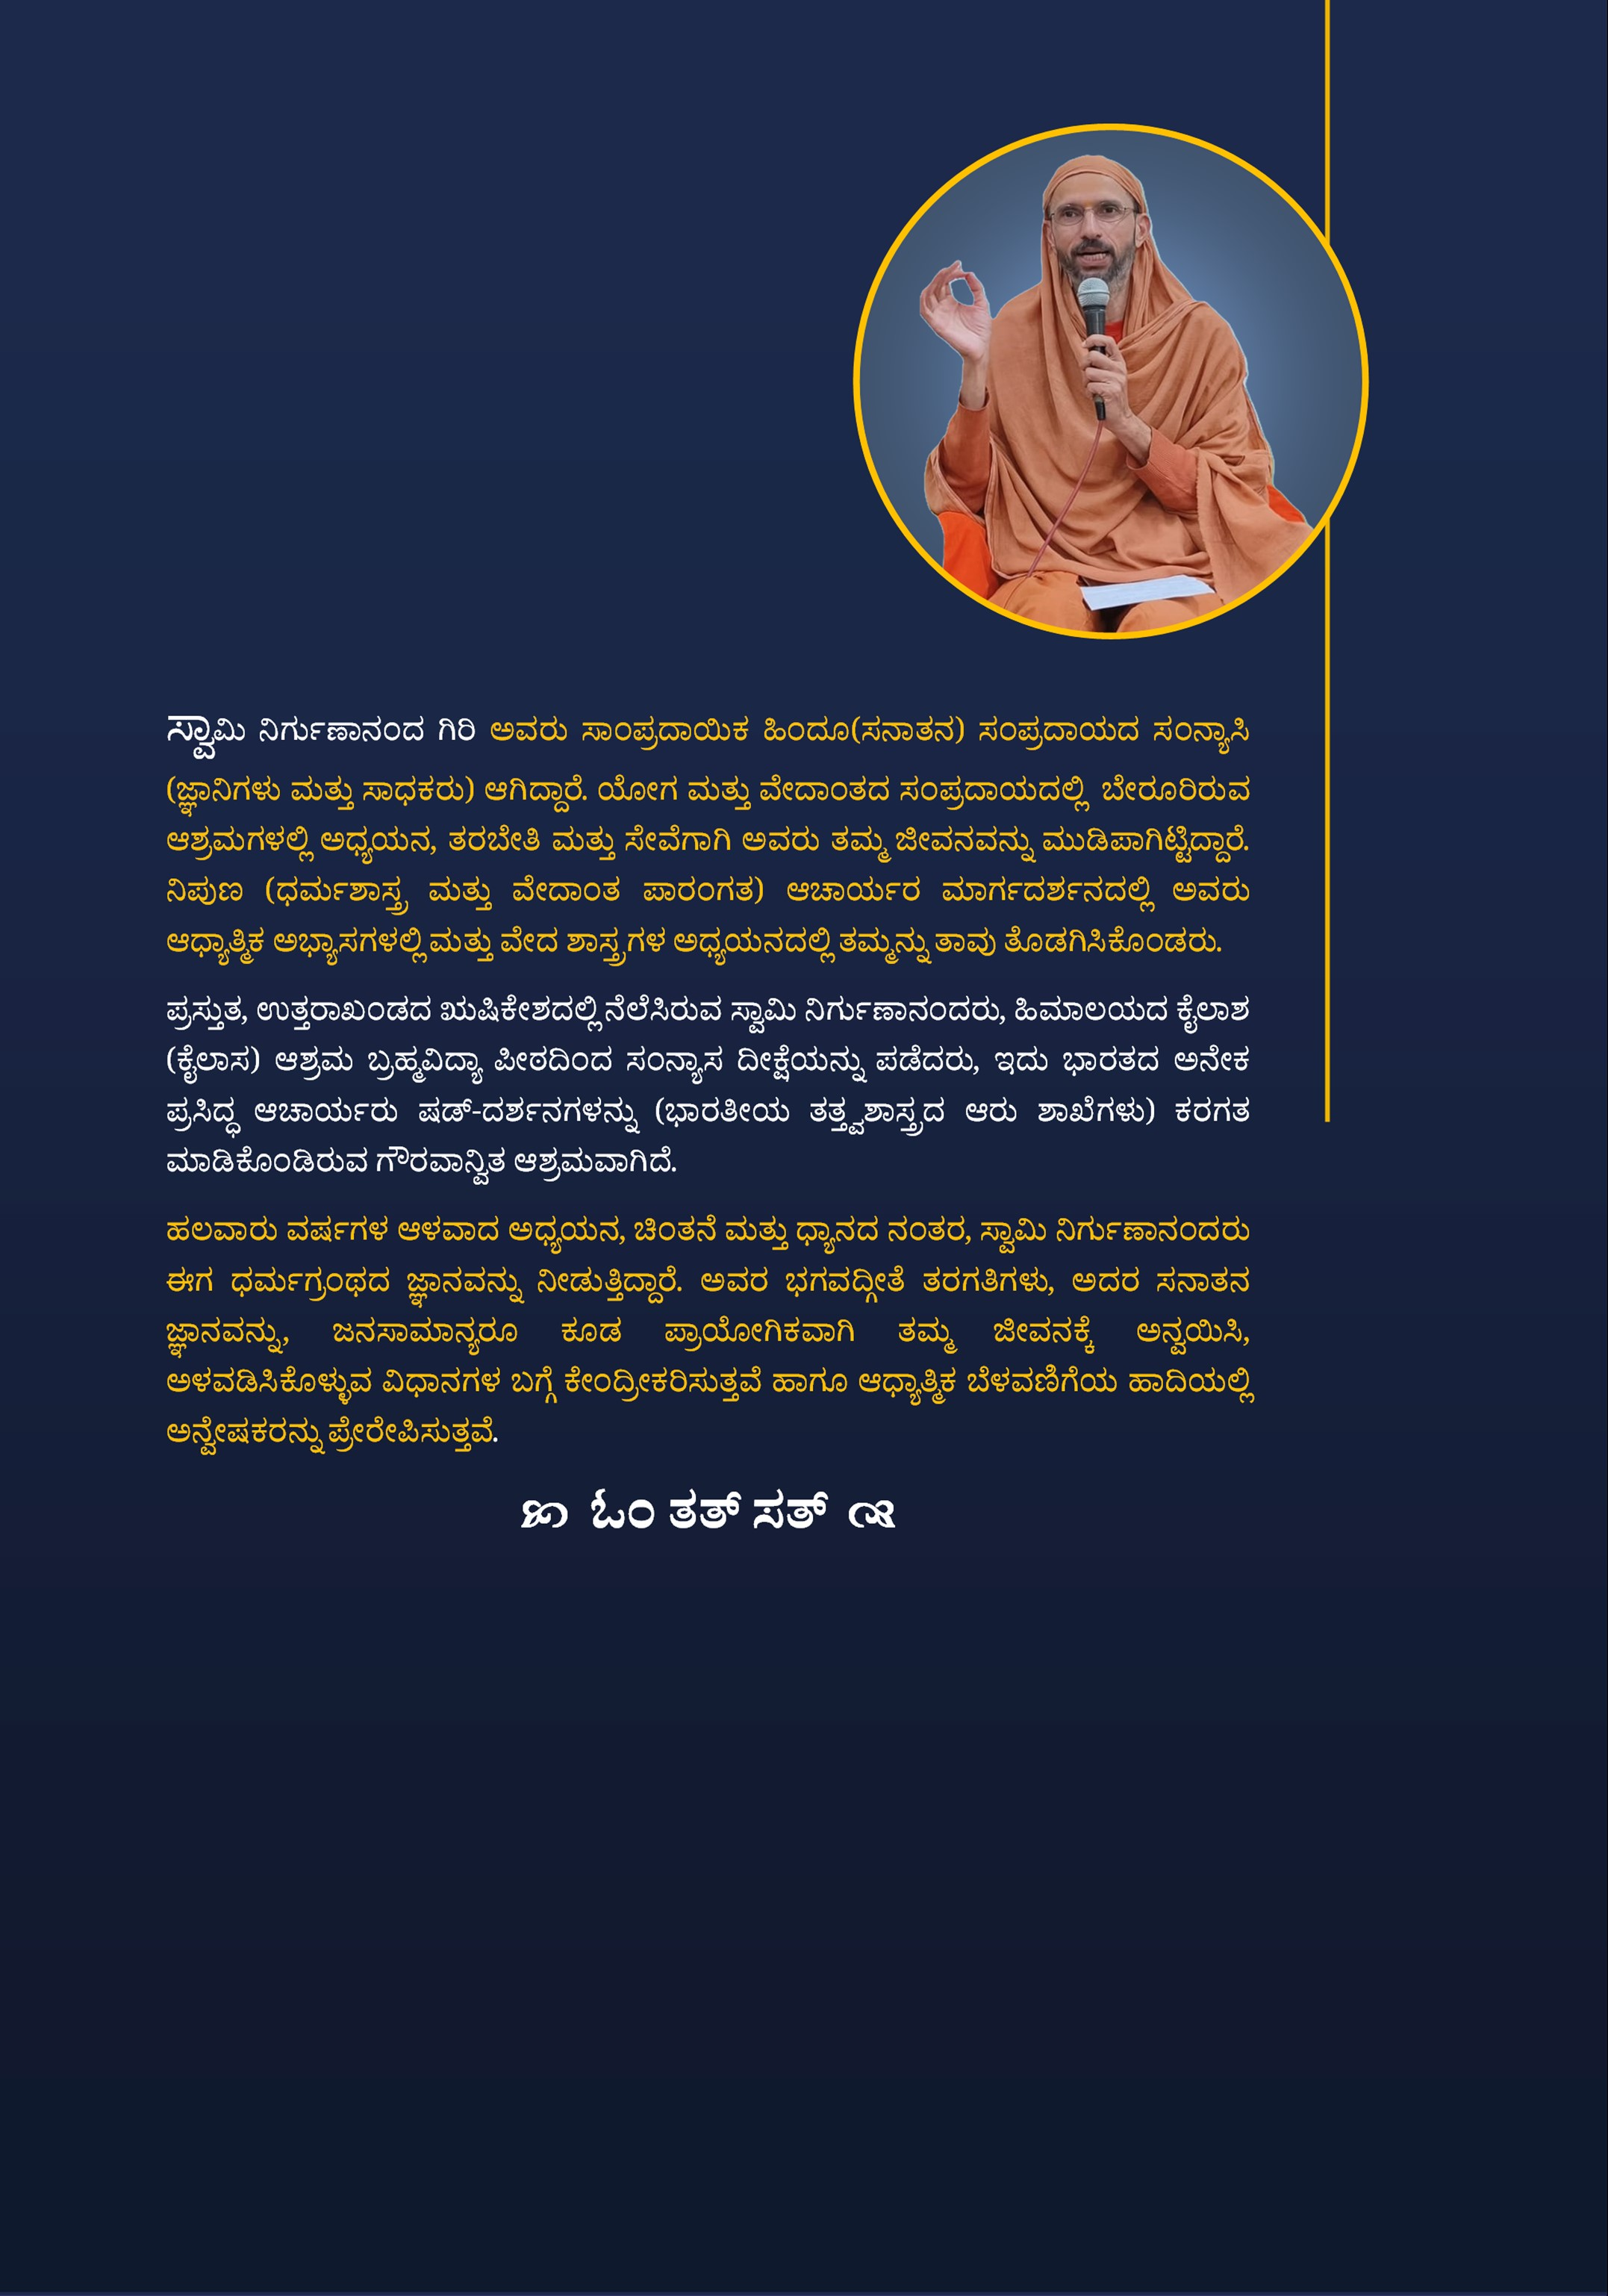
\includegraphics[width=\paperwidth,height=\paperheight]{./images/page02.jpg}%
    }%
	}
   \else% do nothing
   \AddToShipoutPictureBG*{%
    \AtPageLowerLeft{%
        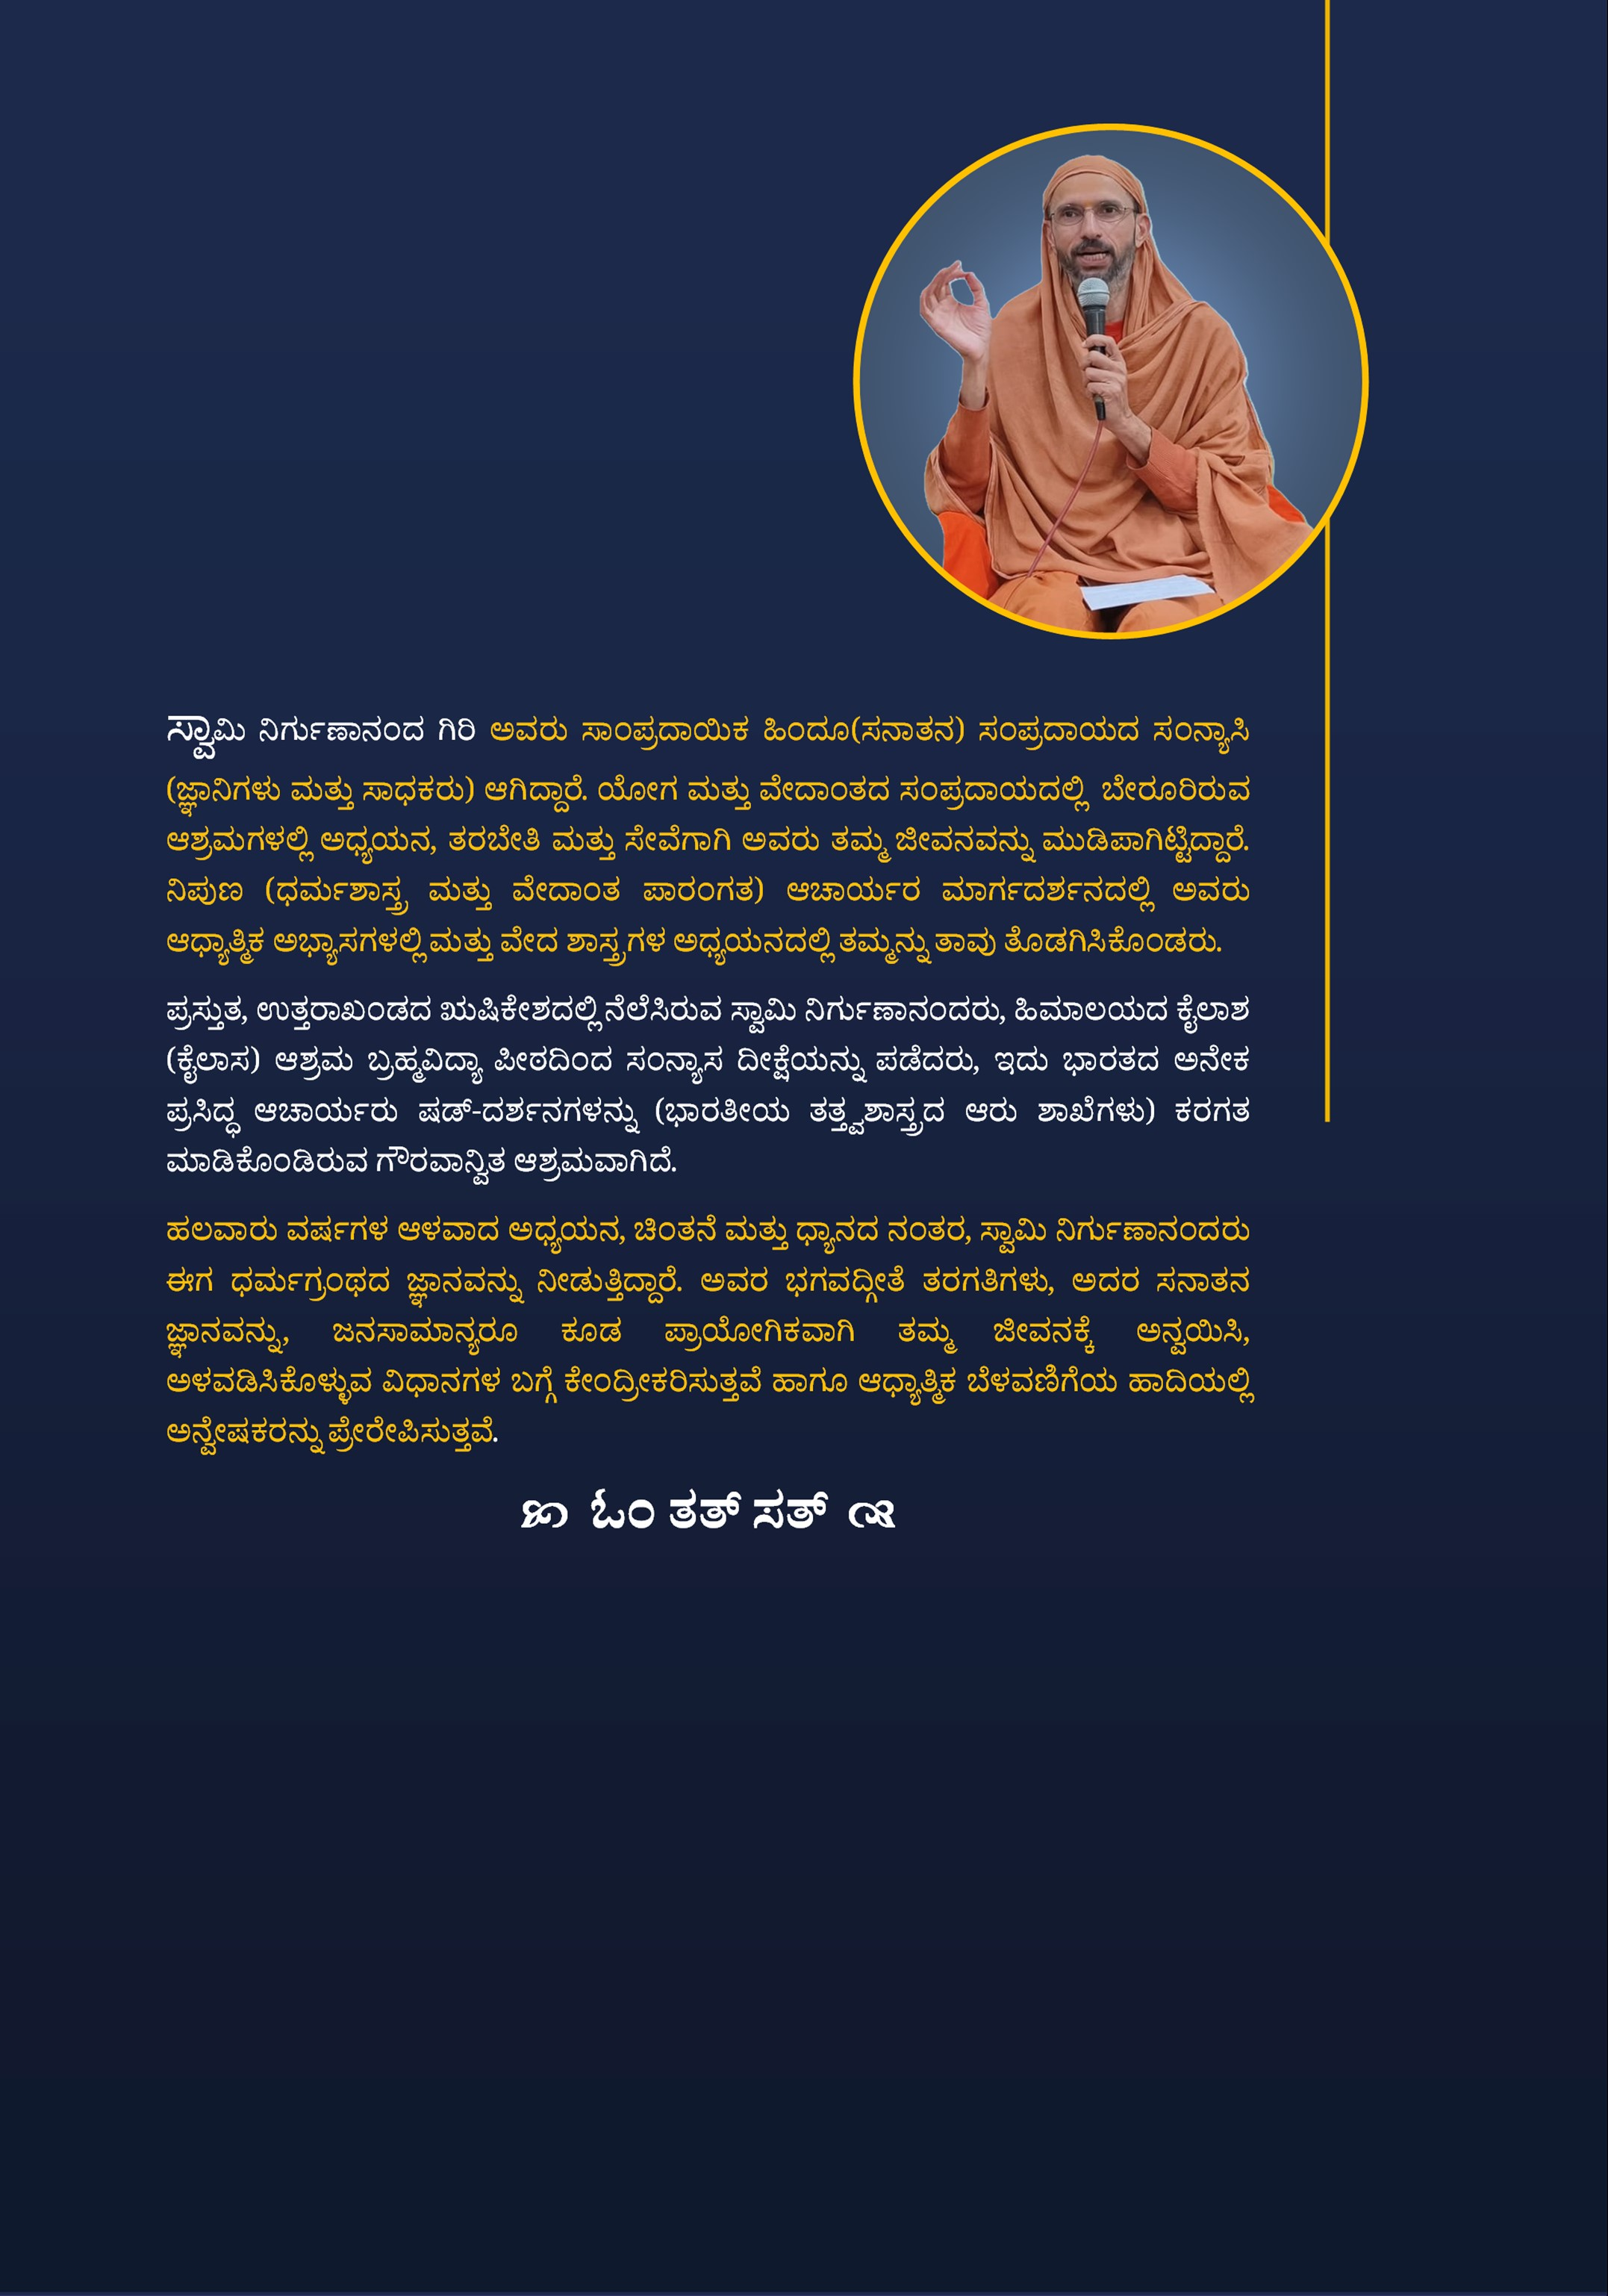
\includegraphics[width=\paperwidth,height=\paperheight]{./images/page02.jpg}%
    }%
	}
\fi
\begin{titlepage}
	%\pagecolor{pastelblue}
	\AddToShipoutPictureBG*{%
    \AtPageLowerLeft{%
        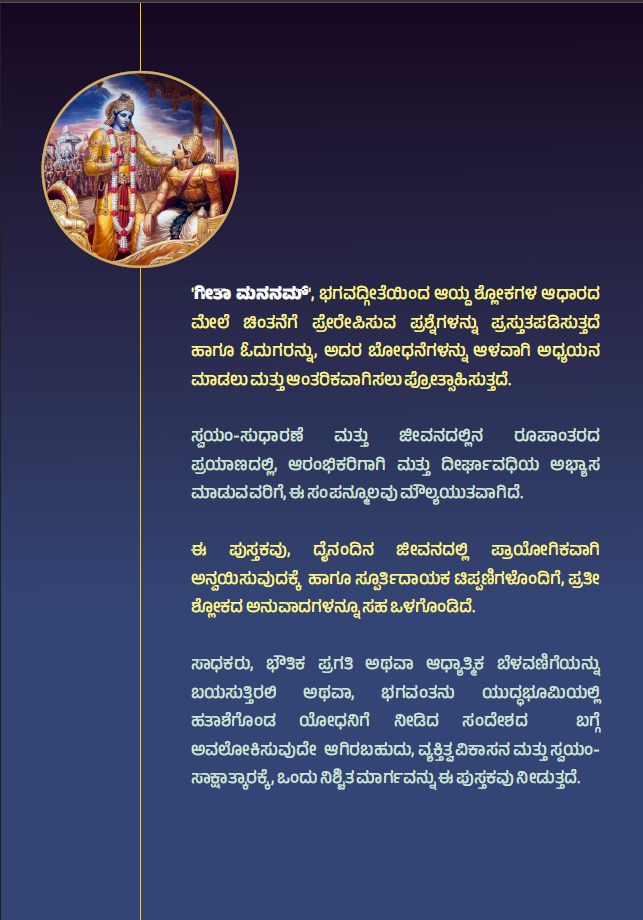
\includegraphics[width=\paperwidth,height=\paperheight]{./images/backcover.png}%
    }%
}
    \begin{center}
        \vspace*{0.5cm}
            
        {\Huge
        %\textbf{\color{white}\fontsize{50}{60}\selectfont ಗೀತಾ ಮನನಂ}
		}
        %\textbf{\\ \small \color{white}ದೈನಂದಿನ ಸ್ಪೂರ್ತಿ ಹಾಗೂ ಆತ್ಮಾವಲೋಕನಕ್ಕಾಗಿ}    
        \vspace{1.0cm}
            
        
		
            
        \vfill
            
        
            
        \vspace{0.1cm}
        {\color{white}    
		%\textbf{{\Large \mananamfont ಸ್ವಾಮಿ ನಿರ್ಗುಣಾನಂದ ಗಿರಿ}}\\
		%{\normalsize Swami Nirgunananda Giri\\Rishikesh, India}
        }
    \end{center}
\end{titlepage}
\nopagecolor% Use this to restore the color pages to white
\end{document}
